\documentclass{report}
\title{`Mathematics for Machine Learning'---Notes}
\date{Started 8 July 2024}
\author{Malcolm}
\usepackage{amsmath} %import math
\usepackage{mathtools} %more math
\usepackage{amssymb} %for QED symbol
\usepackage{amsthm} %
\usepackage{bm} %bolding without changing font
\usepackage{graphicx} %import imaging
\graphicspath{{./images/}} %set imaging path
\begin{document}
\maketitle
\tableofcontents

\appendix
\chapter{Linear Algebra}
\section{Fundamentals}
\subsection{Groups}
Given a set $\mathcal{G}$ and an operation $\otimes:\mathcal{G\times G\rightarrow G}$ defined on
$\mathcal{G}$, then $G:=(\mathcal{G},\otimes)$ is called a \textit{group} if the following hold:
\begin{enumerate}
\item \textit{Closure} of $\mathcal{G}$ under $\otimes:
\forall x,y\in\mathcal{G}:x\otimes y
\in\mathcal{G}$
\item\textit{Associativity}: $\forall x,y,z\in\mathcal{G}:(x\otimes y)\otimes z=x\otimes(y\otimes z)$
\item\textit{Neutral element}: $\exists e\in\mathcal{G}\,\forall x\in\mathcal{G}:
x\otimes e=x$ and $e\otimes x=x$
\item\textit{Inverse element}: $\forall x\in\mathcal{G}\,\exists y\in\mathcal{G}:x\otimes y=e$
and $y\otimes x=e$, where $e$ is the neutral element.
\end{enumerate}
The neutral element in the depends on $\otimes$.\\
\vspace{1mm}\\
\textbf{Abelian groups}\\
If \textit{Commutativity}: $\forall x,y\in\mathcal{G}:x\otimes y=y\otimes x$ holds, then 
$G=(\mathcal{G},\otimes)$ is an \textit{Abelian group}\\
\vspace{1mm}\\
\textbf{Examples}
\begin{itemize}
\item$(\mathbb{Z},+)$ is an Abelian group
\item$(\mathbb{N}_0,+)$ is not a group; although $(\mathbb{N}_0,+)$ possesses a neutral
element (0), the inverse elements are missing.
\item$(\mathbb{Z},\cdot)$ is not a group; although $(\mathbb{Z},\cdot)$ contains the neutral element (1),
the inverse elements for any $z\in\mathbb{Z},\,z\neq\pm1$,
are missing
\item$(\mathbb{R}^n,+),(\mathbb{Z}^n,+),n\in\mathbb{N}$ are Abelian if + is defined componentwise, i.e.,
\begin{equation*}
(x_1,\ldots,x_n)+(y_1,\ldots,y_n)=(x_1+y_1,\ldots,x_n+y_n)
\end{equation*}
Where $(-x_1,\ldots,-x_n)$ is the inverse element and $e=(0,\ldots,0)$ is the neutral element
\end{itemize}
\newpage

\subsection{Vector Spaces} %140724
A real-valued vector space $V=(\mathcal{V},+,\cdot)$ is a set $\mathcal{V}$ with two operations
\begin{align*}
+:\mathcal{V\times V\to V}\\
\cdot:\mathbb{R}\times\mathcal{V}\to\mathcal{V}
\end{align*}
(the first operation + is an inner operation (mappings that only operate on elements in $\mathcal{G}$); the 
other operation is the multiplication of a vector $x\in\mathcal{G}$ by a scalar $\lambda\in\mathbb{R}$. 
We can think of the inner operation as a form of addition,
and the outer operation as a form of scaling.)\\
\vspace{1mm}\\
where
\begin{enumerate}
\item$\mathcal{(V,+)}$ is an Abelian group
\item Distributivity:
\begin{itemize}
\item$\forall\lambda\in\mathbb{R},x,y\in\mathcal{V}:
\lambda\cdot(x+y)=\lambda\cdot x+\lambda\cdot y$
\item$\forall\lambda,\psi\in\mathbb{R},x\in\mathcal{V}:
(\lambda+\psi)\cdot x=\lambda\cdot x+\psi\cdot x$
\end{itemize}
\item Associativity (outer operation):
$\forall\lambda,\psi\in\mathbb{R},x\in\mathcal{V}
:\lambda\cdot(\psi\cdot x)=(\lambda\cdot\psi)\cdot x$
\item Neutral element with respect to the outer operation:
$\forall x\in\mathcal{V}:1\cdot x=x$
\end{enumerate}
(the neutral element of $(\mathcal{V.+})$ is the zero vector $\mathbf{0}=[0,\ldots,0]^T$) Note that
the ''vector multiplication'' $ab,a,b\in\mathbb{R}^n$, is not defined only the following
multiplications for vectors are defined: $ab^T\in\mathbb{R}^{n\times n}$ 
(outer product), $a^Tb\in\mathbb{R}$
(inner/scalar/dot product).\\
\vspace{1mm}\\
\textbf{Example:}\\
$\mathcal{V}=\mathbb{R}^{m\times n},m,n\in\mathbb{N}$ is a
vector space with
\begin{itemize}
\item Addition: $A+B=\begin{bmatrix}
a_{11}+b_{11}&\cdots&a_{1n}+b_{1n}\\
\vdots&&\vdots\\
a_{m1}+b_{m1}&\cdots&a_{mn}+b_{mn}
\end{bmatrix}$ defined elementwise for all $A,B\in\mathcal{V}$.
\item Multiplication by scalars: 
$\lambda A=\begin{bmatrix}
\lambda a_{11}&\cdots&\lambda a_{1n}\\
\vdots&&\vdots\\
\lambda a_{m1}&\cdots&\lambda a_{mn}
\end{bmatrix}$ 
\end{itemize}
\newpage

\subsection{Vector Subspaces}
Let $V=(\mathcal{V,+,\cdot})$ be a vector space and $\mathcal{U\subseteq V,\,U\neq\emptyset}$. 
Then $U=(\mathcal{U},+,\cdot)$ is called a \textit{vector subspace/linear subspace} of $V$ if $U$ 
is a vector space with the vector space operations + and $\cdot$ restricted to 
$\mathcal{U\times U}$ and $\mathbb{R}\times\mathcal{U}$. We write $U\subseteq V$ to denote a subspace $U$ of $V$.\\
\vspace{1mm}\\
\textbf{Properties}\\
If $\mathcal{U\subseteq V}$ is a vector space, then $U$ naturally inherits many properties from $V$, since
they hold for all $x\in V$, and thus 
$x\in\mathcal{U\in V}$.\\
\vspace{1mm}\\
These include the \textit{Abelian group properties, distributivity, associativity, and the neutral element}.
To determine whether $(\mathcal{U},+,\cdot)$ is a valid subspace of $V$ need to show
\begin{enumerate}
\item$\mathcal{U}\neq\emptyset$, in particular: $\mathbf{0}\in\mathcal{U}$
\item Closure of $U$:
\begin{enumerate}
\item With respect to the outer operation: 
$\forall\lambda\in\mathbb{R}\,\forall x\in\mathcal{U}:\lambda x\in\mathcal{U}$
\item With respect to the inner operation:
$\forall x,y\in\mathcal{U}:x+y\in\mathcal{U}$
\end{enumerate}
\end{enumerate}
\newpage

\subsection{Are linear combinations of linearly independent\\vectors also linearly independent?} %150724
\label{fundamentals:ALCOLIVALI}
Consider a vector space $V$ with $k$ linearly independent vectors $b_1\ldots b_k$; 
consider $m$ linear combinations of these vectors:
\begin{align*}
x_1&=\sum^k_{i=1}\lambda_{i1}b_i\\
&\vdots\\
x_m&=\sum^k_{i=1}\lambda_{im}b_i
\end{align*}
Defining $B=[b_1\ldots b_k]$ as a matrix with columns being the linearly independent vectors $b_1\ldots b_k$,
we can write
\begin{equation*}
x_j=B\lambda_j,\quad\lambda_j=\left[\begin{array}{c}
\lambda_{1j}\\\vdots\\\lambda_{kj}\end{array}\right],
\quad j=1,\ldots,m
\end{equation*}
We want to test whether $x_1,\ldots,x_m$ are linearly independent. Using the general 
approach (whether $\sum^m_{j=1}\psi_jx_j=0$ has nontrivial solutions):
\begin{equation*}
\sum^{m}_{j=1}\psi_jx_j
=\sum^{m}_{j=1}\psi_jB\lambda_j
=B\sum^{m}_{j=1}\psi_j\lambda_j
\end{equation*}
This means that $\{x_1,\ldots,x_m\}$ are linearly independent if and only if
the column vectors $\{\lambda_1,\ldots,\lambda_m\}$ are linearly independent.
\newpage

\subsection{Generating Set, Basis, Span} %150724
\textbf{Generating set, Span}\\
Consider a vector space $V=(\mathcal{V},+,\cdot)$ and a set of vectors 
$\mathcal{A}=\{x_1,\ldots,x_k\}\subseteq\mathcal{V}$. If every vector $v\in\mathcal{V}$ can be 
expressed as a linear combination of $x_1,\ldots,x_k$, $\mathcal{A}$ is called a \textit{generating
set} of $V$.\\
\vspace{1mm}\\
The set of all linear combinations of vectors in $\mathcal{A}$ is called the \textit{span} of $\mathcal{A}$. 
Where $\mathcal{A}$ spans the vector space $V$, we write
$V=\text{span}[\mathcal{A}]$ or 
$V=\text{span}[x_1,\ldots,x_k]$.\\
\vspace{1mm}\\
Intuitively, every vector in a vector (sub)space can be represented as a
linear combination of the vectors in the generating set that spans that vector (sub)space.\\
\vspace{1mm}\\
\textbf{Basis}\\
Consider a vector space $V=(\mathcal{V},+,\cdot)$ and
$\mathcal{A}\subseteq\mathcal{V}$. A generating set $\mathcal{A}$ of $V$ is called 
\textit{minimal} if there exists no smaller set 
$\tilde{\mathcal{A}}\subseteq\mathcal{A}\subseteq\mathcal{V}$
that spans $V$. Every linearly independent generating set of $V$ is minimal and is called the 
\textit{basis} of $V$.\\
\vspace{1mm}\\
For intuition, let $V=(\mathcal{V},+,\cdot)$ be a vector space and 
$\mathcal{B}\subseteq\mathcal{V},\mathcal{B}\neq\emptyset$. Then the following statements are equivalent:
\begin{itemize}
\item$\mathcal{B}$ is a basis of $V$
\item$\mathcal{B}$ is a minimal generating set
\item$\mathcal{B}$ is a maximal linearly independent set of vectors in $V$ 
(adding any other vector in $V$ to this set would make it linearly dependent).
\item Every vector $x\in V$ is a linear combination of vectors from $B$, and every linear combination is unique;
with 
\begin{equation*}
x=\sum^k_{i=1}\lambda b_i=\sum^k_{i=1}\psi b_i
\end{equation*}
and $\lambda_i,\psi_i\in\mathbb{R}$ it follows that 
$\lambda_i=\psi_i,\,i=1\ldots k$.
\end{itemize}
\newpage

\subsection{Dimensionality (finding a basis)} %160724
\textbf{Dimensionality}\\
Considering finite-dimensional vector spaces $V$, the \textit{dimension} of $V$ is the number
of basis vectors of $V$, written as $\dim{V}$. If $U\subseteq V$ is a subspace of $V$, then
$\dim(U)\leq\dim(V)$ and $\dim(U)=\dim(V)$ if and only if
$U=V$. Finding the dimension of a vector space is therefore the same as finding a basis.\\
\vspace{1mm}\\
\textbf{Determining a Basis}\\
The basis of a subspace $U=\text{span}[x_1,\ldots,x_m]\subseteq\mathbb{R}^n$ can be found using the 
protocol:
\begin{enumerate}
\item Write the spanning vectors as columns of a matrix $A$
\item Determine the row-echelon form of $A$
\item The spanning vectors associated with the pivot columns are a basis of $U$
\end{enumerate}
Consider an example: for a vector subspace $U\subseteq\mathbb{R}^5$, spanned by the vectors
\begin{equation*}
x_1=\begin{bmatrix*}[c]
1\\2\\-1\\-1\\-1
\end{bmatrix*},\quad
x_2=\begin{bmatrix*}[c]
2\\-1\\1\\2\\-2
\end{bmatrix*},\quad
x_3=\begin{bmatrix*}[c]
3\\-4\\3\\5\\-3
\end{bmatrix*},\quad
x_4=\begin{bmatrix*}[c]
-1\\8\\-5\\-6\\1
\end{bmatrix*},\in\mathbb{R}^5
\end{equation*}
in order to determine which vectors $x_1\ldots x_4$ are a basis for $U$, we need to check
whether they are linearly independent; we need to solve
\begin{equation*}
\sum^4_{i=1}\lambda_ix_i=\mathbf{0}
\end{equation*}
Notice this can be viewed as solving the system represented by the augmented matrix
\begin{equation*}
\left[\begin{array}{cccc|c}
\vdots&\vdots&\vdots&\vdots&\vdots\\
x_1&x_2&x_3&x_4&\mathbf{0}\\
\vdots&\vdots&\vdots&\vdots&\vdots
\end{array}\right]
\end{equation*}
(thus the 'augmented' part of the matrix can simply be ignored since gaussian elimination won't alter it)\\
(next page)
\newpage
\noindent Using gaussian elimination to obtain the row-echelon form:
\begin{equation*}
\begin{bmatrix*}[c]
1&2&3&-1\\
2&-1&-4&8\\
-1&1&3&-5\\
-1&2&5&-6\\
-1&-2&-3&1
\end{bmatrix*}\rightsquigarrow\cdots\rightsquigarrow
\begin{bmatrix*}[c]
1&2&3&-1\\
0&1&2&-2\\
0&0&0&1\\
0&0&0&0\\
0&0&0&0
\end{bmatrix*}
\end{equation*}
The non-pivot column corresponds to the vector in the generating set that can be expressed
as a linear combination of the other vectors in that generating set. 
The pivot columns indicate which set of vectors are linearly independent.\\
\vspace{1mm}\\
From the pivot columns of the row-echelon form we see that $x_1,x_2,x_4$ are linearly independent. 
Therefore, $\{x_1,x_2,x_4\}$ is a basis of $U$.
\newpage

\subsection{Rank} %160724
The number of linearly independent columns of matrix $A\in\mathbb{R}^{m\times n}$ equals the number
of linearly independent rows and is called the \textit{rank} of $A$, denoted by $\text{rk}(A)$.\\
\vspace{1mm}\\
\textbf{Properties}
\begin{itemize}
\item rk$(A)$=rk$(A^T)$; the column rank equals the row rank.
\item The columns of $A\in\mathbb{R}^{m\times n}$ span a subspace $U\subseteq\mathbb{R}^m$ 
(the number of rows determine the dimension the vector exists in) 
with $\dim(U)=\text{rk}(A)$ this subspace is the \textit{image/range}, with basis found 
through Gaussian elimination of $A$ to identify the pivot columns.
\item The rows of $A\in\mathbb{R}^{m\times n}$ span a subspace $W\subseteq\mathbb{R}^n$
with $\dim(W)=\text{rk}(A)$. A basis for $W$ can be found by Gaussian elimination of $A^T$.
\item For all $A\in\mathbb{R}^{n\times n}$ it holds that $A$ is regular/invertible if and only if
rk$(A)=n$ (full rank).
\item For all $A\in\mathbb{R}^{m\times n}$ and all $b\in\mathbb{R}^m$
it holds that the linear equation system $Ax=b$ can be solved if and only if rk$(A)$=rk$(A|b)$, 
where $A|b$ denotes the augmented system (otherwise there will be a contradiction).
\item For $A\in\mathbb{R}^{m\times n}$ the subspace of solutions for $Ax=\mathbf{0}$ possesses dimension
$n-\text{rk}(A)$. This subspace is the \textit{kernel/nullspace}.
\item A matrix $A\in\mathbb{R}^{m\times n}$ has \textit{full rank} if its rank is equal to the largest
possible rank for a matrix of the same dimensions; meaning rk$(A)=\min(m,n)$. A matrix is \textit{rank deficient} if it is not full rank.
\end{itemize}
\newpage

\subsection{Linear Mappings} %160724
\label{fundamentals:linear mappings}
Consider two real vector spaces $V,W$. A mapping $\Phi:V\rightarrow W$ preserves
the structure of the vector space if
\begin{align*}
\Phi(x+y)&=\Phi(x)+\Phi(y)\\
\Phi(\lambda x)&=\lambda\Phi(x)
\end{align*}
for all $x,y\in V$ and $\lambda\in\mathbb{R}$.\\
\vspace{1mm}\\
For vector spaces $V,W$, a mapping $\Phi:V\rightarrow W$ is called a 
\textit{linear mapping/vector space homomorphism/linear transformation} if
\begin{equation*}
\forall x,y\in V\,\forall\lambda,\psi\in\mathbb{R}:\Phi(\lambda x+\psi y)
=\lambda\Phi(x)+\psi\Phi(y)
\end{equation*}
(\textit{Homo-} meaning 'same' and \textit{-morph} meaning 'form' or 'shape) 
Linear mappings can be represented by matrices.\\
\vspace{1mm}\\
Consider a mapping $\Phi:\mathcal{V\rightarrow W}$, where $\mathcal{V,W}$ can be arbitrary sets.
Then $\Phi$ is called
\begin{itemize}
\item\textit{Injective} if $\forall x,y\in\mathcal{V}:
\Phi(x)=\Phi(y)\implies x=y$.
\item\textit{Surjective} if $\Phi(\mathcal{V)=W}$.
\item\textit{Bijective} if it is injective and surjective.
\end{itemize}
Intuitively, if $\Phi$ is surjective, then every element in $\mathcal{W}$ can be 
'reached' from $\mathcal{V}$. A bijective $\Phi$ can be 'undone', 
meaning there exists a mapping $\Psi:\mathcal{W\to V}$ so that $\Psi\circ\Phi(x)=x$. 
This mapping $\Psi$ can then be called the inverse of $\Phi$ and be denoted by $\Phi^{-1}$.\\
\vspace{1mm}\\
Now we define special cases of linear mappings between vector spaces $V$ and $W$:
\begin{itemize}
\item\textit{Isomorphism}: $\Phi:V\to W$ linear and bijective
\item\textit{Endomorphism}: $\Phi:V\to V$ linear
\item\textit{Automorphism}: $\Phi:V\to V$ linear and bijective
\item We define $\text{id}_V:V\to V,x\mapsto x$ as the \textit{identiy mapping/identity automorphism}.
\end{itemize}
(next page)
\newpage
\noindent\textbf{Example}: Homomorphism\\
The mapping $\Phi:\mathbb{R}^2\rightarrow\mathbb{C},\Phi(x)=x_1+ix_2$, is a homomorphism since
\begin{align*}
\Phi\left(\begin{bmatrix}x_1\\x_2\end{bmatrix}+
\begin{bmatrix}y_1\\y_2\end{bmatrix}\right)
&=(x_1+y_1)+i(x_2+y_2)=x_1+ix_2+y_1+iy_2\\
&=\Phi\left(\begin{bmatrix}x_1\\x_2\end{bmatrix}\right)
+\Phi\left(\begin{bmatrix}y_1\\y_2\end{bmatrix}\right)
\end{align*}
and
\begin{equation*}
\Phi\left(\lambda\begin{bmatrix}x_1\\x_2\end{bmatrix}\right)=\lambda x_1+\lambda ix_2=\lambda(x_1+ix_2)
=\lambda\Phi\left(\begin{bmatrix}x_1\\x_2\end{bmatrix}\right)
\end{equation*}
Notice that this justifies why complex numbers can be represented as tuples in $\mathbb{R}^2$.\\
\vspace{1mm}\\
\textbf{Theorem}: \textit{Finite-dimensional vector spaces $V$ and $W$ are isomorphic
if and only if $\dim(V)=\dim(W)$.}\\
\vspace{1mm}\\
This theorem states that there exists a linear, bijective mapping between two vector
spaces of the same dimension. Intuitively this means that vector spaces
of the same dimension are kind of the same thing, since they can be 
transformed into each other without incurring any loss.
\newpage

\subsection{Matrix Representation of Linear Mappings}%170724
\textbf{Ordered Basis}\\
Any $n$-dimensional vector space is isomorphic to $\mathbb{R}^n$\ (\ref{fundamentals:linear mappings}).
Consider a basis $\bm{\{b_1\ldots b_n\}}$ of an $n$-dimensional vector space $V$; in the following 
the order of the basis vectors will be important, so we write
\begin{equation*}
B=\bm{(b_1\ldots b_n)}
\end{equation*}
and call this $n$-tuple an \textit{ordered basis} of $V$.\\
(Just a note on notation: $B=\bm{(b_1\ldots b_n)}$ is an ordered basis, 
$B=\bm{\{b_1\ldots b_n\}}$ is an (unordered) basis,
and $B=\bm{[b_1\ldots b_n]}$ is a matrix whose columns are the vectors $\bm{b_1\ldots b_n}$.)\\
\vspace{1mm}\\
\textbf{Coordinates}\\
Consider a vector space $V$ and an ordered basis $B=\bm{(b_1\ldots b_n)}$ of $V$. 
For any $x\in V$ we have a unique representation (through a linear combination)
\begin{equation*}
x=\alpha_1\bm{b_1}+\ldots+\alpha_n\bm{b_n}
\end{equation*}
of $x$ with respect to $B$. Then $\alpha_1\ldots\alpha_n$ are the \textit{coordinates}
of $x$ with respect to $B$, and the vector 
\begin{equation*}
\bm{\alpha}=\begin{bmatrix}\alpha_1\\\vdots\\\alpha_n
\end{bmatrix}\in\mathbb{R}^n
\end{equation*}
is the \textit{coordinate vector/coordinate representation} of $x$
with respect to the ordered basis $B$.\\
\vspace{1mm}\\
Intuitively, a basis effectively defines a coordinate system. One is usually familiar with
the canonical basis vectors $\bm{e_1,e_2}$; notice that a vector in this coordinate system
$x\in\mathbb{R}^2$ can also be seen as a representation describing how to linearly combine
$\bm{e_1,e_2}$ to obtain $x$.\\
\vspace{1mm}\\
However, any basis of $\mathbb{R}^2$ defines a valid coordinate system; the same vector $x$ from before 
may therefore have a different representation in the 
$\bm{(b_1,b_2)}$ basis.\\
(next page)
\newpage
\noindent\textbf{Example}\\
Consider how the same vector can be represented differently in two different basis representations.
\begin{figure}[h]
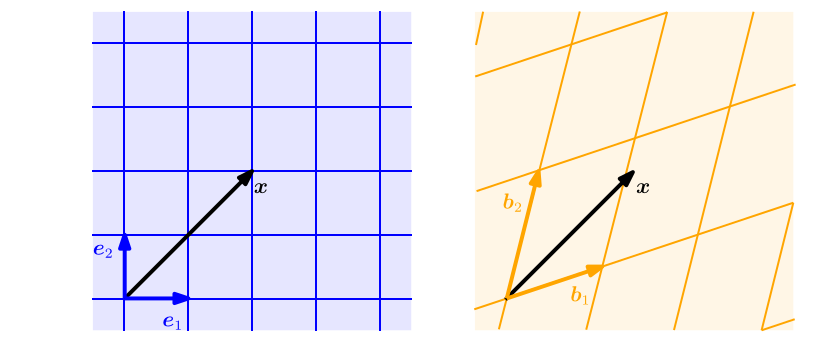
\includegraphics[width=10cm]{1}\\
\centering
\end{figure}\\
In the above figure, the coordinates of $x$ with respect to the standard basis is $[2,2]^T$,
but with respect to the basis ($\bm{b_1,b_2}$) the same vector $x$ is represented as $[1.09,0.72]^T$, 
where $x=1.09\bm{b_1}+0.72\bm{b_2}$ instead of $x=2\bm{e_1}+2\bm{e_2}$.\\
\vspace{1mm}\\
\textbf{Another Example}\\
The geometric vector $x\in\mathbb{R}^2$ with coordinates
$[2,3]^T$ with respect to the standard basis $\bm{e_1,e_2}$ of $\mathbb{R}^2$ can be written as 
$x=2\bm{e_1}+3\bm{e_2}$. However we don't necessarily have to use the standard basis to represent it;
if we use the basis $\bm{b_1}=[1,-1]^T,\bm{b_2}=[1,1]^T$ we obtain the coordinates $\frac{1}{2}[-1,5]^T$
to represent the same vector with respect to $(\bm{b_1,b_2})$; $x=-1/2\cdot\bm{b_1}+5/2\cdot\bm{b_2}$.\\
\vspace{1mm}\\
\textit{Remark.} For an $n$-dimensional space $V$ and an ordered basis $B$ of $V$, the mapping
$\Phi:\mathbb{R}^n\rightarrow V,\Phi(e_i)=b_i,i=1\ldots n$, is linear 
(and because of (\ref{fundamentals:linear mappings}) an isomorphism), where ($\bm{e_1\ldots e_n}$) 
is the standard basis of $\mathbb{R}^n$.\\
\vspace{1mm}\\
Note that a \textit{mapping} and a \textit{change of basis} (like the examples above) are different.\\
(next page)
\newpage
\noindent\textbf{Transformation Matrix}\\
Consider vector spaces $V,W$ with corresponding (ordered) bases $B=(\bm{b_1\ldots b_n})$
and $C=(\bm{c_1\ldots c_m})$. Now consider a linear mapping 
$\Phi:V\rightarrow W$. For $j\in\{1,\ldots,n\}$,
\begin{equation*}
\Phi(\bm{b_j})=\alpha_{1j}\bm{c_1}+\ldots+
\alpha_{mj}\bm{c_m}=\sum^{m}_{i=1}\alpha_{ij}\bm{c_i}
\end{equation*}
is the unique representation of $\Phi(\bm{b_j})$ with respect to the ordered basis $C$. 
We call this $m\times n$-matrix $A_\Phi$, whose elements are given by
\begin{equation*}
A_\Phi(i,j)=\alpha_{ij}
\end{equation*}
the \textit{transformation matrix} of $\Phi$ (with respect to the ordered bases $B$ of $V$ and $C$ of $W$).\\
\vspace{1mm}\\
The coordinates of $\Phi(\bm{b_j})$ with respect to the ordered basis $C$ of $W$ are the $j$-th column of
$A_\Phi$. If $\hat{\bm{x}}$ is the coordinate vector of $x\in V$ with respect to $B$ and 
$\hat{\bm{y}}$ the coordinate vector of $y=\Phi(x)\in W$ with respect to $C$, then
\begin{equation*}
\hat{\bm{y}}=\bm{A_\Phi\hat{x}}
\end{equation*}
the transformation matrix can be used to map coordinates with respect to an ordered basis in $V$
to coordinates with respect to an ordered basis in $W$.\\
\vspace{1mm}\\
\textbf{Intuition}\\
Consider coordinate vector $[a,b,c,\ldots]^T$ in $V$ with basis $B$ (meaning the vector in $V$ is 
expressed as $a\bm{b_1}+b\bm{b_2}+\ldots$). Now consider applying a linear mapping $\Phi:V\rightarrow W$,
where $W$ is has basis $C$, to $V$:
\begin{equation*}
\Phi(a\bm{b_1}+b\bm{b_2}+\ldots)=a\Phi(\bm{b_1})+b\Phi(\bm{b_2})+\ldots
\end{equation*}
we express each basis vector of $B$ in terms of $C$; for $j\in\{1,\ldots,n\}$,
\begin{equation*}
\Phi(\bm{b_j})=\alpha_{1j}\bm{c_1}+\ldots+
\alpha_{mj}\bm{c_m}
\end{equation*}
so
\begin{align*}
&a\Phi(\bm{b_1})+b\Phi(\bm{b_2})+\ldots\\
=&a(\alpha_{11}\bm{c_1}+\ldots+\alpha_{m1}\bm{c_m})
+b(\alpha_{12}\bm{c_1}+\ldots+\alpha_{m2}\bm{c_m})+\ldots\\
=&\underbrace{(a\alpha_{11}+b\alpha{12}+\ldots)}_{\text{first coordinate}}\bm{c_1}+
(a\alpha_{m1}+b\alpha{m2})\bm{c_m}+\ldots
\end{align*}
which leads to our compact representation $\hat{\bm{y}}=\bm{A_\Phi\hat{x}}$. 
\newpage

\subsection{Basis Change} %170724
\label{fundamentals:basis change}
\textbf{Intuition}\\
Consider two ordered bases of $V$:
\begin{equation*}
B=(\bm{b_1,\ldots,b_n}),\quad\tilde{B}=(\bm{\tilde{b_1}},\ldots,\bm{\tilde{b_n}})
\end{equation*}
and two ordered bases of $W$:
\begin{equation*}
C=(\bm{c_1,\ldots,c_m}),\quad\tilde{C}=(\bm{\tilde{c_1}},\ldots,\bm{\tilde{c_m}})
\end{equation*}
We define $\bm{A_\Phi}\in\mathbb{R}^{m\times n}$ be the transformation matrix of the linear mapping 
$\Phi:V\rightarrow W$ with respect to bases $B$ and $C$, and 
$\tilde{\bm{A_\Phi}}\in\mathbb{R}^{m\times n}\in\mathbb{R}^{m\times n}$ as the corresponding 
transformation mapping with respect to $\tilde{B}$ and $\tilde{C}$. The idea is that by 
changing the basis and correspondingly the representation of vectors, the transformation
matrix with respect to this new basis can have a particularly simple form allowing for straightforward
computation.\\
\vspace{1mm}\\
\textbf{Example}\\
Consider a transformation matrix 
\begin{equation*}
\bm{A}=\begin{bmatrix}2&1\\1&2\end{bmatrix}
\end{equation*}
with respect to the canonical basis in $\mathbb{R}^2$. If we define a new basis
\begin{equation*}
B=\left(\begin{bmatrix}1\\1\end{bmatrix},\begin{bmatrix}1\\-1\end{bmatrix}\right)
\end{equation*}
we obtain a diagonal transformation matrix
\begin{equation*}
\tilde{\bm{A}}=\begin{bmatrix}3&0\\0&1\end{bmatrix}
\end{equation*}
with respect to $B$, which is easier to work with than $\bm{A}$.\\
\vspace{1mm}\\
We want mappings that transform coordinate vectors with respect to 
one basis into coordinate vectors with respect to a different basis.\\
(next page)
\newpage
\noindent\textbf{Theorem (Basis Change)}\\
\textit{For a linear mapping $\Phi:V\rightarrow W$, ordered bases}
\begin{equation*}
B=(\bm{b_1,\ldots,b_n}),\quad\tilde{B}=(\bm{\tilde{b_1}},\ldots,\bm{\tilde{b_n}})
\end{equation*}
\textit{of $V$ and}
\begin{equation*}
C=(\bm{c_1,\ldots,c_m}),\quad\tilde{C}=(\bm{\tilde{c_1}},\ldots,\bm{\tilde{c_m}})
\end{equation*}
\textit{of $W$, and a transformation matrix $\bm{A_\Phi}$ of $\Phi$ with respect to $B$ and $C$,
the corresponding transformation matrix $\tilde{\bm{A_\Phi}}$ with respect to the bases 
$\tilde{B}$ and $\tilde{C}$ is given as}
\begin{equation*}
\tilde{\bm{A_\Phi}}=\bm{T}^{-1}\bm{A_\Phi S}
\end{equation*}
\textit{Here, $S\in\mathbb{R}^{n\times n}$ is the transformation matrix of} $\text{id}_V$ 
\textit{that maps coordinates with respect to $\tilde{B}$ onto coordinates with respect to $B$,
and $T\in\mathbb{R}^{m\times m}$ is the transformation matrix of $\text{id}_W$ that maps coordinates 
with respect to $\tilde{C}$ onto coordinates with respect to $C$.}\\
\vspace{1mm}\\
\textbf{Proof}\\
We can write the vectors of the new basis $\tilde{B}$ of $V$ as a linear combination of the basis 
vectors of $B$, such that
\begin{equation*}
\tilde{\bm{b_j}}=s_{1j}\bm{b_1}+\ldots+s_{nj}\bm{b_n}
=\sum^n_{i=1}s_{ij}\bm{b_i},\quad j=1,\ldots,n
\end{equation*}
Similarly, we write the basis vectors of $\tilde{C}$ of $W$ as a linear combination of the basis vectors 
of $C$, which yields
\begin{equation*}
\tilde{\bm{c_k}}=t_{1k}\bm{c_1}+\ldots+t_{mk}\bm{c_m}
=\sum^m_{l=1}t_{lk}\bm{c_l},\quad k=1,\ldots,m
\end{equation*}
With that we we can define $\bm{S}=((s_{ij}))\in\mathbb{R}^{n\times n}$ as the transformation matrix 
that maps coordinates with respect to $\tilde{B}$ onto coordinates with respect to
$B$ and $\bm{T}=((t_{lk}))\in\mathbb{R}^{m\times m}$ as the transformation matrix that
maps coordinates with respect to $\tilde{C}$ onto coordinates with respect to $C$.\\
\vspace{1mm}\\
(The $j$th column of $\bm{S}$ is the coordinate representation of $\tilde{\bm{b_j}}$ with respect to $B$;
the $k$th column of $\bm{T}$ is the coordinate representation of $\tilde{\bm{c_k}}$ with respect to $C$.
Note that both $\bm{S}$ and $\bm{T}$ are regular (\ref{fundamentals:ALCOLIVALI}))\\
(next page)
\newpage
\noindent The mapping $\Phi(\tilde{\bm{b_j}})$ can be written as
\begin{equation*}
\Phi(\tilde{\bm{b_j}})=\sum^{m}_{k=1}\tilde{a_{kj}}\tilde{\bm{c_k}}
=\sum^{m}_{k=1}\tilde{a_{kj}}\sum^m_{l=1}t_{lk}\bm{c_l}
=\sum^m_{l=1}\left(\sum^{m}_{k=1}t_{lk}\tilde{a_{kj}}\right)\bm{c_l}
\end{equation*}
here we've written each mapped basis vector of $\tilde{B}$ in terms of bases of $\tilde{C}$ 
(which gives us transformation matrix $\bm{\tilde{A_\Phi}}$). 
Then we've written each basis vector of $\tilde{C}$ in terms of bases of $C$ 
(this was shown above too, it gives us the transformation matrix $\bm{T}$).\\
\vspace{1mm}\\
Now notice we can also write the mapping as
\begin{align*}
\Phi(\tilde{\bm{b_j}})&=\Phi\left(\sum^n_{i=1}s_{ij}\bm{b_i}\right)
=\sum^n_{i=1}s_{ij}\Phi(\bm{b_i})
=\sum^n_{i=1}s_{ij}\sum^{m}_{l=1}a_{li}c_l\\
&=\sum^{m}_{l=1}\left(\sum^n_{i=1}a_{li}s_{ij}\right)c_l
\end{align*}
We write each basis of $\tilde{B}$ in terms of bases of $B$ (this gives us $\bm{S}$), 
and then each basis of $B$ as bases of $C$ (giving us $\bm{A_\Phi}$); the second step comes from the 
linearity of $\Phi$ (\ref{fundamentals:linear mappings}).
\\
\vspace{1mm}\\
It therefore follows that for all $j=1,\ldots,n$ and $l=1,\ldots,m$ that
\begin{equation*}
\sum^{m}_{k=1}t_{lk}\tilde{a_{kj}}=\sum^n_{i=1}a_{li}s_{ij}
\end{equation*}
and therefore
\begin{equation*}
\bm{T\tilde{A_\Phi}}=\bm{A_\Phi S}\in\mathbb{R}^{m\times n}
\end{equation*}
such that
\begin{equation*}
\bm{\tilde{A_\Phi}}=\bm{T^{-1}A_\Phi S}\qed
\end{equation*}
\newpage

\subsection{Intuition for Basis Changes, Equivalence, \\Similarity} %190724
\label{fundamentals:equivalence and similarity}
\textbf{Basis Changes as linear mappings}\\
(\ref{fundamentals:basis change}) tells us that with a basis change in $V$ ($B$ being replaced with $\tilde{B}$)
and $W$ ($C$ being replaced with $\tilde{C}$), the transformation matrix $\bm{A}_\Phi$ of a linear
mapping $\Phi:V\to W$ is replaced by an equivalent matrix $\tilde{\bm{A}}_\Phi$ where
\begin{equation*}
\tilde{\bm{A}}_\Phi=\bm{T}^{-1}\bm{A}_\Phi\bm{S}
\end{equation*}
Consider a homomorphism $\Phi:V\to W$ and ordered bases $B,\tilde{B}$ of $V$ and $C,\tilde{C}$ of $W$.
The linear mapping $\Phi_{CB}$ is an instantiation of $\Phi$ and maps basis vectors $B$
onto linear combinations of basis vectors of $C$. Assuming that we know the transformation matrix $\bm{A}_\Phi$
of $\Phi_{CB}$ with respect to ordered bases $B,C$, when we perform a basis change from $B$ to 
$\tilde{B}$ in $V$ and from $C$ to $\tilde{C}$ in $W$, we can determine the corresponding transformation matrix 
$\tilde{\bm{A}}_\Phi$ as follows
\begin{figure}[h]
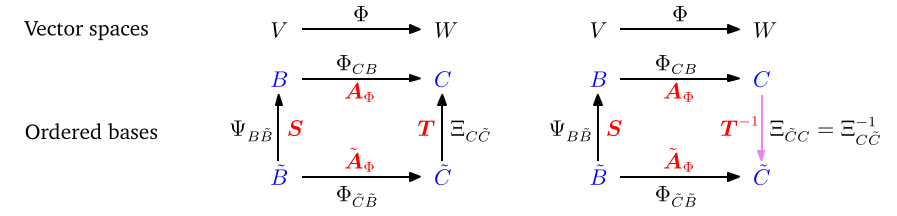
\includegraphics[width=10cm]{2}\\
\centering
\end{figure}\\
First we find the matrix representaion of the linear mapping $\Psi_{B\tilde{B}}:V\to V$ that 
maps coordinates with respect to the `new' basis $\tilde{B}$ onto the (unique) coordinates with respect 
to the `old' basis $B$ (in $V$). Then we use the transformation matrix $\bm{A}_\Phi$ of 
of $\Phi_{CB}:V\to W$ to map these coordinates onto the coordinates with respect to $C$ in $W$. 
Finally we use the inverse of the linear mapping $\Xi_{C\tilde{C}}:W\to W$ that maps the coordinates 
with respect to $\tilde{C}$ onto the coordinates with respect to $C$. Thus the linear mapping 
$\Phi_{\tilde{C}\tilde{B}}$ can be expressed as a composition of linear mappings (that involve the `old' basis):
\begin{equation*}
\Phi_{\tilde{C}\tilde{B}}=
\Xi^{-1}_{C\tilde{C}}\circ\Phi_{CB}\circ\Psi_{B\tilde{B}}
\end{equation*}
Concretely, $\Psi_{B\tilde{B}}=\text{id}_V$ and $\Xi_{C\tilde{C}}=\text{id}_W$; they are identity mappings
that map vectors onto themselves, but with respect to a different basis. 
(\textit{coordinate} expression of the vector changes, but the vector itself doesn't change)\\
\vspace{1mm}\\
Observe that the expression we derived
\begin{equation*}
\tilde{\bm{A}}_\Phi=\bm{T}^{-1}\bm{A}_\Phi\bm{S}
\end{equation*}
is simply the matrix representation of these mappings.\\
(next page)
\newpage
\noindent\textbf{Equivalence and Similarity}
\begin{itemize}
\item Two matrices $\bm{A},\tilde{\bm{A}}\in\mathbb{R}^{m\times n}$ are \textit{equivalent} if there 
exist regular/invertible matrices $\bm{S}\in\mathbb{R}^{n\times n}$ and $\bm{T}\in\mathbb{R}^{m\times m}$, 
such that $\tilde{\bm{A}}_\Phi=\bm{T}^{-1}\bm{A}_\Phi\bm{S}$. (both matrices map 
vectors from and to the same vector spaces, just using different basis vectors)
\item Two matrices $\bm{A},\tilde{\bm{A}}\in\mathbb{R}^{n\times n}$ are \textit{similar} if there
exists a regular matrix $\bm{S}\in\mathbb{R}^{n\times n}$ where $\tilde{\bm{A}}_\Phi=\bm{S}^{-1}\bm{A}_\Phi\bm{S}$.
(the identity mapping for changing bases in the initial and final vector spaces are the same)
\end{itemize}
Observe that similar matrices are always equivalent, but equivalent matrices are not necessarily similar.\\
\vspace{1mm}\\
\textbf{Matrix representation of Basis Changes}\\
Consider vector spaces $V,W,X$. We know that for linear mappings $\Phi:V\to W$ and $\Psi:W\to X$ the mapping
$\Psi\circ\Phi:V\to X$ is also linear.
With transformation matrices $\bm{A}_\Phi$ and $\bm{A}_\Psi$ of the corresponding mappings, the overall
transformation matrix is $\bm{A}_{\Psi\circ\Phi}=\bm{A}_\Psi\bm{A}_\Phi$. Now look at the 
matrices that represent basis changes from the perspectiveof composing linear mappings:
\begin{itemize}
\item$\bm{A}_\Phi$ is the transformation matrix of a linear mapping $\Phi_{CB}:V\to W$ with respect
to the bases $B,C$.
\item$\tilde{\bm{A}}_\Phi$ is the transformation matrix of the linear mapping $\Phi_{\tilde{C}\tilde{B}}:V\to W$ with respect
to the bases $\tilde{B},\tilde{C}$.
\item$\bm{S}$ is the transformation matrix of a linear mapping $\Psi_{B\tilde{B}}:V\to V$ (automorphism)
that represents $\tilde{B}$ in terms of $B$. Normally,
$\Psi=\text{id}_V$ is the identity mapping in $V$.
\item$\bm{T}$ is the transformation matrix of a linear mapping $\Xi_{C\tilde{C}}:W\to W$ (automorphism)
that represents $\tilde{C}$ in terms of $C$. Normally
$\Xi=\text{id}_W$ is the identity mapping in $W$.
\end{itemize}
(Informally) writing down the transformations just in terms of bases, one can intuitively see how
the derived matrix representation coincdes with each linear mapping:
\begin{align*}
\tilde{B}\to\tilde{C}&=\tilde{B}\to B\to C\to\tilde{C}\\
\tilde{\bm{A}}_\Phi&=\bm{T}^{-1}\bm{A}_\Phi\bm{S}
\end{align*}
\newpage

\subsection{Image and Kernel} %190724
\textbf{Definition}\\
For $\Phi:V\to W$, we define the \textit{kernel/null space}
\begin{equation*}
\ker(\Phi):=\Phi^{-1}(\mathbf{0}_W)=\{\bm{v}\in V:\Phi(\bm{v})=\mathbf{0}_W\}
\end{equation*}
and the \textit{image/range}
\begin{equation*}
\text{Im}(\Phi):=\Phi(V)=\{\bm{w}\in W|\exists\bm{v}\in V:\Phi(\bm{v})=\bm{w}\}
\end{equation*}
We also call $V$ and $W$ the \textit{domain} and \textit{codomain} of $\Phi$, respectively.\\
\vspace{1mm}\\
Intuitively, the kernel is the set of vectors $\bm{v}\in V$ that $\Phi$ maps onto the neutral element
$\mathbf{0}_W\in W$. The image is the set of vectors $\bm{w}\in W$ that can be
`reached' by $\Phi$ from any vector in $V$:
\begin{figure}[h]
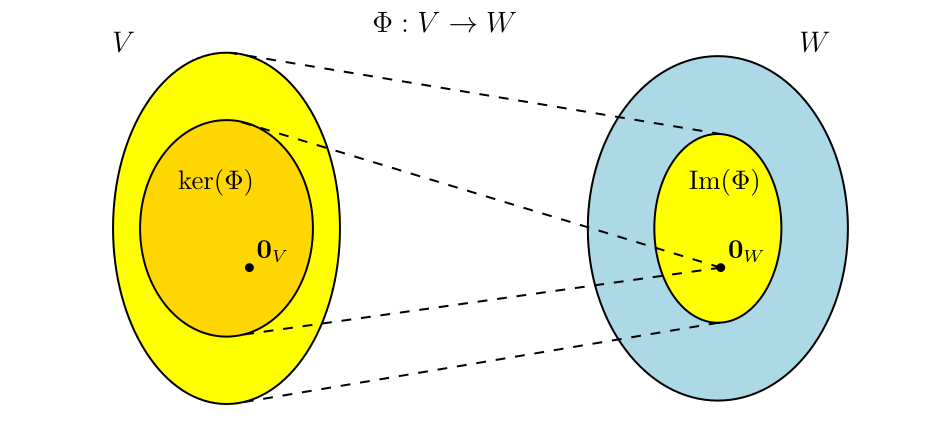
\includegraphics[width=10cm]{3}\\
\centering
\end{figure}\\
\textbf{Properties}\\
Consider a linear mapping $\Phi:V\to W$, where $V,W$ are vector spaces.
\begin{itemize}
\item It always holds that $\Phi(\mathbf{0}_V)=\mathbf{0}_W$ and therefore 
$\mathbf{0}_V\in\ker(\Phi)$. This also means the null space is never empty.
\item$\text{Im}(\Phi)\subseteq W$ is a subspace of $W$, and $\ker(\Phi)\subseteq V$ is a subspace of $V$.
\item$\Phi$ is injective (one-to-one) if and only if $\ker(\Phi)=\{\mathbf{0}\}$.
\end{itemize}
(next page)
\newpage
\noindent\textbf{Null Space and Column Space}\\
Consider $\bm{A}\in\mathbb{R}^{m\times n}$ and a linear mapping 
$\Phi:\mathbb{R}^n\to\mathbb{R}^m,x\mapsto\bm{A}x$.
\begin{itemize}
\item For $\bm{A=[a}_1,\ldots,\bm{a}_n]$, where $\bm{a}_i$ are the columns of $\bm{A}$, we obtain
\begin{align*}
\text{Im}(\Phi)&=\{\bm{Ax}:\bm{x}\in\mathbb{R}^n\}
=\left\{\sum^n_{i=1}x_i\bm{a}_i:x_1,\ldots,x_n\in\mathbb{R},\bm{a}_i\in\mathbb{R}^m\right\}\\
&=\text{span}[\bm{a}_1,\ldots,\bm{a}_n]\subseteq\mathbb{R}^m
\end{align*}
Essentially this means the image is the span of the columns of $\bm{A}$, also called the
\textit{column space}. Therefore, the column space (image) is a subspace of $\mathbb{R}^m$, 
where $m$ is the `height' of the matrix.
\item$\text{rk}(A)=\dim(\text{Im}(\Phi))$.
\item The kernel/null space $\ker(\Phi)$ is the general solution to the homogeneous system of linear
equations $\bm{Ax}=\mathbf{0}$; it captures all possible linear combinations of the elements in $\mathbb{R}^n$
that produce $\bm{0}\in\mathbb{R}^m$.
\item The kernel is a subspace of $\mathbb{R}^n$, where $n$ is the `width' of the matrix. 
\item The kernel can be used to determine whether/how a column can be expressed as a linear combination
of other columns.
\end{itemize}
\textbf{Example}: Consider
\begin{align*}
\Phi:\mathbb{R}^4\to\mathbb{R}^2,\quad\begin{bmatrix*}
x_1\\x_2\\x_3\\x_4
\end{bmatrix*}\mapsto\begin{bmatrix*}
1&2&-1&0\\1&0&0&1
\end{bmatrix*}\begin{bmatrix*}
x_1\\x_2\\x_3\\x_4
\end{bmatrix*}\\
=x_1\begin{bmatrix}1\\1\end{bmatrix}
+x_2\begin{bmatrix}2\\0\end{bmatrix}
+x_3\begin{bmatrix}-1\\0\end{bmatrix}
+x_4\begin{bmatrix}0\\1\end{bmatrix}
\end{align*}
We get the image from the span of the columns of the transformation matrix, also called the column space.
\begin{equation*}
\text{Im}(\Phi)=\text{span}[
\begin{bmatrix}1\\1\end{bmatrix},
\begin{bmatrix}2\\0\end{bmatrix},
\begin{bmatrix}-1\\0\end{bmatrix},
\begin{bmatrix}0\\1\end{bmatrix}]
\end{equation*}
To compute the kernel/null space of $\Phi$ we solve $\bm{Ax}=\mathbf{0}$, this can be done by Gaussian elimination:
\begin{equation*}
\begin{bmatrix*}
1&2&-1&0\\1&0&0&1
\end{bmatrix*}\rightsquigarrow\ldots\rightsquigarrow
\begin{bmatrix*}
1&0&0&1\\0&1&-1/2&-1/2
\end{bmatrix*}
\end{equation*}
which gives us (either by observation or with the Minus-1 Trick)
\begin{equation*}
\text{ker}(\Phi)=\text{span}[
\begin{bmatrix*}
0\\1/2\\1\\0
\end{bmatrix*},
\begin{bmatrix*}
-1\\1/2\\0\\1
\end{bmatrix*}]
\end{equation*}
(next page)
\newpage
\noindent\textbf{Rank-Nullity Theorem}\\
\textbf{Theorem:} \textit{For vector spaces $V,W$ and a linear mapping $\Phi:V\to W$ it 
holds that}
\begin{equation*}
\text{dim}(\text{ker}(\Phi))+\text{dim}(\text{Im}(\Phi))
=\text{dim}(V)
\end{equation*}
(also called the \textit{fundamental theorem of linear mappings)} This leads to the following consequences:
\begin{itemize}
\item If $\text{dim}(\text{Im}(\Phi))<\text{dim}(V)$, then $\text{ker}(\Phi)$ is non-trivial, 
meaning the kernel contains more than $\mathbf{0}_V$ and $\text{dim}(\text{ker}(\Phi))\geq1$.
\item If $\bm{A}_\Phi$ is a transformation matrix of $\Phi$ with respect to an ordered basis and 
$\text{dim}(\text{Im}(\Phi))<\text{dim}(V)$, then the system of linear equations $\bm{A}_\Phi\bm{x}=\mathbf{0}$
has infinitely many solutions.
\item If $\text{dim}(V)=\text{dim}(W)$, then the three-way equivalence
\begin{equation*}
\Phi\text{ is injective}\iff\Phi\text{ is surjective}\iff\Phi\text{ is bijective}
\end{equation*}
\end{itemize}
holds since $\text{Im}(\Phi)\subseteq W$ (and $\text{dim}(\text{Im}(\Phi))
=\text{dim}(V)$) (see (\ref{fundamentals:linear mappings})).
\newpage

\subsection{Affine Spaces} %210724
\textbf{Definition}\\
Let $V$ be a vector space, $\bm{x}_0\in V$ and $U\subseteq V$ a subspace. Then the subset
\begin{align*}
L&=\bm{x}_0+U:=\{\bm{x}_0+\bm{u}:\bm{u}\in U\}\\
&=\{\bm{v}\in V|\exists\bm{u}\in U:\bm{v}=\bm{x}_0+\bm{u}\}\subseteq V
\end{align*}
is called an \textit{affine subspace/linear manifold} of $V$. $U$ is called the \textit{direction or direction space},
and $\bm{x}_0$ is called the \textit{support point}. (Affine subspaces can also be referred to as 
\textit{hyperplanes}).\\
\vspace{1mm}\\
Note that the definition of an affine subspace excludes $\mathbf{0}$ if $\bm{x}_0\notin U$. 
Therefore an affine subspace is not a linear (vector) subspace of $V$ for $\bm{x}_0\notin U$. 
(due to lack of a neutral element)\\
\vspace{1mm}\\
\textbf{Subsets of Affine Spaces}\\
Consider two affine spaces $L=\bm{x}_0+U$
and $\tilde{L}=\tilde{\bm{x}}_0+\tilde{U}$ of a vector space $V$. 
Then $L\subseteq\tilde{L}$ if and only if $U\subseteq\tilde{U}$ and $\bm{x}_0-\tilde{\bm{x}}_0\in\tilde{U}$.\\
\vspace{1mm}\\
\textbf{Parametric representation}\\
Affine subspaces are often described by \textit{parameters}: Consider a $k$-dimensional
affine space $L=\bm{x}_0+U$ of $V$. If $(\bm{b}_1,\ldots,\bm{b}_k)$ is an ordered basis of $U$,
then every element $\bm{x}\in L$ can be uniquely described as
\begin{equation*}
\bm{x}=\bm{x}_0+\lambda_1\bm{b}_1+\ldots+
\lambda_k\bm{b}_k
\end{equation*}
where $\lambda_1,\ldots,\lambda_k\in\mathbb{R}$. This representation is called the \textit{parametric equation} 
of $L$ with directional vectors $\bm{b}_1,\ldots,\bm{b}_k$ and \textit{parameters} $\lambda_1,\ldots,\lambda_k$.
\\
(next page)
\newpage
\noindent\textbf{Examples of Affine Subspaces}
\begin{itemize}
\item One-dimensional affine subspaces are called \textit{lines}, and can be written parametrically as 
$\bm{y}=\bm{x}_0+\lambda_1\bm{b}_1$, where $\lambda\in\mathbb{R}$ and 
$U=\text{span}[\bm{b}_1]\subseteq\mathbb{R}^n$ is a one dimensional subspace of $\mathbb{R}^n$. Illustrated:
\begin{figure}[h]
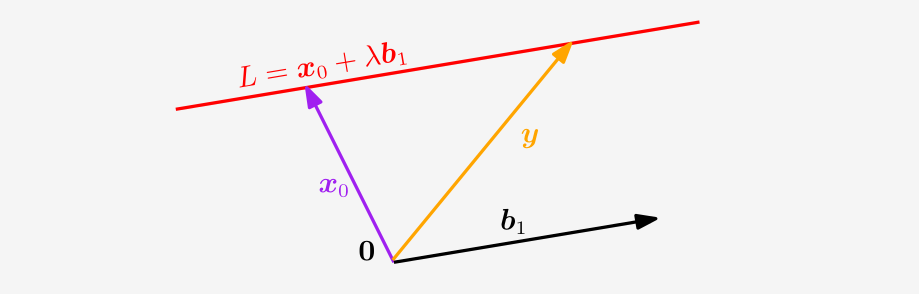
\includegraphics[width=10cm]{4}\\
\centering
\end{figure}
\item Two-dimensional affine subspaces of $\mathbb{R}^n$ are called \textit{planes}, with parametric equation
$\bm{y}=\bm{x}_0+\lambda_1\bm{b}_1+\lambda_2\bm{b}_2$, where $\lambda_1,\lambda_2\in\mathbb{R}$ 
and $U=\text{span}[\bm{b}_1,\bm{b}_2]\subseteq\mathbb{R}^n$.
\item In $\mathbb{R}^n$, the $(n-1)$-dimensional affine subspaces are called \textit{hyperplanes}, 
with parametric equation $\bm{y}=\bm{x}_0+\sum^{n-1}_{i=1}\lambda_i\bm{b}_i$, where
$\bm{b}_1,\ldots\bm{b}_{n-1}$ form a basis of an $(n-1)$-dimensional subspace $U$ of $\mathbb{R}^n$. (in $\mathbb{R}^2$, a line is a hyperplane; 
in $\mathbb{R}^3$, a plane is a hyperplane.
\end{itemize}
\textbf{Inhomogeneous systems of linear equations and affine subspaces}\\
For $\bm{A}\in\mathbb{R}^{m\times n}$ and $\bm{x}\in\mathbb{R}^m$, the solution of the system of 
linear equations $\bm{A\lambda}=\bm{x}$ is either the empty set or an affine subspace of $\mathbb{R}^n$ of 
dimension $n-\text{rk}(A)$; the solution of the linear equation 
$\lambda_1\bm{b}_1+\ldots+\lambda_n\bm{b}_n=\bm{x}$, where $(\lambda_1,\ldots,\lambda_n)\neq(0,\ldots,0)$, 
is a hyperplane in $\mathbb{R}^n$. (I assume solutions for one-to-one 
mappings are also affine spaces with direction 
$\{\mathbf{0}\}$ and support vector equal to the solution).\\
\vspace{1mm}\\
Viewed in another way, every $k$-dimensional affine subspace is the solution to an inhomogeneous system 
$\bm{Ax}=\bm{b}$, where $\bm{A}\in\mathbb{R}^{m\times n},\bm{b}\in\mathbb{R}^m$ and $\text{rk}(A)=n-k$. 
(The solution to $\bm{Ax}=\mathbf{0}$ can also be thought of as a special affine subspace with support 
point $\bm{x}_0=\mathbf{0}$.)\\
(next page)
\newpage
\noindent\textbf{Affine Mappings}\\
\textbf{Definition}\\
For two vector spaces $V,W$, a linear mapping $\Phi:V\to W$, and $\bm{a}\in W$, the mapping
\begin{align*}
\phi:&V\to W\\
&\bm{x}\mapsto\bm{a}+\Phi(\bm{x})
\end{align*}
is an \textit{affine mapping} from $V$ to $W$. The vector $\bm{a}$ is called the 
\textit{translation vector} of $\phi$.
Note that
\begin{itemize}
\item Every affine mapping $\phi:V\to W$ is also a composition of linear mapping
$\Phi:V\to W$ and a translation $\tau:W\to W$ in $W$, such that $\phi=\tau\circ\Phi$. The mappings $\Phi$ and $\tau$
are uniquely determined.
\item The composition $\phi'\circ\phi$ of affine mappings
$\phi:V\to W,\,\phi':W\to X$ is affine.
\item If $\phi$ is bijective, affine mappings keep the geometric structure invariant. They also
preserve the dimension and parallelism.
\end{itemize}
\newpage

\section{Analytic Geometry}
\subsection{Norms} %230724
\label{analytic geometry:norms}
\textbf{Definition}\\
A \textit{norm} on a vector space $V$ is a function
\begin{align*}
||\cdot||:&V\to \mathbb{R}\\
&\bm{x}\mapsto||\bm{x}||
\end{align*}
which assigns each vector $\bm{x}$ its \textit{length} $||\bm{x}||\in\mathbb{R}$, such that for all 
$\lambda\in\mathbb{R}$ and $\bm{x},\bm{y}\in V$ the following hold:
\begin{itemize}
\item\textit{Absolutely homogeneous}: $||\lambda \bm{x}||=|\lambda|\,||\bm{x}||$
\item\textit{Triangle inequality}: $||\bm{x}+\bm{y}||\leq||\bm{x}||+||\bm{y}||$\begin{figure}[h]
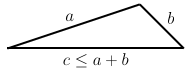
\includegraphics[width=4cm]{5}\\
\centering
\end{figure}
\item\textit{Positive definite}: $||\bm{x}||\geq0$ and $||\bm{x}||=0\implies\bm{x}=\mathbf{0}$
\end{itemize}
\textbf{Example}: Manhattan and Euclidean Norm\\
The \textit{Manhattan Norm} on $\mathbb{R}^n$ is defined for $\bm{x}\in\mathbb{R}^n$ as 
\begin{equation*}
||\bm{x}||_1:=\sum^{n}_{i=1}|x_i|
\end{equation*}
where $|\cdot|$ is the absolute value.
The \textit{Euclidean norm} for $\bm{x}\in\mathbb{R}^n$ is defined as
\begin{equation*}
||\bm{x}||_2:=\sqrt{\sum^n_{i=1}x_i^2}=\sqrt{\bm{x}^T\bm{x}}
\end{equation*}
giving us the \textit{Euclidean distance} of $\bm{x}$ from the origin. The Euclidean norm is also 
called the $\ell_2$ norm.
\begin{figure}[h]
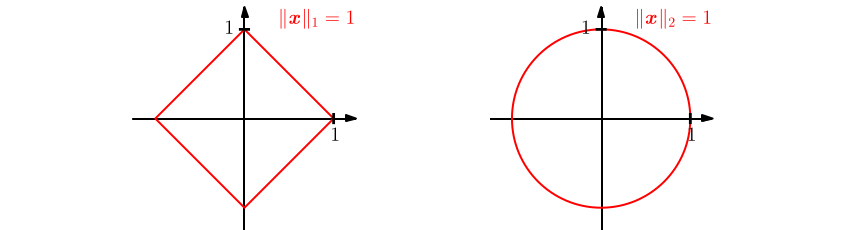
\includegraphics[width=10cm]{6}\\
\centering
Vectors $\bm{x}\in\mathbb{R}^2$ with $||\bm{x}||_1=1$ (left) and $||\bm{x}||_2=1$ (right)
\end{figure}\\
Generally the Euclidean norm is used by default if not stated otherwise.
\newpage

\subsection{Inner Products} %230724
\textbf{Dot Product}\\
The \textit{scalar/dot product} in $\mathbb{R}^n$ is given by
\begin{equation*}
\bm{x}^T\bm{y}=\sum^n_{i=1}x_iy_i
\end{equation*}
The Dot product is a type of inner product, but inner products are actually more general concepts with specific properties.\\
\vspace{1mm}\\
\textbf{General Inner Products}\\
Linear mappings can be rearranged with respect to addition and multiplication with a scalar. 
A \textit{bilinear mapping} $\Omega$ is a mapping with two arguments, and is linear in each argument; for instance
considering a vector space $V$, it holds that for all
$\bm{x},\bm{y},\bm{z}\in V,\,\lambda,\psi\in\mathbb{R}$
that
\begin{align*}
\Omega(\lambda\bm{x}+\psi\bm{y},\bm{z})&=\lambda\Omega(\bm{x},\bm{z})+\psi\Omega(\bm{y},\bm{z})\\
\Omega(\bm{x},\lambda\bm{y}+\psi\bm{z})&=\lambda\Omega(\bm{x},\bm{y})+\psi\Omega(\bm{x},\bm{z})
\end{align*}
point here is that $\Omega$ is linear in both arguments.\\
\vspace{1mm}\\
\textbf{Definition: Symmetric, Positive definite}\\
Let $V$ be a vector space and $\Omega:V\times V\to\mathbb{R}$ be a bilinear mapping that takes two
vectors and maps them onto a real number. Then
\begin{itemize}
\item$\Omega$ is called \textit{symmetric} if $\Omega(\bm{x},\bm{y})=\Omega(\bm{y},\bm{x})$ for all
$\bm{x},\bm{y}\in V$; essentially the order of the arguments does not matter.
\item$\Omega$ is called \textit{positive definite} if
\begin{equation*}
\forall\bm{x}\in V\backslash\{\mathbf{0}\}:\Omega(\bm{x},\bm{x})>0,\quad\Omega(\bm{0},\bm{0})=0
\end{equation*}
\end{itemize}
\textbf{Definition: Inner Product, Inner Product Space}\\
Let $V$ be a vector space and $\Omega:V\times V\to\mathbb{R}$ be a bilinear mapping that takes two vectors
and maps them onto a real number. Then
\begin{itemize}
\item A positive definite, symmetric bilinear mapping $\Omega:V\times V\to\mathbb{R}$ is called an
\textit{inner product} on $V$, typically written
$\langle x,y\rangle$ instead of $\Omega(x,y)$.
\item The pair $(V,\langle\cdot,\cdot\rangle)$ is called an \textit{inner product space} or 
(real) \textit{vector space with inner product}. If the inner product is the dot product, we call 
$(V,\langle\cdot,\cdot\rangle)$ a \textit{Euclidean vector space}.
\end{itemize}
\newpage

\subsection{Symmetric, Positive Definite Matrices} %230724
Consider an $n$-dimensional vector space $V$ with an inner product $\langle\cdot,\cdot\rangle:V\times V\to
\mathbb{R}$ and an ordered basis $B=(\bm{b}_1,\ldots,\bm{b}_n)$ of $V$. 
Since any vectors $\bm{x},\bm{y}\in V$ can be written as linear combinations of the basis vectors
such that 
\begin{equation*}
\bm{x}=\sum^n_{i=1}\psi_i\bm{b}_i\in V,\quad\text{and}\quad\bm{y}
=\sum^n_{j=1}\lambda_j\bm{b}_j\in V
\end{equation*}
for suitable $\psi_i,\lambda_j\in\mathbb{R}$, due to the bilinearity of the inner product it holds that for 
all $\bm{x},\bm{y}\in V$ that
\begin{equation*}
\langle\bm{x},\bm{y}\rangle=\left\langle\sum^n_{i=1}\psi_i\bm{b}_i,\sum^n_{j=1}\lambda_j\bm{b}_j\right\rangle
=\sum^n_{i=1}\sum^n_{j=1}\psi_i\langle\bm{b}_i,\bm{b}_j\rangle\lambda_j
=\hat{\bm{x}}^T\bm{A}\hat{\bm{y}}
\end{equation*}
where $A_{ij}:=\langle\bm{b}_i,\bm{b}_j\rangle$ and $\hat{\bm{x}}$ and $\hat{\bm{y}}$ are the coordinates
of $\bm{x}$ and $\bm{y}$ with respect to the basis $B$.\\
\vspace{1mm}\\
This implies that the inner product $\langle\cdot,\cdot\rangle$ is uniquely determined through $\bm{A}$. 
The symmetry of the inner product also means that $\bm{A}$ is symmetric. Furthermore, the 
positive definiteness of the inner product implies that
\begin{equation*}
\forall\bm{x}\in V\backslash\{\bm{0}\}:\bm{x}^T\bm{Ax}>0
\end{equation*}
\textbf{Definition}\\
Following from the above reasoning, we define a symmetric matrix $\bm{A}\in\mathbb{R}^{n\times n}$ that
satisfies
\begin{equation*}
\forall\bm{x}\in V\backslash\{\bm{0}\}:\bm{x}^T\bm{Ax}>0
\end{equation*}
to be \textit{symmetric, positive definite} or just \textit{positive definite}. If only $\geq$ holds 
then $\bm{A}$ is called \textit{symmetric, positive semidefinite}.\\
\vspace{1mm}\\
\textbf{Example}: Considering the matrices
\begin{equation*}
\bm{A}_1=\begin{bmatrix}
9&6\\6&5
\end{bmatrix},\quad\begin{bmatrix}
9&6\\6&3
\end{bmatrix}
\end{equation*}
$\bm{A}_1$ is positive definite because it is symmetric and for all $\bm{x}\in V\backslash\{\bm{0}\}$
\begin{align*}
\bm{x}^T\bm{A}_1\bm{x}&=\begin{bmatrix}x_1&x_2\end{bmatrix}\begin{bmatrix}9&6\\6&5\end{bmatrix}
\begin{bmatrix}x_1\\x_2\end{bmatrix}\\
&=9x_1^2+12x_1x_2+5x_2^2=(3x_1+2x_2)^2+x_2^2)>0
\end{align*}
While $\bm{A}_2$ is symmetric but not positive definite because
\begin{equation*}
\bm{x}^T\bm{A}_2\bm{x}
=9x_1^2+12x_1x_2+3x_2^2=(3x_1+2x_2)^2-x_2^2)
\end{equation*}
which isn't always greater than 0 for all $\bm{x}\in V\backslash\{\bm{0}\}$.\\
(next page)
\newpage
\noindent\textbf{Significance of symmetric positive definite matrices}\\
If $\bm{A}\in\mathbb{R}^{n\times n}$ is symmetric, positive definite, then
\begin{equation*}
\langle\bm{x},\bm{y}\rangle=\hat{\bm{x}}^T\bm{A}\tilde{\bm{y}}
\end{equation*}
defines an inner product with respect to an ordered basis $B$, where $\hat{\bm{x}}$ and $\hat{\bm{y}}$ are 
the coordinate representations of $\bm{x},\bm{y}\in V$ with respect to $B$.\\
\vspace{1mm}\\
\textbf{Theorem 3.5}: \textit{For a real-valued, finite-dimensional vector space $V$ and an ordered
basis $B$ of $V$, it holds that $\langle\cdot,\cdot\rangle:V\times V\to\mathbb{R}$ is an inner product if and
only if there exists a symmetric, positive definite matrix $\bm{A}\in\mathbb{R}^{n\times n}$ with}
\begin{equation*}
\langle\bm{x},\bm{y}\rangle=\hat{\bm{x}}^T\bm{A}\tilde{\bm{y}}
\end{equation*}
If $A\in\mathbb{R}^{n\times n}$ is symmetric and positive definite, the following properties hold:
\begin{itemize}
\item The null space/kernel of $\bm{A}$ consists only of $\bm{0}$ because $\bm{x}^T\bm{Ax}>0$ for all
$\bm{x}\neq\bm{0}$. This implies that $\bm{Ax}\neq\bm{0}$ if $\bm{x}\neq\bm{0}$.
\item The diagonal elements $a_{ii}$ of $\bm{A}$ are positive because $a_{ii}=\bm{e}_i^T\bm{A}\bm{e}_i>0$,
where $\bm{e}_i$ is the $i$-th vector of the standard basis in $\mathbb{R}^n$. (Alternatively, see that $\bm{A}$
is just made up of the inner product of different combinations of the basis vectors, where the diagonal only has
inner products between each basis vector and itself; the positive definite requirement of the inner product
therefore means that the diagonal will be positive.)
\end{itemize}
\newpage

\subsection{Cauchy-Schwarz Inequality} %240724
For an inner product vector space ($V,\langle\cdot,\cdot\rangle$) the induced norm satisfies the 
\textit{Cauchy-Schwarz inequality}
\begin{equation*}
|\langle\bm{x},\bm{y}\rangle|\leq||\bm{x}||\,||\bm{y}||
\end{equation*}
The equality only holds if $\bm{x}$ and $\bm{y}$ are linearly dependent.\\
\vspace{1mm}\\
\textbf{Proof}\\
Let $V$ be a vector space over the real or complex field $F$, and let $\bm{x},\bm{y}\in V$. First we show that
$|\langle\bm{x},\bm{y}\rangle|^2=\langle\bm{x},\bm{x}\rangle\,\langle\bm{y},\bm{y}\rangle$
if $\bm{y}=a\bm{x}$ for some $a\in F$ (linearly dependent).
Then we show $|\langle\bm{x},\bm{y}\rangle|^2<\langle\bm{x},\bm{x}\rangle\,\langle\bm{y},\bm{y}\rangle$ if 
$\bm{y}\neq a\bm{x}$ for all $a\in F$ (linearly independent).\\
\vspace{1mm}\\
If $\bm{y}=a\bm{x}$ for some $a\in F$
\begin{align*}
|\langle\bm{x},\bm{y}\rangle|^2&=|\langle\bm{x},a\bm{x}\rangle|^2\\
&=|a\langle\bm{x},\bm{x}\rangle|^2\quad\text{(linearity)}\\
&=|a|^2\langle\bm{x},\bm{x}\rangle^2
\end{align*}
similarly it follows that
\begin{align*}
\langle\bm{x},\bm{x}\rangle\langle\bm{y},\bm{y}\rangle
&=\langle\bm{x},\bm{x}\rangle\langle a\bm{x},a\bm{x}\rangle\\
&=\langle\bm{x},\bm{x}\rangle\,a^2\langle\bm{x},\bm{x}\rangle\\
&=|a|^2\langle\bm{x},\bm{x}\rangle^2
\end{align*}
giving us $|\langle\bm{x},\bm{y}\rangle|^2=\langle\bm{x},\bm{x}\rangle\,\langle\bm{y},\bm{y}\rangle$
if $\bm{y}=a\bm{x}$ for some $a\in F$ (linearly dependent). Now considering the case where
$\bm{y}\neq a\bm{x}$ for all $a\in F$; it is implied that $\bm{y}\neq0$ (because of $a$) and that therefore
$\langle\bm{y},\bm{y}\rangle\neq0$. We can also say that
for all $a\in F$, $\langle\bm{x}-a\bm{y},\bm{x}-a\bm{y}\rangle>0$. Now we expand:
\begin{align*}
\langle\bm{x}-a\bm{y},\bm{x}-a\bm{y}\rangle
&=\langle\bm{x},\bm{x}-a\bm{y}\rangle
-a\langle\bm{y},\bm{x}-a\bm{y}\rangle\\
&=\langle\bm{x},\bm{x}\rangle-a\langle\bm{x},\bm{y}\rangle
-a\langle\bm{y},\bm{x}\rangle
+a^2\langle\bm{y},\bm{y}\rangle
\end{align*}
Choosing $a=\frac{\langle\bm{x},\bm{y}\rangle}{\langle\bm{y},\bm{y}\rangle}$:
\begin{align*}
\langle\bm{x}-a\bm{y},\bm{x}-a\bm{y}\rangle
&=\langle\bm{x},\bm{x}\rangle-\frac{\langle\bm{x},\bm{y}\rangle}{\langle\bm{y},\bm{y}\rangle}\langle\bm{x},\bm{y}\rangle
-\frac{\langle\bm{x},\bm{y}\rangle}{\langle\bm{y},\bm{y}\rangle}\langle\bm{y},\bm{x}\rangle
+\frac{\langle\bm{x},\bm{y}\rangle^2}{\langle\bm{y},\bm{y}\rangle^2}\langle\bm{y},\bm{y}\rangle\\
&=\langle\bm{x},\bm{x}\rangle-\frac{\langle\bm{x},\bm{y}\rangle\langle\bm{y},\bm{x}\rangle}{\langle\bm{y},\bm{y}\rangle}
\end{align*}
(next page)
\newpage
\noindent Since we have $\langle\bm{x}-a\bm{y},\bm{x}-a\bm{y}\rangle>0$ and
\begin{equation*}
\langle\bm{x}-a\bm{y},\bm{x}-a\bm{y}\rangle=
\langle\bm{x},\bm{x}\rangle-
\frac{\langle\bm{x},\bm{y}\rangle\langle\bm{y},\bm{x}\rangle}{\langle\bm{y},\bm{y}\rangle}
\end{equation*}
we have the inequality 
\begin{align*}
\langle\bm{x},\bm{x}\rangle-
\frac{\langle\bm{x},\bm{y}\rangle\langle\bm{y},\bm{x}\rangle}{\langle\bm{y},\bm{y}\rangle}&>0\\
\langle\bm{x},\bm{x}\rangle\langle\bm{y},\bm{y}\rangle-
\langle\bm{x},\bm{y}\rangle\langle\bm{y},\bm{x}\rangle&>0\\
|\langle\bm{x},\bm{y}\rangle|^2&<\langle\bm{x},\bm{x}\rangle\langle\bm{y},\bm{y}\rangle
\end{align*}
where $\bm{y}\neq a\bm{x}$ for all $a\in F$.\\
\vspace{1mm}\\
Therefore the inequality 
\begin{equation*}
|\langle\bm{x},\bm{y}\rangle|^2\leq\langle\bm{x},\bm{x}\rangle\langle\bm{y},\bm{y}\rangle
\end{equation*}
holds for all $\bm{x},\bm{y}\in V$, with the equality holding only if they are linearly dependent.\\
\vspace{1mm}\\
Since the norm is induced by the inner product
\begin{equation*}
||\bm{x}||:=\sqrt{\langle\bm{x},\bm{x}\rangle}
\end{equation*}
we can also say
\begin{align*}
|\langle\bm{x},\bm{y}\rangle|^2&\leq||\bm{x}||^2||\bm{y}||^2\\
|\langle\bm{x},\bm{y}\rangle|&\leq||\bm{x}||\,||\bm{y}||
\end{align*}
\newpage

\subsection{Lengths and Distances} %240724
Inner products and norms are closely related in the sense that any inner product induces a norm, which represent
the length of a vector:
\begin{equation*}
||\bm{x}||:=\sqrt{\langle\bm{x},\bm{x}\rangle}
\end{equation*}
Different inner products therefore lead to different norms---different representations of the length
of a vector. Note however that not every norm is induced by an inner product 
(take the Manhattan norm for instance).\\
\vspace{1mm}\\
\textbf{Distance and Metric}\\
Considering an inner product space $(V,\langle\cdot,\cdot\rangle)$, 
\begin{equation*}
d(\bm{x},\bm{y}):=||\bm{x}-\bm{y}||=\sqrt{\langle\bm{x}-\bm{y},\bm{x}-\bm{y}\rangle}
\end{equation*}
is called the \textit{distance} between $\bm{x}$ and $\bm{y}$ for $\bm{x},\bm{y}\in V$. If
the dot product is used as the inner product, then the distance is called \textit{Euclidean distance}.\\
\vspace{1mm}\\
The mapping 
\begin{align*}
d:V\times V&\to\mathbb{R}\\
(\bm{x},\bm{y})&\mapsto d(\bm{x},\bm{y})
\end{align*}
is called a metric. (remember that the distance between vectors does not require an inner product; 
a norm is sufficient, but that an inner product, when defined, would induce a norm).\\
\vspace{1mm}\\
A metric $d$ satisfies the following:
\begin{enumerate}
\item$d$ is \textit{positive definite}, meaning $d(\bm{x},\bm{y})\geq0$ for all $\bm{x},\bm{y}\in V$
and $d(\bm{x},\bm{y})=0\iff\bm{x}=\bm{y}$.
\item$d$ is \textit{symmetric}, meaning $d(\bm{x},\bm{y})=d(\bm{y},\bm{x})$ for all $\bm{x},\bm{y}\in V$.
\item\textit{Triangle inequality}: $d(\bm{x},\bm{z})\leq
d(\bm{x},\bm{y})+d(\bm{y},\bm{z})$ for
all $\bm{x},\bm{y},\bm{z}\in V$.
\end{enumerate}
At first glance the properties of inner products and metrics appear similar. Note however that the 
properties of metrics come from those of norms rather than inner products (see (\ref{analytic geometry:norms})). 
Also notice that similar inputs will result in a small metric but not inner product.
\newpage

\subsection{Angles and Orthogonality} %240724
\textbf{Angle}\\
Inner products also capture the geometry of a vector space by defining the angle $\omega$ between 
two vectors. Using the Cauchy-Schwarz inequality, assuming that $\bm{x}\neq\bm{0},\bm{y}\neq\bm{0}$,
\begin{align*}
|\langle\bm{x},&\bm{y}\rangle|\leq||\bm{x}||\,||\bm{y}||\\
&\frac{|\langle\bm{x},\bm{y}\rangle|}{||\bm{x}||\,||\bm{y}||}\leq1\\
-1\leq&\frac{\langle\bm{x},\bm{y}\rangle}{||\bm{x}||\,||\bm{y}||}\leq1
\end{align*}
Thus there exists a unique $\omega\in[0,\pi]$, with
\begin{figure}[h]
\begin{equation*}
\cos\omega=\frac{\langle\bm{x},\bm{y}\rangle}{||\bm{x}||\,||\bm{y}||}
\end{equation*}
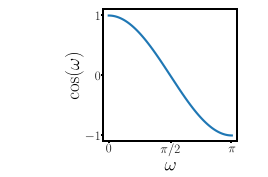
\includegraphics[width=6cm]{7}\\
\centering
\end{figure}\\
Each value in $[-1,1]$ corresponds to a unique $\omega$; the number $\omega$ is the \textit{angle} 
between the vectors $\bm{x}$ and $\bm{y}$. Intuitively, 
the angle between two vectors tells us how similar their orientations are. 
(For instance, using the dot product, the angle between $\bm{x}$ and $\bm{y}=4\bm{x}$ is 0.)\\
(next page)
\newpage
\noindent\textbf{Orthogonality}\\
The \textit{angle} $\omega$ in
\begin{equation*}
\cos\omega=\frac{\langle\bm{x},\bm{y}\rangle}{||\bm{x}||\,||\bm{y}||}
\end{equation*}
can be intuitively seen as a measure of how similar the orientation between two vectors are.
(The angle between a vector and itself is 0, for instance.)\\
\vspace{1mm}\\
\textbf{Definition}\\
Two vectors $\bm{x}$ and $\bm{y}$ are \textit{orthogonal} if and only if $\langle\bm{x},\bm{y}\rangle=0$,
written as $\bm{x}\perp\bm{y}$. If additionally $||\bm{x}||=1=||\bm{y}||$ (unit vectors), then
$\bm{x}$ and $\bm{y}$ are \textit{orthonormal}. (Notice that the $\bm{0}$-vector is orthogonal to every vector in
the vector space.)\\
\vspace{1mm}\\
Orthogonality is the generalisation of the concept of perpendicularity to bilinear forms that do
not have to be the dot product. Geometrically, one can think of orthogonal vectors as having a right
angle with respect to a \textit{specific} inner product.\\
\vspace{1mm}\\
\textbf{Example}\\
Consider two vectors $\bm{x}=[1,1]^T$,$\bm{y}=[-1,1]^T\in\mathbb{R}^2$. We are interested in determining the 
angle $\omega$ between them using two different inner products. Using the dot product as the
inner product yields an angle $\omega$ between $\bm{x}$ and $\bm{y}$ of $90^\circ$; in this case 
$\bm{x}\perp\bm{y}$. However, considering a different inner product
\begin{equation*}
\langle\bm{x},\bm{y}\rangle=\bm{x}^T\begin{bmatrix}
2&0\\0&1
\end{bmatrix}\bm{y}
\end{equation*}
we get a different angle $\omega$:
\begin{equation*}
\cos\omega=\frac{\langle\bm{x},\bm{y}\rangle}{||\bm{x}||\,||\bm{y}||}=-\frac{1}{3}\implies\omega\approx1.91\,
\text{rad}\approx109.5^\circ
\end{equation*}
\newpage

\subsection{Orthogonal Matrices} %250724
\label{analytic geometry:orthogonal matrices}
\textbf{Definition}\\
A square matrix $\bm{A}\in\mathbb{R}^{n\times n}$ is an \textit{orthogonal matrix} if and only if its columns are
\textbf{orthonormal} so that 
\begin{equation*}
\bm{AA}^T=\bm{I}=\bm{A}^T\bm{A}
\end{equation*}
which implies that
\begin{equation*}
\bm{A}^{-1}=\bm{A}^T
\end{equation*}
meaning the inverse can be obtained by transposing the matrix.\\
\vspace{1mm}\\
\textbf{Side note (250724)}:\\
`Orthogonal matrices' suggests some general
inner product expansion involved in matrix multiplication. But notice that orthogonality between columns
only holds for the standard inner product (the dot product); for intuition, consider an inner product
\begin{equation*}
\langle\bm{x},\bm{y}\rangle=\bm{x}^T\bm{M}\bm{y}
\end{equation*}
we only have $\bm{A}=(\bm{e}_1,\ldots,\bm{e}_n)$ being orthonormal if 
\begin{equation*}
\forall i,j:
\langle\bm{e}_i,\bm{e}_j\rangle=\bm{e}_i^T\bm{M}\bm{e}_j
=\delta_{i,j}
\end{equation*}
where $\delta_{i,j}$ is the kronecker delta. Written compactly in matrix notation:
\begin{equation*}
\bm{A}^T\bm{MA}=\bm{I}
\end{equation*}
only for the standard inner product $\bm{M}=\bm{I}$ do we
obtain $\bm{A}^T\bm{A}$.\\
\vspace{1mm}\\
(A better understanding comes from a definition for orthogonality of linear transformations: 
\textit{On a finite-dimensional inner product space $(\mathbb{V},\langle\cdot,\cdot\rangle)$, 
a linear transformation $T:\mathbb{V}\to\mathbb{V}$ is said to be \textbf{orthogonal} if it preserves 
the inner product, that is, if $\langle T(x),T(y)\rangle=\langle\bm{x},\bm{y}\rangle$};
the definition $\bm{AA}^T=\bm{I}=\bm{A}^T\bm{A}$ comes from $\bm{A}$ being a matrix representation of such a
mapping (thus the added requirement of orthonormality)).\\
(next page)
\newpage
\noindent\textbf{Properties}\\
\textit{Transformations} by orthogonal matrices are special because the length of a vector $x$ is not
changed after the transformation. For the dot product we obtain 
(notice that orthogonality of $A$ depends on the choice of inner product)
\begin{equation*}
||\bm{Ax}||^2=(\bm{Ax})^T(\bm{Ax})=\bm{x}^T\bm{A}^T\bm{Ax}
=\bm{x}^T\bm{Ix}=\bm{x}^T\bm{x}=||\bm{x}||^2
\end{equation*}
The angle, as measured by the inner product, is also unchanged upon transformation by an orthogonal matrix; 
assuming the dot product as the inner product:
\begin{equation*}
\cos\omega=\frac{(\bm{Ax}^T)(\bm{Ay})}{||\bm{Ax}||\,||\bm{Ay}||}
=\frac{\bm{x}^T\bm{A}^T\bm{Ay}}{\sqrt{\bm{x}^T\bm{A}^T\bm{Ax}\bm{y}^T\bm{A}^T\bm{Ay}}}
=\frac{\bm{x}^T\bm{y}}{||\bm{x}||\,||\bm{y}||}
\end{equation*}
Orthogonal matrices therefore preserve both angles and distances. 
\newpage

\subsection{Orthonormal Basis and Complement} %260724
\textbf{Orthogonal Basis}\\
Considering an $n$-dimensional vector space $V$ and a basis $\{\bm{b}_1,\ldots,\bm{b}_n\}$ of $V$. If
\begin{align*}
\langle\bm{b}_i,\bm{b}_j\rangle&=0\quad\text{(for $i\neq j$)}\\
\langle\bm{b}_i,\bm{b}_i\rangle&=1
\end{align*}
for all $i,j=1,\ldots,n$ then the basis is called an \textit{orthonormal basis (ONB)}. If only 
$\langle\bm{b}_i,\bm{b}_j\rangle=0$ for $i\neq j$, then the basis is called an \textit{orthogonal basis}.\\
\vspace{1mm}\\
\textbf{Orthogonal Complement}\\
Consider a $D$-dimensional vector space $V$ and an $M$-dimenstional subspace $U\in V$. Then its 
\textit{orthogonal complement} $U^\perp$ is a $(D-M)$-dimensional subspace of $V$ and contains all vectors in
$V$ that are orthogonal to every vector in $U$.\\
\vspace{1mm}\\
Since $U\cap U^\perp=\{\bm{0}\}$ any vector $\bm{x}\in V$ can be uniquely decomposed into
\begin{equation*}
\bm{x}=\sum^M_{m=1}\lambda_m\bm{b}_m+\sum^{D-M}_{j=1}\psi_j\bm{b}^\perp_j,\quad
\lambda_m,\psi_j\in\mathbb{R}
\end{equation*}
where $(\bm{b}_1,\ldots,\bm{b}_M)$ is basis of $U$ and 
$(\bm{b}^\perp_1,\ldots,\bm{b}^\perp_{D-M})$
is a basis of $U^\perp$.\\
\vspace{1mm}\\
Orthogonal complements can be used to describe hyperplanes in $n$-dimensional vector/affine spaces.
For instance consider a three dimensional vector space; a plane $U$ in this space can be described 
by a vector $w$ orthogonal to the it (called the \textit{normal} vector of $U$). The vector $w$ with $||w||=1$
is the basis vector of $U^T$.
\newpage

\subsection{Inner Product of Functions}%270724
We can think of a vector $\bm{x}\in\mathbb{R}^n$ as a function with $n$ function values (outputs). The concept
of an inner product can then be generalised to vectors with an infinite number of entries (countably infinite) 
and also continuous-valued functions (uncountably infinite). The sum over individual components of vector
can be expressed as an integral.\\
\vspace{1mm}\\
An inner product of two functions $u:\mathbb{R}\to\mathbb{R}$ and $v:\mathbb{R}\to\mathbb{R}$ can be defined as
the definite integral
\begin{equation*}
\langle u,v\rangle:=\int_a^bu(x)v(x)dx
\end{equation*}
for lower and upper limits $a,b<\infty$. As with usual inner products, we can define norms and orthogonality
from the inner product. (more mathematically precise definitions require real and functional analysis)\\
\vspace{1mm}\\
\textbf{Example}\\
If we choose $u=\sin(x)$ and $v=\cos(x)$, the integrand $f(x)=u(x)v(x)$ is odd. Therefore the integral
over the limits $a=-\pi,\,b=\pi$ of $f$ evaluates to 0---$\sin$ and $\cos$ are orthogonal functions.\\
\vspace{1mm}\\
Also notice that the collection of functions
\begin{equation*}
\{1,\cos(x),\cos(2x),\cos(3x),\ldots\}
\end{equation*}
is orthogonal if we integrate over $-\pi$ to $\pi$ meaning any pair of functions are orthogonal. Projection
of functions onto this subspace is the fundamental idea
behind Fourier series.
\newpage

\subsection{Orthogonal Projections I}%270724
\textbf{Projection}\\
Let $V$ be a vector space and $U\subseteq V$ a subspace of $V$. A linear mapping 
$\pi:V\to U$ is called a \textit{projection} if $\pi^2=\pi\circ\pi=\pi$.\\
\vspace{1mm}\\
Linear mappings can be expressed as matrices; correspondingly, projections can be expressed as
\textit{projection matrices} $\bm{P}_\pi$, which 
exhibit the property $\bm{P}_\pi^2=\bm{P}_\pi$.\\
\vspace{1mm}\\
\textbf{Orthogonal projection onto one-dimensional subspaces}\\
Consider a one-dimensional subspace (a line) through the origin with basis vector $\bm{b}\in\mathbb{R}^n$. 
Say the line is a one-dimensional subspace $U\subseteq\mathbb{R}^n$ spanned by $\bm{b}$.
When we project $\bm{x}\in\mathbb{R}^n$ onto $U$, we are seeking the vector $\pi_U(\bm{x})\in U$ that is 
closest to $\bm{x}$.
\begin{figure}[h]
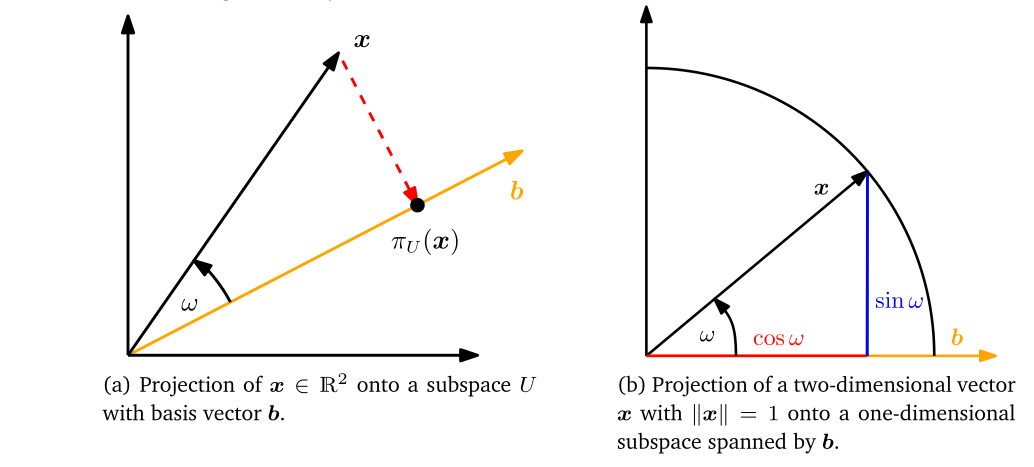
\includegraphics[width=10cm]{8}\\
\centering
\end{figure}\\
We can characterise the properties of the projection $\pi_U(\bm{x})$ as the following:
\begin{itemize}
\item The projection $\pi_U(\bm{x})$ is closest to $\bm{x}$, where `closest' implies the distance
$||\bm{x}-\pi_U(\bm{x})||$ is minimal. It follows that the segment $\pi_U(\bm{x})-\bm{x}$
from $\pi_U(\bm{x})$ to $\bm{x}$ is orthogonal to $U$ and therefore the basis vector $\bm{b}$ of $U$.
The orthogonality condition yields $\langle\pi_U(\bm{x})-\bm{x},\bm{b}\rangle=0$ since angles between
vectors are defined by the inner product.
\item The projection $\pi_U(\bm{x})$ of $\bm{x}$ onto $U$ must be an element of $U$ and therefore a multiple
of the basis vector $\bm{b}$ that spans $U$. Hence $\pi_U(\bm{x})=\lambda\bm{b}$ for some $\lambda\in\mathbb{R}$.
\end{itemize}
(next page)
\newpage
\noindent\textbf{Deriving the projection}
\begin{enumerate}
\item\textbf{Determining the coordinate of projection $\lambda$}\\
The orthogonality condition yields
\begin{equation*}
\langle\bm{x}-\pi_U(\bm{x}),\bm{b}\rangle=0
\iff\langle\bm{x}-\lambda\bm{b},\bm{b}\rangle=0
\end{equation*}
Exploiting the bilinearity of the inner product:
\begin{equation*}
\langle\bm{x},\bm{b}\rangle-\lambda\langle\bm{b},\bm{b}\rangle=0\iff
\lambda=\frac{\langle\bm{x},\bm{b}\rangle}{\langle\bm{b},\bm{b}\rangle}=
\frac{\langle\bm{b},\bm{x}\rangle}{||\bm{b}||^2}
\end{equation*}
If we choose $\langle\cdot,\cdot\rangle$ to be the dot product,
\begin{equation*}
\lambda=\frac{\bm{b}^T\bm{x}}{\bm{b}^T\bm{b}}=\frac{\bm{b}^T\bm{x}}{||\bm{b}||^2}
\end{equation*}
if $||\bm{b}||=1$, then the coordinate $\lambda$ of the projection is given by
$\bm{b}^T\bm{x}$.
\item\textbf{Finding the projection point $\pi_U(\bm{x})$}\\
Since $\pi_U(\bm{x})=\lambda\bm{b}$, we have
\begin{equation*}
\pi_U(\bm{x})=\lambda\bm{b}=\frac{\langle\bm{b},\bm{x}\rangle}{||\bm{b}||^2}\bm{b}
\underbrace{=\frac{\bm{b}^T\bm{x}}{||\bm{b}||^2}\bm{b}}_{\text{for the dot product}}
\end{equation*}
we can also compute the length of $\pi_U(\bm{x})$:
\begin{equation*}
||\pi_U(\bm{x})||=||\lambda\bm{b}||=|\lambda|\,||\bm{b}||
\end{equation*}
our projection is of length $|\lambda|$ times the length of $\bm{b}$. (This coincides with the idea that 
$\lambda$ is the coordinate of $\pi_U(\bm{x})$ with respect to the basis vector $\bm{b}$ spanning our 
one-dimensional subspace $U$.)\\
\vspace{1mm}\\
Using the dot product as an inner product:
\begin{equation*}
||\pi_U(\bm{x})||=\frac{|\bm{b}^T\bm{x}|}{||\bm{b}||^2}||\bm{b}||
=|\cos\omega|\,||\bm{x}||
\end{equation*}
where $\omega$ is the angle between $\bm{x}$ and $\bm{b}$; notice this equation intuitively makes sense.\\
(next page)
\newpage
\item\textbf{Finding the projection matrix $\bm{P}_\pi$}\\
Since a projection is a linear mapping there exists a projection matrix $\bm{P}_\pi$ such that
$\pi_U(\bm{x})=\bm{P}_\pi\bm{x}$. For the dot product as inner product:
\begin{equation*}
\pi_U(\bm{x})=\lambda\bm{b}=\bm{b}\lambda=\bm{b}\frac{\bm{b}^T\bm{x}}{||\bm{b}||^2}=
\frac{\bm{b}\bm{b}^T}{||\bm{b}||^2}\bm{x}
\end{equation*}
giving us
\begin{equation*}
\bm{P}_\pi=\frac{\bm{b}\bm{b}^T}{||\bm{b}||^2}
\end{equation*}
Note that $\bm{bb}^T$ (and consequently $\bm{P}_\pi$) is a symmetric matrix with rank 1, 
and $||\bm{b}||^2=\langle\bm{b},\bm{b}\rangle$ is a scalar.
\end{enumerate}
The projection matrix $\bm{P}_\pi$ projects any vector $\bm{x}\in\mathbb{R}^n$ onto the line through the origin
with direction $\bm{b}$---the subspace $U$ spanned by $\bm{b}$. Note that the projection 
$\pi_U(\bm{x})\in\mathbb{R}^n$ is still an $n$-dimensional vector and not a scalar; however we dont require 
$n$ coordinates to represent the projection---just a single coordinate $\lambda$ representing it 
with respect to the basis vector $\bm{b}$ spanning $U$.\\
\vspace{1mm}\\
\textbf{Example} (assuming the dot product as inner product)\\
Consider finding the projection matrix $\bm{P}_\pi$ onto the line through the origin spanned by 
$\bm{b}=[1,2,2]^T$ (meaning $\bm{b}$ is a direction and a basis of the one-dimensional 
subspace/line through origin). We have
\begin{equation*}
\bm{P}_\pi=\frac{\bm{b}\bm{b}^T}{||\bm{b}||^2}
=\frac{\bm{b}\bm{b}^T}{\bm{b}^T\bm{b}}
=\frac{1}{9}\begin{bmatrix}1\\1\\2\end{bmatrix}
\begin{bmatrix}1&1&2\end{bmatrix}
=\frac{1}{9}\begin{bmatrix}
1&2&2\\2&4&4\\2&4&4\end{bmatrix}
\end{equation*}
should we want to project $\bm{x}=[1,1,1]^T$ onto the one-dimensional subspace, that would look like
\begin{equation*}
\pi_U(\bm{x})=\bm{P}_\pi\bm{x}=\frac{1}{9}\begin{bmatrix}
1&2&2\\2&4&4\\2&4&4\end{bmatrix}
\begin{bmatrix}1\\1\\1\end{bmatrix}
=\frac{1}{9}\begin{bmatrix}5\\10\\10\end{bmatrix}
\in\text{span}[\begin{bmatrix}1\\2\\2\end{bmatrix}]
\end{equation*}
Now notice that application of $\bm{P}_\pi$ to $\pi_U(\bm{x})$ does not change anything:
\begin{equation*}
\bm{P}_\pi^2\bm{x}=\frac{1}{9}\begin{bmatrix}
1&2&2\\2&4&4\\2&4&4\end{bmatrix}
\frac{1}{9}\begin{bmatrix}5\\10\\10\end{bmatrix}=
\frac{1}{81}\begin{bmatrix}45\\90\\90\end{bmatrix}=
\frac{1}{9}\begin{bmatrix}5\\10\\10\end{bmatrix}
\end{equation*}
This is expected since projections are defined to satisfy
$\bm{P}_\pi^2\bm{x}=\bm{P}_\pi\bm{x}$ for all $\bm{x}$\\
\vspace{1mm}\\
\textbf{Intuition for orthogonality implying minimum distance}\\
Consider computing the distance:
\begin{equation*}
d(v,U):=\min_{u\in U}||v-u||
\end{equation*}
using the Pythagoras theorem, one has
\begin{equation*}
||v-u||^2=||v-\pi(v)||^2+||u-\pi(v)||^2\geq||v-\pi(v)||^2
\end{equation*}
\newpage

\subsection{Orthogonal Projections II}%290724
\textbf{Projection onto General Subspaces}\\
Now we consider orthogonal projections of vectors $\bm{x}
\in\mathbb{R}^n$ onto lower dimensional subspaces $U\subseteq\mathbb{R}^n$ with dim($U)=m\geq1$:
\begin{figure}[h]
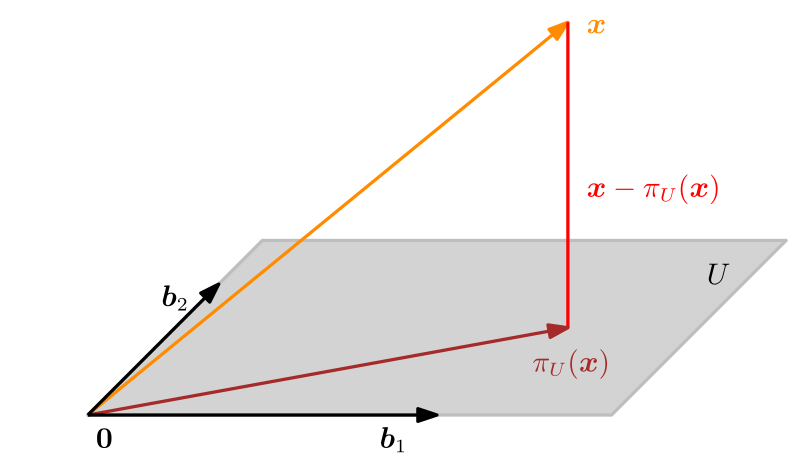
\includegraphics[width=10cm]{9}\\
\centering
\textbf{Figure}: Projection onto a two-dimensional subspace $U$ with basis $\bm{b}_1$ and $\bm{b}_2$
\end{figure}\\
Assume that $(\bm{b}_1,\ldots,\bm{b}_m)$ is an ordered basis of $U$. Any projection $\pi_U(\bm{x})$ onto $U$ is 
an element of $U$; therefore they can be represented
as linear combinations of the basis vectors $\bm{b}_1,\ldots,\bm{b}_m$ of $U$, such that
$\pi_U(\bm{x})=\sum^m_{i=1}\lambda_i\bm{b}_i$.\\
\vspace{1mm}\\
\textbf{Deriving the projection}\\
Procedurally similar to the one-dimensional case:
\begin{enumerate}
\item\textbf{Determining coordinates of projection}\\
We want the coordinates $\lambda_1,\ldots,\lambda_m$ of the projection (with respect to the basis of $U$), 
such that the linear combination
\begin{align*}
&\pi_U(\bm{x})=\sum^m_{i=1}\lambda_i\bm{b}_i=\bm{B\lambda}\\
\text{where}\quad&\bm{B}=[\bm{b_1},\ldots,\bm{b_m}]\in\mathbb{R}^{n\times m},\quad\bm{\lambda}
=[\lambda_1,\ldots,\lambda_m]^T\in\mathbb{R}^m
\end{align*}
is closest to $\bm{x}\in\mathbb{R}^n$. Similar to the 1D case, this implies that
the vector connecting $\pi_U(\bm{x})\in U$ and $\bm{x}\in\mathbb{R}^n$ must be orthogonal to all
basis vectors in $U$.\\
(next page)
\newpage
\noindent The vector connecting $\pi_U(\bm{x})\in U$ and $\bm{x}\in\mathbb{R}^n$ must be orthogonal to all
basis vectors in $U$---so we have $m$ simultaneous conditions. Assuming the dot product as the inner product:
\begin{align*}
\langle\bm{b}_1,\bm{x}-\pi_U(\bm{x})\rangle&=
\bm{b}_1^T(\bm{x}-\pi_U(\bm{x}))=0\\
&\vdots\\
\langle\bm{b}_m,\bm{x}-\pi_U(\bm{x})\rangle&=
\bm{b}_m^T(\bm{x}-\pi_U(\bm{x}))=0
\end{align*}
since $\pi_U(\bm{x})=\bm{B\lambda}$, we have
\begin{align*}
\bm{b}_1^T(\bm{x}&-\bm{B\lambda})=0\\
&\vdots\\
\bm{b}_m^T(\bm{x}&-\bm{B\lambda})=0
\end{align*}
This can be written compactly as
\begin{align*}
\underbrace{\begin{bmatrix}
\bm{b}_1^T\\\vdots\\\bm{b}_m^T
\end{bmatrix}}_{m\times n}
\underbrace{\begin{bmatrix}
\bm{x}-\bm{B\lambda}
\end{bmatrix}}_{n\times1}&=\bm{0}
\iff\bm{B}^T(\bm{x}-\bm{B\lambda})=\bm{0}\\
&\iff\bm{B}^T\bm{B\lambda}=\bm{B}^T\bm{x}
\end{align*}
This expression is called the \textit{normal equation}. Since $\bm{b}_1,\ldots,\bm{b}_m$ are a basis 
of $U$ and therefore linearly independent (since rk($\bm{B})=$rk($\bm{B}^T$) meaning $B^TB$ can be seen as 
linear combinations of linearly independent vectors with linearly independent coefficients, making 
the result linearly independent (\ref{fundamentals:ALCOLIVALI})), $B^TB\in\mathbb{R}^{m\times m}$ is full rank
and invertible. So we have
\begin{equation*}
\lambda=(\bm{B}^T\bm{B})^{-1}\bm{B}^T\bm{x}
\end{equation*}
The matrix $\bm{B}^T\bm{B}$ will always be symmetric and positive semidefinite; symmetry is obvious, 
positive definiteness comes from $\bm{x}^T(\bm{B}^T\bm{B})\bm{x}=(\bm{Bx})^T(\bm{Bx})\geq\bm{0}$.
Invertibility of $\bm{B}^T\bm{B}$ comes from $\bm{B}$ being a basis and therefore full rank.\\
\vspace{1mm}\\
The matrix $(\bm{B}^T\bm{B})^{-1}\bm{B}^T$ is also called the \textit{psuedo-inverse} of $\bm{B}$.\\
(next page)
\newpage
\item\textbf{Finding the projection point}\\
We want the projection point $\pi_U(\bm{x})$; since $\pi_U(\bm{x})=\bm{B\lambda}$, we have
\begin{equation*}
\pi_U(\bm{x})=\bm{B\lambda}=\bm{B}(\bm{B}^T\bm{B})^{-1}\bm{B}^T\bm{x}
\end{equation*}
\item\textbf{Finding the projection matrix}
We can immediately see that the projection matrix that solves $\bm{P}_\pi\bm{x}=\pi_U(\bm{x})$ would be
\begin{equation*}
\bm{P}_\pi=\bm{B}(\bm{B}^T\bm{B})^{-1}\bm{B}^T
\end{equation*}
Notice that this general expression includes the 1D case as a special case, where if dim($U)=1$, 
then $\bm{B}^T\bm{B}\in\mathbb{R}$ is a scalar so $\bm{P}_\pi=\bm{B}(\bm{B}^T\bm{B})^{-1}\bm{B}^T
=\frac{\bm{B}\bm{B}^T}{\bm{B}^T\bm{B}}$ (which is the projection matrix in the 1D case).
\end{enumerate}
\textbf{Example}: 2D case\\
Considering a subspace $U=\text{span}[
\begin{bmatrix}1\\1\\1\end{bmatrix},
\begin{bmatrix}0\\1\\2\end{bmatrix}]\subseteq
\mathbb{R}^3$ and $\bm{x}=
\begin{bmatrix}6\\0\\0\end{bmatrix}\in\mathbb{R}^3$, we 
want the coordinates $\bm{\lambda}$ of the projection of $\bm{x}$ onto $U$, the projection point $\pi_U(\bm{x})$,
and the projection matrix $\bm{P}_\pi$.\\
\vspace{1mm}\\
First we see that the generating set of $U$ is a basis (linear independence) and write the basis of $U$ as a
matrix $\bm{B}=\begin{bmatrix}1&0\\1&1\\1&2\end{bmatrix}$. Next we compute the 
matrix $\bm{B}^T\bm{B}$ and the vector $\bm{B}^T\bm{x}$: 
\begin{equation*}
\bm{B}^T\bm{B}=\begin{bmatrix}1&1&1\\0&1&2\end{bmatrix}
\begin{bmatrix}1&0\\1&1\\1&2\end{bmatrix}
=\begin{bmatrix}3&3\\3&5\end{bmatrix},\quad
\bm{B}^T\bm{x}=\begin{bmatrix}1&1&1\\0&1&2\end{bmatrix}
\begin{bmatrix}6\\0\\0\end{bmatrix}=
\begin{bmatrix}6\\0\end{bmatrix}
\end{equation*}
we solve the normal equation $\bm{B}^T\bm{B\lambda}=\bm{B}^T\bm{x}$ to find $\bm{\lambda}$:
\begin{equation*}
\begin{bmatrix}3&3\\3&5\end{bmatrix}
\begin{bmatrix}\lambda_1\\\lambda_2\end{bmatrix}
=\begin{bmatrix}6\\0\end{bmatrix}\iff
\bm{\lambda}=\begin{bmatrix}
5\\-3\end{bmatrix}
\end{equation*}
The projection point $\pi_U(\bm{x})$ can be directly computed since $\pi_U(\bm{x})=\bm{B\lambda}$:
\begin{equation*}
\pi_U(\bm{x})=\bm{B\lambda}=\begin{bmatrix}
5\\2\\-1\end{bmatrix}
\end{equation*}
The projection matrix (for any $\bm{x}\in\mathbb{R}^3$) is given by
\begin{equation*}
\bm{P}_\pi=\bm{B}(\bm{B}^T\bm{B})^{-1}\bm{B}^T=\frac{1}{6}
\begin{bmatrix}
5&2&-1\\2&2&2\\-1&2&5
\end{bmatrix}
\end{equation*}
(next page)
\newpage
\noindent\textbf{Remarks}\\
The projections $\pi_U(\bm{x})$ are still vectors in $\mathbb{R}^n$---they just lie in an $m$-dimensional 
subspace $U\subseteq\mathbb{R}^n$. To represent
a projected point we only need $m$ coordinates $\lambda_1,\ldots,\lambda_m$ with 
respect to the basis vectors $\bm{b}_1,\ldots,\bm{b}_m$ of $U$.\\
\vspace{1mm}\\
In vector spaces with general inner products, we have to pay attention when computing angles
and distances, which are defined by means of the inner product.\\
\vspace{1mm}\\
\textbf{Utility of Projections in unsolvable linear systems}\\
Projections are useful in situations where we have a linear system $\bm{Ax}=\bm{b}$ without a solution, 
meaning $\bm{b}$ does not lie in the span of $\bm{A}$ (the column space of $\bm{A}$). 
Since we cannot find an exact solution we can find an \textit{approximate solution} by finding the vector in
the column space of $\bm{A}$ that is closest to $\bm{b}$---computing the orthogonal projection of 
$\bm{b}$ onto the column space of $\bm{A}$. (this solution is called the \textit{least-squares solution} 
when the dot product is used as the inner product)\\
\vspace{1mm}\\
\textbf{Utility of an Orthonormal Basis in finding projections}\\
Should the subspace $U$ that we are projecting onto have an orthonormal basis, notice that since 
$\bm{B}^T\bm{B}=\bm{I}$ the projection equation simplifies greatly to
\begin{equation*}
\pi_U(\bm{x})=\bm{BB}^T\bm{x}
\end{equation*}
we no longer have to compute $(\bm{B}^T\bm{B})^{-1}$, which saves computation time.
\newpage

\subsection{Gram-Schmidt Orthogonalisation}%290724
The Gram-Schmidt method uses projections to constructively transform any basis 
$(\bm{b}_1,\ldots,\bm{b}_n)$ of an $n$-dimensional vector space $V$ into an orthogononal or orthonormal basis 
$(\bm{u}_1,\ldots,\bm{u}_n)$ of $V$. An orthogonal basis is iteratively constructed from any basis as follows:
\begin{align*}
\bm{u}_1&:=\bm{b}_1\\
\bm{u}_k&:=\bm{b}_k-\pi_{\text{span}[\bm{u}_1,\ldots,\bm{u}_{k-1}]}(\bm{b}_k),\quad
k=2,\ldots,n
\end{align*}
The $k$th basis vector $\bm{b}_k$ is projected onto the subspace spanned by the first $k-1$ constructed
orthogonal vectors $\bm{u}_1,\ldots,\bm{u}_{k-1}$. This
projection is then subtracted from $\bm{b}_k$ and yields
a vector $\bm{u}_k$ that is orthogonal to the 
$(k-1)$-dimensional subspace spanned by $\bm{u}_1,\ldots,\bm{u}_{k-1}$.
\begin{figure}[h]
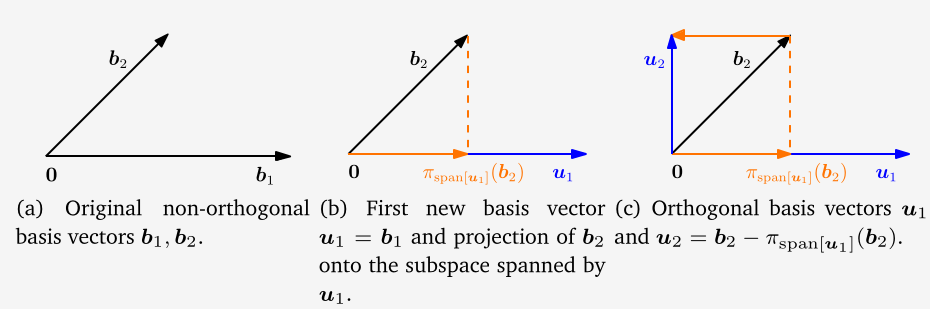
\includegraphics[width=10cm]{10}\\
\centering
\end{figure}\\
Repeating this procedure for all $n$ original basis vectors $(\bm{b}_1,\ldots,\bm{b}_n)$ 
yields an orthogonal basis $(\bm{u}_1,\ldots,\bm{u}_n)$ of $V$.
If we normalise the $\bm{u}_k$ we then obtain an orthonormal basis where $||\bm{u}_k||=1$ for all $k=1,\ldots,n$.\\
\vspace{1mm}\\
\textbf{Example}\\
Consider a basis $(\bm{b}_1,\bm{b}_2)$ of $\mathbb{R}^2$, where
\begin{equation*}
\bm{b}_1=\begin{bmatrix}2\\0\end{bmatrix},\quad
\bm{b}_2=\begin{bmatrix}1\\1\end{bmatrix}
\end{equation*}
Using the Gram-Schmidt method we construct an orthogonal basis $(\bm{u}_1,\bm{u}_2)$ of $\mathbb{R}^2$ as follows
(assuming the dot product as the inner product):
\begin{align*}
\bm{u}_1&=\bm{b}_1\\
\bm{u}_2&=\bm{b}_2-\pi_{\text{span}[\bm{u}_1]}(\bm{b}_2)
=\bm{b}_2-\frac{\bm{u}_1\bm{u}_1^T}{||\bm{u}_1||^2}\bm{b}_2=\begin{bmatrix}1\\1\end{bmatrix}
-\begin{bmatrix}1&0\\0&0\end{bmatrix}
\begin{bmatrix}1\\1\end{bmatrix}
=\begin{bmatrix}0\\1\end{bmatrix}
\end{align*}
see that $\bm{u}_1$ and $\bm{u}_2$ are orthogonal: $\bm{u}_1^T\bm{u}_2=0$
\newpage

\subsection{Projection onto Affine Subspaces} %300724
Given an affine space $L=\bm{x}_0+U$, where $\bm{b}_1,\bm{b}_2$ are basis vectors of $U$, we want 
to determine the orthogonal projection $\pi_L(\bm{x})$ of some $\bm{x}$ onto $L$.
\begin{figure}[h]
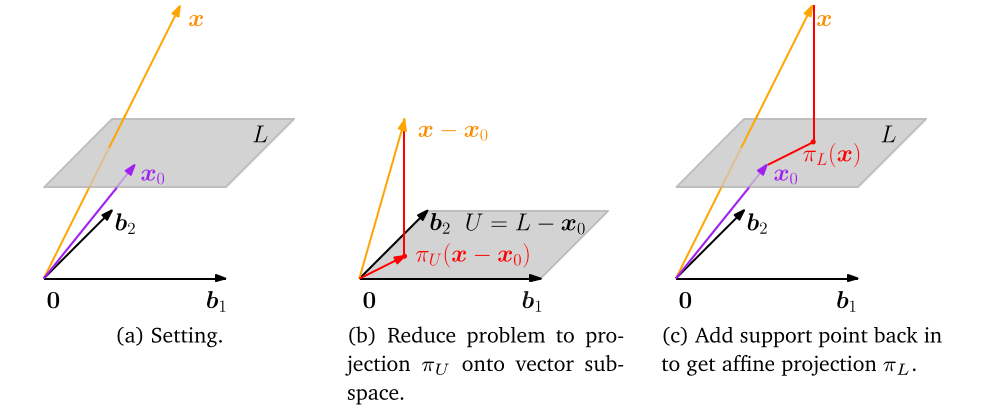
\includegraphics[width=10cm]{11}\\
\centering
\end{figure}\\
An approach would be to subtract the support point $\bm{x}_0$ from $\bm{x}$ and from $L$, since $L-\bm{x}_0=U$.
We then take the projection $\pi_U(\bm{x}-\bm{x}_0)$, then translate the projection back to $L$ 
by adding $\bm{x}_0$:
\begin{equation*}
\pi_L(\bm{x})=\bm{x}_0+\pi_U(\bm{x}-\bm{x}_0)
\end{equation*}
Notice that the distance of $\bm{x}$ from the affine space $L$ is equal to the distance of $\bm{x}-\bm{x}_0$
from $U$:
\begin{align*}
d(\bm{x},L)&=||\bm{x}-\pi_L(\bm{x})||=||\bm{x}-(\bm{x}_0
+\pi_U(\bm{x}-\bm{x}_0))||\\
&=d(\bm{x}-\bm{x}_0,\pi_U(\bm{x}-\bm{x}_0))
=d(\bm{x}-\bm{x}_0,U)
\end{align*}
\newpage

\subsection{Rotations} %300724
Orthogonal transformation matrices (\ref{analytic geometry:orthogonal matrices}) preserve length and angle; 
some of these matrices describe rotations.\\
\vspace{1mm}\\
\textbf{Rotations in $\mathbb{R}^2$}\\
A \textit{rotation} is a linear mapping (an automorphism) that rotates a plane by an angle $\theta$ about the
origin. Considering the standard basis $\left\{\bm{e}_1=
\begin{bmatrix}1\\0\end{bmatrix},\bm{e}_2=\begin{bmatrix}
0\\1\end{bmatrix}\right\}$,
say we want to rotate this coordinate system by an angle 
$\theta$:
\begin{figure}[h]
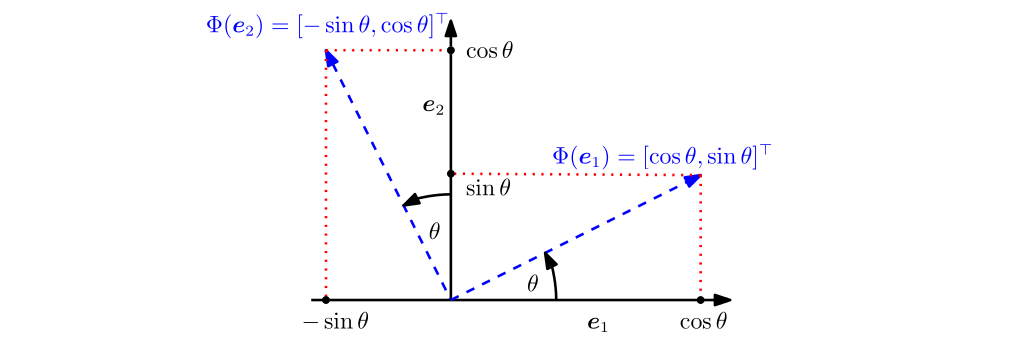
\includegraphics[width=10cm]{12}\\
\centering
\end{figure}\\
Rotations $\Phi$ are linear mappings so we can express them by a \textit{rotation matrix} $\bm{R}(\theta)$. 
We determine the coordinates of the rotated axes (the image of $\Phi$) with respect to the standard
basis:
\begin{equation*}
\Phi(\bm{e}_1)=\begin{bmatrix}\cos\theta\\\sin\theta\end{bmatrix},\quad
\Phi(\bm{e}_2)=\begin{bmatrix}-\sin\theta\\\cos\theta\end{bmatrix}
\end{equation*}
Therefore the rotation that performs the basis change into the rotated coordinates $\bm{R}(\theta)$ is given as
\begin{equation*}
\bm{R}(\theta)=\begin{bmatrix}\Phi(\bm{e}_1)&\Phi(\bm{e}_2)\end{bmatrix}
=\begin{bmatrix}\cos\theta&-\sin\theta\\\sin\theta&\cos\theta\end{bmatrix}
\end{equation*}
(next page)
\newpage
\noindent\textbf{Rotations in $\mathbb{R}^3$}\\
In contrast to the $\mathbb{R}^2$ case, in $\mathbb{R}^3$ we can rotate any two-dimensional plane about a
one-dimensional axis. The easiest way to specify the general rotation matrix is to specify the images of the 
standard basis, and making sure they are orthonormal to each other (so we get an orthogonal matrix which
preserves length and angle).\\
\vspace{1mm}\\
We define a `counterclockwise' rotation about an axis as
a rotation about that axis when we look
at it `head on, from the end toward the origin'. Therefore in $\mathbb{R}^3$ there are three (planar) 
rotations about the three standard basis vectors:
\begin{itemize}
\item Rotation about the $\bm{e}_3$-axis:
\begin{equation*}
\bm{R}_3(\theta)=\begin{bmatrix}\Phi(\bm{e}_1)&\Phi(\bm{e}_2)&\Phi(\bm{e}_3)\end{bmatrix}=
\begin{bmatrix}\cos\theta&-\sin\theta&0\\
\sin\theta&\cos\theta&0\\0&0&1\end{bmatrix}
\end{equation*}
The $\bm{e}_3$ coordinate is fixed (its image is therefore the same), and counterclockwise rotation is
performed in the $\bm{e}_1\bm{e}_2$ plane. We look at $\bm{e}_3$ from its `tip' toward the origin:
\begin{figure}[h]
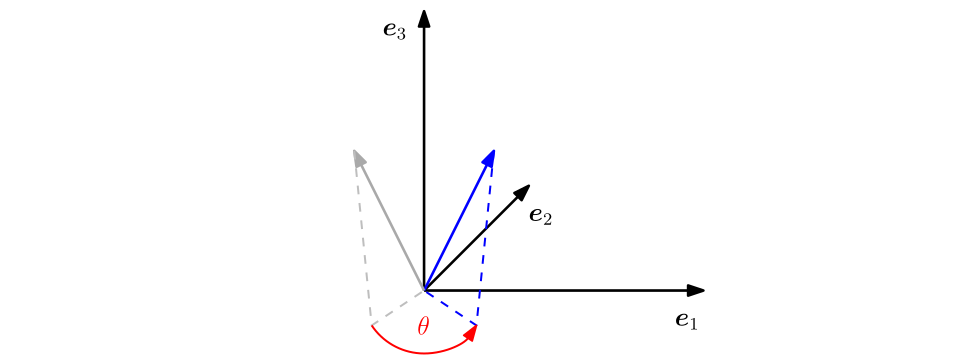
\includegraphics[width=10cm]{13}\\
\centering
\end{figure}
\item Rotation about the $\bm{e}_1$-axis (counterclockwise):
\begin{equation*}
\bm{R}_1(\theta)=
\begin{bmatrix}1&0&0\\
0&\cos\theta&-\sin\theta\\
0&\sin\theta&\cos\theta\end{bmatrix}
\end{equation*}
\item Rotation about the $\bm{e}_2$-axis (clockwise):
\begin{equation*}
\bm{R}_2(\theta)=
\begin{bmatrix}
\cos\theta&0&\sin\theta\\
0&1&0\\-\sin\theta&0&\cos\theta\end{bmatrix}
\end{equation*}
\end{itemize}
(next page)
\newpage
\noindent\textbf{Rotations in $n$ Dimensions}\\
The generalisation of rotations from 2D to 3D to $n$-dimensional Euclidean vector spaces can be intuitively
described as fixing $n$-2 dimensions and restricting the 
rotation to a two-dimensional plane in the $n$-dimensional space; here we describe the Givens Rotation:\\
\vspace{1mm}\\
\textbf{Givens rotation}\\
Let $V$ be an $n$-dimensional Euclidean vector space and $\Phi:V\to V$ an automorphism with transformation matrix
\begin{equation*}
\bm{R}_{ij}(\theta):=\begin{bmatrix}
\bm{I}_{i-1}&\bm{0}&\cdots&\cdots&\bm{0}\\
\bm{0}&\cos\theta&\bm{0}&-\sin\theta&\bm{0}\\
\bm{0}&\bm{0}&\bm{I}_{j-i-1}&\bm{0}&\bm{0}\\
\bm{0}&\sin\theta&\bm{0}&\cos\theta&\bm{0}\\
\bm{0}&\cdots&\cdots&\bm{0}&\bm{I}_{n-j}
\end{bmatrix}
\end{equation*}
for $1\leq i<j\leq n$ and $\theta\in\mathbb{R}$. Then $\bm{R}_{ij}$ is called a \textit{Givens rotation}.
Essentially, $\bm{R}_{ij}$ is the identity matrix $\bm{I}_n$ with
\begin{equation*}
r_{ii}=\cos\theta,\quad r_{ij}=-\sin\theta,\quad
r_{ji}=\sin\theta,\quad r_{jj}=\cos\theta
\end{equation*}
\textbf{Properties of Rotations}
Most properties of rotations come from them being orthogonal matrices:
\begin{itemize}
\item Rotations preserve distances, meaning $||\bm{x}-\bm{y}||=||\bm{R}_\theta\bm{x}-\bm{R}_\theta\bm{y}||$.
\item Rotations preserve angles, meaning the angle between
$\bm{R}_\theta\bm{x}$ and $\bm{R}_\theta\bm{y}$ equals the angle between $\bm{x}$ and $\bm{y}$.
\item Rotations in three or more dimensions are generally non commutative. 
Only in two dimensions are vector rotations commutative, this means 
$\bm{R}(\phi)\bm{R}(\theta)=\bm{R}(\phi)\bm{R}(\theta)$
for all $\phi,\theta\in[0,2\pi]$. They form an Abelian group (with multiplication) only
if they rotate about the same point.
\end{itemize}
\newpage

\section{Matrix Decompositions} %020824
\subsection{Properties of the determinant}
Geometrically the determinant of a matrix represents the signed volume of the parallelepiped formed
by the columns of that matrix.\\
\vspace{1mm}\\
For $\bm{A}\in\mathbb{R}^{n\times n}$ the determinant exhibits the following properties:
\begin{itemize}
\item The determinant of a matrix product is the product of the corresponding determinants, meaning
$\text{det}(\bm{AB})=\text{det}(\bm{A})\text{det}(\bm{B})$.
\item Determinants are invariant to transposition, meaning
$\text{det}(\bm{A})=\text{det}(\bm{A}^T)$.
\item If $\bm{A}$ is invertible/regular, then $\text{det}(\bm{A}^{-1})=\frac{1}{\text{det}(\bm{A})}$.
\item Similar matrices (\ref{fundamentals:equivalence and similarity}) possess the same determinant.
Therefore for a linear mapping $\Phi:V\to V$ all transformation matrices $\bm{A}_\Phi$ of $\Phi$ have the same
determinant; the determinant is invariant to the choice of basis for a linear mapping.
\item Adding a multiple of a column/row to another one does not change $\text{det}(\bm{A})$.
\item Multiplication of a column/row with $\lambda\in\mathbb{R}$ scales $\text{det}(\bm{A})$
by $\lambda$. In particular, $\det{\lambda\bm{A}}=\lambda^n\text{det}(\bm{A})$.
\item Swapping two columns changes the sign of $\text{det}(\bm{A})$.
\end{itemize}
Notice that because of the last three properties, we can use Gaussian elimination to compute $\text{det}(\bm{A})$
by bringing $\bm{A}$ to row-echelon form. We can stop Gaussian elimination when we have $\bm{A}$
in upper triangular form---so that the determinant 
is just the product of the diagonal elements.\\
\vspace{1mm}\\
\textbf{Determinant and Rank}\\
Theorem: \textit{A square matrix $\bm{A}\in\mathbb{R}^{n\times b}$ has $\text{det}(\bm{A})\neq0$ if and only
if $\text{rk}(\bm{A})=n$. In other words, $\bm{A}$ is invertible if and only if it is full rank.}
\newpage

\subsection{Trace} %020824
The \textit{trace} of a square matrix $\bm{A}^{n\times n}$ is 
defined as 
\begin{equation*}
\text{tr}(A):=\sum^n_{i=1}a_{ii}
\end{equation*}
essentially the sum of the elements on the main diagonal.
\\
\vspace{1mm}\\
The trace satisfies the following properties:
\begin{itemize}
\item tr$(\bm{A+B})=\text{tr}(A)+\text{tr}(\bm{B})$ for
$\bm{A},\bm{B}\in\mathbb{R}^{n\times n}$
\item tr$(\alpha\bm{A})=\alpha\text{tr}(\bm{A}),\,\alpha\in\mathbb{R}$ for $\bm{A}\in\mathbb{R}^{n\times n}$.
\item tr$(\bm{I}_n)=n$
\item tr$(\bm{AB})=\text{tr}(\bm{BA})$ for $\bm{A}\in\mathbb{R}^{n\times k},\bm{B}^{k\times n}$
\end{itemize}
\textbf{Invariance under cyclic permutation}\\
Notice that the last property can be extended---
the trace is invariant under cyclic permutation of matrix products:
\begin{equation*}
\text{tr}(\bm{AKL})=\text{tr}(\bm{KLA})
\end{equation*}
For matrices $\bm{A}\in\mathbb{R}^{n\times k},\bm{K}\in\mathbb{R}^{k\times l},\bm{L}\in\mathbb{R}^{l\times n}$.
This property generalises to products of an arbritrary number of matrices. 
A special case of this should be noted: for two vectors 
$\bm{x},\bm{y}\in\mathbb{R}^n$
\begin{equation*}
\text{tr}(\bm{xy}^T)=\text{tr}(\bm{y}^T\bm{x})=\bm{y}^T\bm{x}\in\mathbb{R}
\end{equation*}
(next page)
\newpage
\noindent\textbf{Trace, Linear mappings, and Basis changes}\\
Given a linear mapping $\Phi:V\to V$, where $V$ is a vector space, we define the trace of this map
by using the trace of the matrix representation of $\Phi$;
for a given basis of $V$, we can describe $\Phi$ by means
of the transformation matrix $\bm{A}$, where the trace of $\Phi$ is the trace of $\bm{A}$.\\
\vspace{1mm}\\
For a different basis of $V$, it holds that the corresponding transformation matrix $\bm{B}$ of $\Phi$ can be
obtained by a basis change of the form $\bm{S}^{-1}\bm{AS}$ for suitable $\bm{S}$ (\ref{fundamentals:basis change}).
For the corresponding trace of $\Phi$, this means
\begin{equation*}
\text{tr}(\bm{B})=\text{tr}(\bm{S}^{-1}\bm{AS})=
\text{tr}(\bm{AS}\bm{S}^{-1})=\text{tr}(\bm{A})
\end{equation*}
While matrix representations of linear mappings are basis dependent, the trace of a linear mapping $\Phi$ 
is independent of the basis.
\newpage

\subsection{Eigenvalues, Eigenvectors, Characteristic Polynomial}%020824
\textbf{Definition of Characteristic polynomial}\\
For $\lambda\in\mathbb{R}$ and a square matrix $A\in\mathbb{R}^{n\times n}$
\begin{align*}
p_{\bm{A}}(\lambda)&:=\text{det}(\bm{A}-\lambda\bm{I})\\
&=c_0+c_1\lambda+c_2\lambda^2+\ldots+c_{n-1}\lambda^{n-1}
+(-1)^n\lambda^n
\end{align*}
$c_0,\ldots,c_{n-1}\in\mathbb{R}$ is the characteristic polynomial of $\bm{A}$. In particular,
\begin{align*}
c_0&=\text{det}(\bm{A})\\
c_{n-1}&=(-1)^{n-1}\text{tr}(\bm{A})
\end{align*}
Motivation for the characteristic polynomial comes from its utility in computing eigenvalues and eigenvectors.\\
\vspace{1mm}\\
\textbf{Eigenvectors and Eigenvalues}\\
\textbf{Definition}: Let $\bm{A}\in\mathbb{R}^{n\times n}$ be a square matrix. Then $\lambda\in\mathbb{R}$ is an \textit{eigenvalue} of $\bm{A}$ and $\bm{x}\in\mathbb{R}^n
\backslash\{\bm{0}\}$ is the corresponding \textit{eigenvector} of $\bm{A}$ if
\begin{equation*}
\bm{Ax}=\bm{\lambda x}
\end{equation*}
the above is called the \textit{eigenvalue equation}. The following statements are equivalent:
\begin{itemize}
\item$\lambda$ is an eigenvalue of $\bm{A}\in\mathbb{R}^{n\times n}$.
\item There exists an $\bm{x}\in\mathbb{R}^n\backslash\{\bm{0}\}$ with $\bm{Ax}=\bm{\lambda x}$; or equivalently,
$(\bm{A}-\lambda\bm{I}_n)\bm{x}=\bm{0}$ can be solved non trivially. 
(If an eigenvalue exists then an eigenvector exists.)
\item rk$(\bm{A}-\lambda\bm{I}_n)<n$ (since there are nontrivial solutions).
\item det$(\bm{A}-\lambda\bm{I}_n)=0$
\end{itemize}
Notice this motivates the necessity for the characteristic equation---
$\lambda\in\mathbb{R}$ is an eigenvalue of $\bm{A}\in\mathbb{R}^{n\times n}$ if and only if $\lambda$ is a root
of the characteristic polynomial $p_{\bm{A}}(\lambda)$ of $\bm{A}$.\\
\vspace{1mm}\\
\textbf{Collinearity, Codirection---definition and significance}\\
Two vectors that point in the same direction are called \textit{codirected}. Two vectors are \textit{collinear} if
they point in the same or opposite direction.\\
\vspace{1mm}\\
If $\bm{x}$ is an eigenvector of $\bm{A}$ associated with eigenvalue $\lambda$, then for any 
$c\in\mathbb{R}\backslash\{\bm{0}\}$ it holds that $c\bm{x}$ is an eigenvector of 
$\bm{A}$ with the same eigenvalue since
\begin{equation*}
\bm{A}(c\bm{x})=c\bm{A}(\bm{x})=c\lambda(\bm{x})
=\lambda(c\bm{x})
\end{equation*}
All vectors that are collinear to $\bm{x}$ are also eigenvectors of $\bm{A}$.\\
(next page)
\newpage
\noindent\textbf{Algebraic multiplicity}\\
Let a square matrix $\bm{A}$ have an eigenvalue $\lambda$. The \textit{algebraic multiplicity} of $\lambda$ is
the number of times the root appears in the characteristic polynomial.\\
\vspace{1mm}\\
\textbf{Eigenspace and Eigenspectrum}\\
For $\bm{A}\in\mathbb{R}^{n\times n}$ the set of all eigenvectors of $\bm{A}$ associated with eigenvalue 
$\lambda$ spans a subspace of $\mathbb{R}^n$ called the \textit{eigenspace} of $\bm{A}$ with respect to 
$\lambda$ and is denoted by $E_\lambda$. The set of eigenvalues of $\bm{A}$ is called the 
\textit{eigenspectrum/spectrum} of $\bm{A}$.\\
\vspace{1mm}\\
If $\lambda$ is an eigenvalue of $\bm{A}\in\mathbb{R}^{n\times n}$, then the corresponding eigenspace is the 
solution space of $(\bm{A}-\lambda\bm{I})\bm{x}=\bm{0}$. 
\\
\vspace{1mm}\\
\textbf{Notable properties}
\begin{itemize}
\item A matrix $\bm{A}$ and its transpose $\bm{A}^T$ possess the same eigenvalues, but not necessarily the
same eigenvectors (for intuition, recall that the determinant is invariant with respect to transposition)
\item The eigenspace $E_\lambda$ is the nullspace of 
$\bm{A}-\lambda\bm{I}$ since
\begin{align*}
\bm{Ax}=\lambda\bm{x}&\iff\bm{Ax}-\lambda\bm{x}=\bm{0}\\
&\iff(\bm{A}-\lambda\bm{I})\bm{x}=\bm{0}\iff\bm{x}
\in\text{ker}(\bm{A}-\lambda\bm{I})
\end{align*}
\item Similar matrices possess the same eigenvalues. Therefore a linear mapping $\Phi$ has eigenvalues that are
independent of the choice of basis of its transformation matrix. 
(this makes eigenvalues, together with the determinant and the trace, key characteristic parameters of a linear
mapping as they are all invariant under basis change)
\item Symmetric, positive definite matrices always have positive, real eigenvalues (\ref{matrix dec:smahre}).
\end{itemize}
\textbf{The case of the identity matrix}\\
The identity matrix $\bm{I}\in\mathbb{R}^{n\times n}$ has characteristic polynomial $p_I(\lambda)=\text(det)
(\bm{I}-\lambda\bm{I})=(1-\lambda)^n=0$, which only has one eigenvalue $\lambda=1$ that occurs $n$ times.\\
\vspace{1mm}\\
Moreover, $\bm{Ix}=\lambda\bm{x}=1\bm{x}$ holds for all vector
$\bm{x}\in\mathbb{R}\backslash\{\bm{0}\}$; because of this the sole eigenspace $E_1$ of the identity matrix
spans $n$ dimensions, and all $n$ standard basis vectors
of $\mathbb{R}^n$ are eigenvectors of $\bm{I}$.\\
(next page)
\newpage
\noindent\textbf{Example}: Computing Eigenvectors, Eigenvalues, and Eigenspaces\\
Consider finding the eigenvalues and eigenvectors of the 2 $\times$ 2 matrix
\begin{equation*}
\bm{A}=\begin{bmatrix}
4&2\\1&3\end{bmatrix}
\end{equation*}
\textbf{Step 1: Characteristic polynomial}\\
The necessity for the characteristic polynomial comes from the idea 
that there will be a vector such that $\bm{Ax}=\lambda\bm{x}$, meaning $(\bm{A}-\lambda\bm{I})\bm{x}=\bm{0}$. For
$\bm{x}\neq\bm{0}$ this requires that the kernel of 
$\bm{A}-\lambda\bm{I}$ contains more than just $\bm{0}$;
this means that $\bm{A}-\lambda\bm{I}$ is not invertible and therefore that $\text{det}(\bm{A}-\lambda\bm{I})=0$.
Hence we need to compute the roots of the characteristic 0polynomial to find the eigenvalues. This is given by
\begin{align*}
p_{\bm{A}}(\lambda)&=\text{det}(\bm{A}-\lambda\bm{I})\\
&=\text{det}\left(\begin{bmatrix}
4&2\\1&3\end{bmatrix}-
\begin{bmatrix}\lambda&0\\0&\lambda\end{bmatrix}\right)
=\begin{vmatrix}4-\lambda&2\\1&3-\lambda\end{vmatrix}\\
&=(4-\lambda)(3-\lambda)-2\cdot1
\end{align*}
Factorising, we obtain
\begin{equation*}
p_{\bm{A}}(\lambda)=(2-\lambda)(5-\lambda)
\end{equation*}
with that we have the eigenvalues $\lambda_1=2$ and $\lambda_2=5$.\\
\vspace{1mm}\\
\textbf{Step 2: Eigenvectors and Eigenspaces}\\
We find the eigenvectors by solving for $\bm{x}$ in the aforementioned system:
\begin{equation*}
\begin{bmatrix}4-\lambda&2\\1&3-\lambda\end{bmatrix}\bm{x}=\bm{0}
\end{equation*}
For $\lambda=5$ we obtain
\begin{equation*}
\begin{bmatrix}4-5&2\\1&3-5\end{bmatrix}
\begin{bmatrix}x_1\\x_2\end{bmatrix}
=\begin{bmatrix}-1&2\\1&-2\end{bmatrix}\begin{bmatrix}x_1\\x_2\end{bmatrix}
=\bm{0}
\end{equation*}
Solving this homogeneous system we obtain a solution space
\begin{equation*}
E_5=\text{span}[\begin{bmatrix}2\\1\end{bmatrix}]
\end{equation*}
This eigenspace is one dimensional since it contains a single basis vector. We analagously solve for 
the eigenvector of $\lambda=2$ to get the eigenspace
\begin{equation*}
E_2=\text{span}[\begin{bmatrix}1\\-1\end{bmatrix}]
\end{equation*}
The two eigenspaces $E_5$ and $E_2$ in this case are one-dimensional as they are each spanned by a single vector. 
However in other cases we may have multiple identical eigenvalues and the eigenspace may have more than one 
dimension.
\newpage

\subsection{Symmetric matrices always have real eigenvalues} %050824
\label{matrix dec:smahre}
Let $(\lambda,\bm{v})$ be any eigenpair of $\bm{A}$. For a symmetric matrix, $\bm{A}=\bm{A}^T$; so
(for the dot product)
\begin{equation*}
\langle\bm{Av},\bm{Av}\rangle=(\bm{Av})^T\bm{Av}
=(\lambda\bm{v})^T\lambda\bm{v}=\lambda^2||\bm{v}||^2
\end{equation*}
Since
\begin{equation*}
\lambda^2=\frac{\langle\bm{Av},\bm{Av}\rangle}{||\bm{v}||^2}
\end{equation*}
is a real nonnegative number, $\lambda$ must be real.
\newpage

\subsection{Eigenvalues and Eigenvectors II} %050824
\textbf{Geometric Multiplicity}\\
Let $\lambda_i$ be an eigenvalue of a square matrix $\bm{A}$. Then the \textit{geometric multiplicity} of
$\lambda_i$ is the number of linearly independent eigenvectors associated with $\lambda_i$---the dimensionality of 
the eigenspace spanned by the eigenvectors associated
with $\lambda_i$.\\
\vspace{1mm}\\
A specific eigenvalue's geometric multiplicity must be at lease one because every eigenvalue has at least one
associated eigenvector. An eigenvalue's geometric multiplicity cannot exceed its algebraic multiplicity, but it may
be lower.\\
\vspace{1mm}\\
\textbf{Graphical intuition in two dimensions}\\
Geometrically, the eigenvector corresponding to a nonzero eigenvalue points in a direction that 
is stretched by the linear mapping. The eigenvalue is a factor by which it is stretched. 
For intuition we present a few examples:
\begin{itemize}
\item $\bm{A}_1=\begin{bmatrix}1/2&0\\0&2\end{bmatrix}$:
\begin{figure}[h]
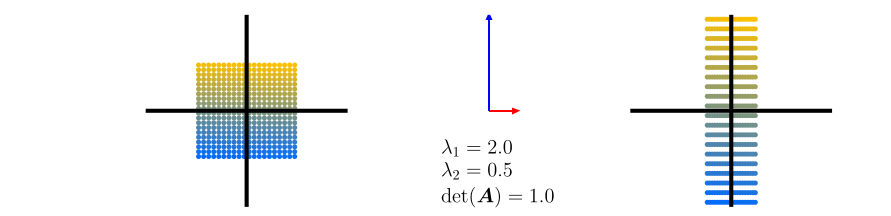
\includegraphics[width=10cm]{14}\\
\centering
\end{figure}\\
The direction of the two eigenvectors correspond to the canonical basis vectors in $\mathbb{R}^2$. The vertical
axis is extended by a factor of 2 (eigenvalue $\lambda_1=2$), and the horizontal axis is compressed by a factor 
of $1/2$ (eigenvalue $\lambda_2=1/2$). The result is area preserving (since det$(\bm{A}_1)=1=2\cdot1/2$).\\
(next page)
\newpage
\item $\bm{A}_2=\begin{bmatrix}1&1/2\\0&1\end{bmatrix}$ 
corresponds to a shear mapping (it shears the points along the horizontal axis to the right
if they are on the positive half of the vertical axis and to the left vice versa):
\begin{figure}[h]

\includegraphics[width=10cm]{15}\\
\centering
\end{figure}\\
This mapping is also area preserving (notice the determinant). The eigenvalue $\lambda_1=1=\lambda_2$ is repeated
and the eigenvectors are collinear. This indicates that the mapping only acts along one direction 
(in this case the horizontal axis).
\item$\bm{A}_3=\begin{bmatrix}
\cos(\pi/6)&-\sin(\pi/6)\\\sin(\pi/6)&\cos(\pi/6)
\end{bmatrix}=\frac{1}{2}\begin{bmatrix}
\sqrt{3}&-1\\1&\sqrt{3}\end{bmatrix}$
\begin{figure}[h]
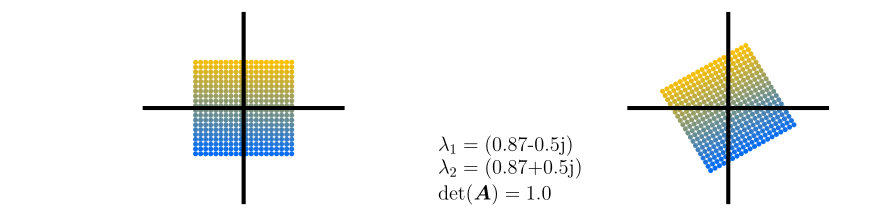
\includegraphics[width=10cm]{16}\\
\centering
\end{figure}\\
This matrix rotates the points by $\frac{\pi}{6}$rad$=30^\circ$ counter-clockwise and has
only complex eigenvalues; this reflects the fact that the matrix represents a rotation mapping (and therefore
doesn't have eigenvectors). Since a rotation is volume preserving, the determinant is 1.\\
(next page)
\newpage
\item$\bm{A_1}=\begin{bmatrix}1&-1\\-1&1\end{bmatrix}$
\begin{figure}[h]
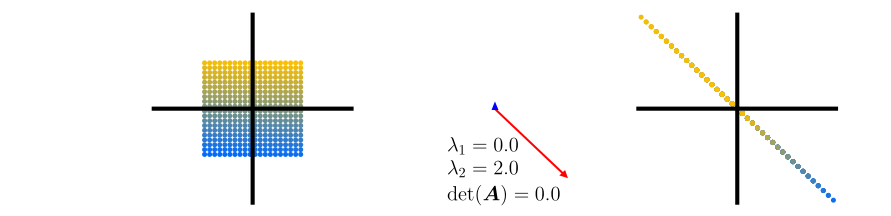
\includegraphics[width=10cm]{17}\\
\centering
\end{figure}\\
represents a mapping that collapses a two-dimensional domain onto one domain. Since one eigenvalue is 0, the space
in the direction of the corresponding eigenvector collapses, while the orthgonal eigenvector stretches space
by a factor $\lambda=2$; therefore the area of the image is 0. (notice the determinant is 0)
\item$\bm{A}_5=\begin{bmatrix}1&1/2\\1/2&1\end{bmatrix}$
\begin{figure}[h]

\includegraphics[width=10cm]{18}\\
\centering
\end{figure}\\
is a stretch-and-shear mapping that scales space by $75\%$
(since $|\text{det}(\bm{A}_5)|=\frac{3}{4}$) it stretches space along the eigenvector of $\lambda=2$ by factor 1.5
and compresses it along the orthogonal eigenvector by factor 0.5.
\end{itemize}
\newpage

\subsection{Eigenvalues and Eigenvectors III} %050824
\textbf{Linear independence of eigenvectors}\\
Theorem: \textit{The eigenvectors $x_1,\ldots,x_n$ of a
matrix $\bm{A}\in\mathbb{R}^{n\times n}$ with $n$ distinct eigenvalues $\lambda_1,\ldots,\lambda_n$ are 
linearly independent.}\\
\vspace{1mm}\\
In essence, the eigenvectors of a matrix with $n$ distinct eigenvalues form a basis of $\mathbb{R}^n$.\\
\vspace{1mm}\\
\textbf{Defective matrices}\\
A square matrix $\bm{A}\in\mathbb{R}^{n\times n}$ is \textit{defective} if it possesses fewer than $n$
linearly independent eigenvectors.\\
\vspace{1mm}\\
A non-defective matrix $\bm{A}\in\mathbb{R}^{n\times n}$ does not necessarily require $n$ distinct eigenvalues,
but rather that the eigenvectors form a basis of $\mathbb{R}^n$. Looking at the eigenvectors of a defective
matrix, it follows that the sum of the dimensions of the eigenspaces is less than $n$.\\
\vspace{1mm}\\
Specifically, a defective matrix has at least one eigenvalue $\lambda_i$, with an algebraic multiplicity $m>1$ but a
geometric multiplicity less than $m$.
This must be the case since a defective matrix cannot have $n$ distinct eigenvalues, 
as distinct eigenvalues have distinct eigenvectors (as per the theorem regarding linear independence of
eigenvectors).
\newpage

\subsection{Symmetry and Positive definiteness of $\bm{A}^T\bm{A}$,\\Spectral Theorem} %060824
\textbf{Symmetry and Positive definiteness of $\bm{A}^T\bm{A}$}\\
Theorem: \textit{Given a matrix $\bm{A}\in\mathbb{R}^{m\times n}$, we can always obtain a symmetric,
positive semidefinite matrix $\bm{S}\in\mathbb{R}^{n\times n}$ by defining}
\begin{equation*}
\bm{S}:=\bm{A}^T\bm{A}
\end{equation*}
See that symmetry comes from 
\begin{equation*}
\bm{S}=\bm{A}^T\bm{A}=\bm{A}^T(\bm{A}^T)^T=(\bm{A}^T\bm{A})^T=\bm{S}^T
\end{equation*}
(recall $(\bm{AB})^T=\bm{B}^T\bm{A}^T$)
(or notice that the element in position $ij$ of the product will always be the same 
as the element in $ji$).\\
\vspace{1mm}\\
Positive definiteness comes from 
\begin{equation*}
\bm{x}^T\bm{Sx}=
\bm{x}^T\bm{A}^T\bm{Ax}=(\bm{x}^T\bm{A}^T)(\bm{Ax})=(\bm{Ax}^T)(\bm{Ax})\geq0
\end{equation*}
because the dot product computes a sum of squares which are non-negative.\\
(next page)
\newpage
\noindent\textbf{Spectral Theorem}\\
\textit{If $\bm{A}\in\mathbb{R}^{n\times n}$ is symmetric, there exists an orthonormal basis of the corresponding 
vector space $V$ consisting of eigenvectors of $\bm{A}$, and each eigenvalue is real.}\\
\vspace{1mm}\\
\textbf{Example}\\
Consider the matrix
\begin{equation*}
\bm{A}=\begin{bmatrix}3&2&2\\2&3&2\\2&2&3\end{bmatrix}
\end{equation*}
The characteristic polynomial of $\bm{A}$ is
\begin{equation*}
p_{\bm{A}}(\lambda)=-(\lambda-1)^2(\lambda-7)
\end{equation*}
so we obtain eigenvalues $\lambda_1=1$ and $\lambda_2=7$, where $\lambda_1$ is a repeat eigenvalue. 
Following the standard procedure for obtaining eigenvectors, we get the eigenspaces
\begin{equation*}
E_1=\text{span}[\underbrace{\begin{bmatrix}-1\\1\\0\end{bmatrix}}_{=:\bm{x}_1},
\underbrace{\begin{bmatrix}-1\\0\\1\end{bmatrix}}_{=:\bm{x}_2}],\quad
E_7=\text{span}[\underbrace{\begin{bmatrix}1\\1\\1\end{bmatrix}}_{\bm{x}_3}]
\end{equation*}
Of the eigenvectors we found, $\bm{x}_3$ is orthogonal to both $\bm{x}_1$ and $\bm{x}_2$, but $\bm{x}_1$ and 
$\bm{x}_2$ are not orthogonal to each other. The spectral
theorem states that there exists an orthogonal basis---we can construct one.\\
\vspace{1mm}\\
To construct such a basis we can exploit the fact that $\bm{x}_1$ and $\bm{x}_2$ are eigenvectors associated with
the same eigenvalue $\lambda$; it holds for any $\alpha,\beta\in\mathbb{R}$ that
\begin{equation*}
\bm{A}(\alpha\bm{x}_1+\beta\bm{x}_2)=
\bm{A}\bm{x}_1\alpha+\bm{A}\bm{x}_2\beta=
\lambda(\alpha\bm{x}_1+\beta\bm{x}_2)
\end{equation*}
Meaning that any linear combination of $\bm{x}_1$ and $\bm{x}_2$ is also an eigenvector of $\bm{A}$ associated
with $\lambda$. We can use the Gram-Schmidt method, since it uses linear combinations (projections), to 
iteratively construct an orthogonal/orthonormal basis.
Therefore even if $\bm{x}_1$ and $\bm{x}_2$ are not orthogonal, applying the Gram-Schmidt algorithm:
\begin{equation*}
\bm{x}'_1=\begin{bmatrix}-1\\1\\0\end{bmatrix},\quad
\bm{x}'_2=\frac{1}{2}\begin{bmatrix}-1\\-1\\2
\end{bmatrix}
\end{equation*}
which are orthogonal to each other and $\bm{x}_3$.
\newpage

\subsection{Determinant, Trace, and Eigenvalues} %070824
\textbf{Eigenvalues and the Determinant}\\
\textbf{Theorem:} \textit{The determinant of a matrix $\bm{A}\in\mathbb{R}^{n\times n}$ is the product of
its eigenvalues:}
\begin{equation*}
\text{det}(\bm{A})=\prod^n_{i=1}\lambda_i
\end{equation*}
\textit{where $\lambda_i\in\mathbb{C}$ are (possibly repeated) eigenvalues of $\bm{A}$.}\\
\vspace{1mm}\\
For geometric intuition, consider a matrix $\bm{A}\in\mathbb{R}^{2\times 2}$ that possesses two linearly independent
eigenvectors $\bm{x}_1,\bm{x}_2$, assume that $(\bm{x}_1,\bm{x}_2)$ are an ONB of $\mathbb{R}^2$ so that
they are orthogonal and the area of the square they span
is 1:
\begin{figure}[h]
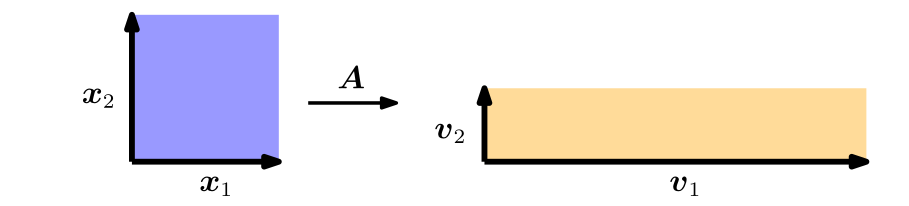
\includegraphics[width=10cm]{19}\\
\centering
\end{figure}\\
We know that the determinant computes the change of the unit square under the transformation $\bm{A}$. 
In this example, we can compute the change of the area explicitly; where 
mapping the eigenvectors using $\bm{A}$ gives us vectors
$\bm{v}_1=\bm{Ax}_1=\lambda\bm{x}_1$ and $\bm{v}_2=\bm{Ax}_2=\lambda\bm{x}_2$---scaled versions of the initial
eigenvectors, scaled by the eigenvalues. Now see that 
the the area of the rectangle that they now span
is the absolute value of the product of the eigenvalues (because $\bm{x}_1$ and $\bm{x}_2$ are orthonormal); the 
area is $|\lambda_1\lambda_2|$. (this is not a rigourous proof by any means, just some intuition)\\
\vspace{1mm}\\
\textbf{Trace and Eigenvalues}\\
\textbf{Theorem:} \textit{The trace of a matrix $\bm{A}\in\mathbb{R}^{n\times n}$ is the sum of its eigenvalues}:
\begin{equation*}
\text{tr}(\bm{A})=\sum^n_{i=1}\lambda_i
\end{equation*}
\textit{where $\lambda_i\in\mathbb{C}$ are (possibly repeated eigenvalues of $\bm{A}$}.\\
\vspace{1mm}\\
This can be proved by comparing coefficients with the equation for the characteristic polynomial.
\newpage

\subsection{Cholesky Decomposition}%080824
With positive real numbers, we have a square-root operation that gives us a decomposition into identical components.
For symmetric, positive definite matrices, the \textit{Cholesky decomposition/factorisation} is one of a number of
operations that provides a square-root equivalent operation that is useful in practice.\\
\vspace{1mm}\\
\textbf{Theorem}: \textit{A symmetric, positive definite matrix $\bm{A}$ can be factorised into a product 
$\bm{A}=\bm{LL}^T$, where $\bm{L}$ is a lower triangular matrix with positive diagonal elements:}
\begin{equation*}
\begin{bmatrix}
a_{11}&\cdots&a_{1n}\\
\vdots&\ddots&\vdots\\
a_{n1}&\cdots&a_{nn}
\end{bmatrix}=
\begin{bmatrix}
l_{11}&\cdots&0\\
\vdots&\ddots&\vdots\\
l_{n1}&\cdots&l_{nn}
\end{bmatrix}
\begin{bmatrix}
l_{11}&\cdots&l_{n1}\\
\vdots&\ddots&\vdots\\
0&\cdots&l_{nn}
\end{bmatrix}
\end{equation*}
$\bm{L}$ \textit{is called the Cholesky factor of $\bm{A}$ and $\bm{L}$ is unique.}\\
\vspace{1mm}\\
\textbf{$3\times3$ case}\\
Consider a symmetric, positive definite matrix $\bm{A}\in\mathbb{R}^{3\times3}$; we are interested in finding
its Cholesky factorisation $\bm{A}=\bm{LL}^T$:
\begin{equation*}
\begin{bmatrix}
a_{11}&a_{21}&a_{31}\\
a_{21}&a_{22}&a_{32}\\
a_{31}&a_{32}&a_{33}
\end{bmatrix}
=\bm{LL}^T=
\begin{bmatrix}
l_{11}&0&0\\
l_{21}&l_{22}&0\\
l_{31}&l_{32}&l_{33}
\end{bmatrix}
\begin{bmatrix}
l_{11}&l_{21}&l_{31}\\
0&l_{22}&l_{32}\\
0&0&l_{33}
\end{bmatrix}
\end{equation*}
Multplying out the right side yields
\begin{equation*}
\begin{bmatrix}
l_{11}^2&l_{21}l_{11}&l_{31}l_{11}\\
l_{21}l_{11}&l_{21}^2+l_{22}^2&l_{31}l_{21}+l_{32}l_{22}\\
l_{31}l_{11}&l_{31}l_{21}+l_{32}l_{22}&l_{31}^2
+l_{32}^2+l_{33}^2
\end{bmatrix}
\end{equation*}
Comparing the left and right hand sides we can see the diagonal elements follow a pattern:
\begin{align*}
a_{11}=l_{11}^2&\iff l_{11}=\sqrt{a_{11}}\\
a_{22}=l_{21}^2+l_{22}^2&\iff l_{22}=\sqrt{a_{22}-l_{21}^2}\\
a_{33}=l_{31}^2+l_{32}^2+l_{33}^2&\iff l_{33}=\sqrt{a_{33}-(l_{31}^2+l_{32}^2)}
\end{align*}
Equations for the elements below the diagonal can also be teased out: (apparently with a repeating pattern)
\begin{equation*}
l_{21}=\frac{1}{l_{11}}a_{21},\quad l_{31}=\frac{1}{l_{11}}a_{31},\quad l_{32}=\frac{1}{l_{22}}(a_{32}-l_{31}l_{21})
\end{equation*}
With that we have the Cholesky decomposition (for any symmetric, positive semidefinite $3\times3$ matrix); the 
key point here is that given $\bm{A}$, we can backward calculate all the components of $\bm{L}$.
\newpage

\subsection{Eigendecomposition and Diagonalisation}
\textbf{Definition and Significance of Diagonal matrices}\\
A \textit{diagonal matrix} is a matrix that has value zero on all the off-diagonal elements:
\begin{equation*}
\bm{D}=\begin{bmatrix}
c_1&\cdots&0\\
\vdots&\ddots&\vdots\\
0&\cdots&c_n
\end{bmatrix}
\end{equation*}
They allow for fast computation of determinants, powers, and inverses:
\begin{itemize}
\item The determinant is the product of its diagonal entries.
\item A matrix power $\bm{D}^k$ is given by each diagonal element raised to the power $k$.
\item The inverse $\bm{D}^{-1}$ is the reciprocal of its diagonal elements if all of them are nonzero.
\end{itemize}
\textbf{Diagonalisable matrices and Diagonalisation}\\
A matrix $\bm{A}\in\mathbb{R}^{n\times n}$ is \textit{diagonalisable} if it is similar to a diagonal matrix;
meaning that there exists an invertible matrix $\bm{P}\in\mathbb{R}^{n\times n}$ such that
$\bm{D}=\bm{P}^{-1}\bm{AP}$.\\
\vspace{1mm}\\
Let $\bm{A}\in\mathbb{R}^{n\times n}$, let $\lambda_1,\ldots,\lambda_n$ be a set of scalars,
and let $\bm{p}_1,\ldots,\bm{p}_n$ be a set of vectors in $\mathbb{R}^n$. We define 
$\bm{P}:=[\bm{p}_1,\ldots,\bm{p}_n]$ and let $\bm{D}\in\mathbb{R}^{n\times n}$ be a diagonal matrix with
diagonal entries $\lambda_1,\ldots,\lambda_n$. See that
\begin{equation*}
\bm{AP}=\bm{PD}
\end{equation*}
if and only if $\lambda_1,\ldots,\lambda_n$ are the eigenvalues of $\bm{A}$ and $\bm{p}_1,\ldots,\bm{p}_n$ are the 
corresponding eigenvectors of $\bm{A}$; since
\begin{align*}
\bm{AP}&=\bm{A}[\bm{p}_1,\ldots,\bm{p}_n]=[\bm{A}\bm{p}_1,\ldots,\bm{A}\bm{p}_n]\\
\bm{PD}&=[\bm{p}_1,\ldots,\bm{p}_n]\begin{bmatrix}
\lambda_1&&0\\&\ddots&\\0&&\lambda_n\end{bmatrix}=
[\lambda_1\bm{p}_1,\ldots,\lambda_n\bm{p}_n]
\end{align*}
so\begin{align*}
\bm{A}\bm{p}_1&=\lambda_1\bm{p}_1\\
&\vdots\\
\bm{A}\bm{p}_n&=\lambda_n\bm{p}_n
\end{align*}
see that to obtain $\bm{D}$ we require $\bm{P}$ to be invertible, meaning $\bm{P}$ 
has full rank---this requires us to have $n$ linearly independent eigenvectors $\bm{p}_1,\ldots,\bm{p}_n$.\\
(next page)
\newpage
\noindent\textbf{Eigendecomposition}\\
Theorem: \textit{A square matrix $\bm{A}\in\mathbb{R}^{n\times n}$ can be factored into}
\begin{equation*}
\bm{A}=\bm{PDP}^{-1}
\end{equation*}
\textit{where $\bm{P}\in\mathbb{R}^{n\times n}$ and $\bm{D}$ is a diagonal matrix whose diagonal entries are the 
eigenvalues of $\bm{A}$, if and only if the eigenvectors of $\bm{A}$ form a basis of $\mathbb{R}$.}\\
\vspace{1mm}\\
The requirement for $n$ linearly independent eigenvectors means that only non-defective matrices can be
diagonalised; due to the spectral theorem we have\\
\vspace{1mm}\\
Theorem: \textit{A symmetric matrix $\bm{S}\in\mathbb{R}^{n\times n}$ can always be diagonalised.}\\
\vspace{1mm}\\
Moreover, the spectral theorem states that we can find an ONB basis of eigenvectors of $\mathbb{R}^n$; 
this means that $\bm{P}$ is an orthogonal matrix so that
$\bm{D}=\bm{P}^T\bm{AP}$.
\newpage

\subsection{More on Eigendecomposition}%090824
\textbf{Geometric intuition for Eigendecomposition}\\
The eigendecomposition formula is given as
\begin{equation*}
\bm{A}=\bm{PDP}^{-1}
\end{equation*}
We can interpret te eigendecomposition of a matrix as follows: 
\begin{figure}[h]
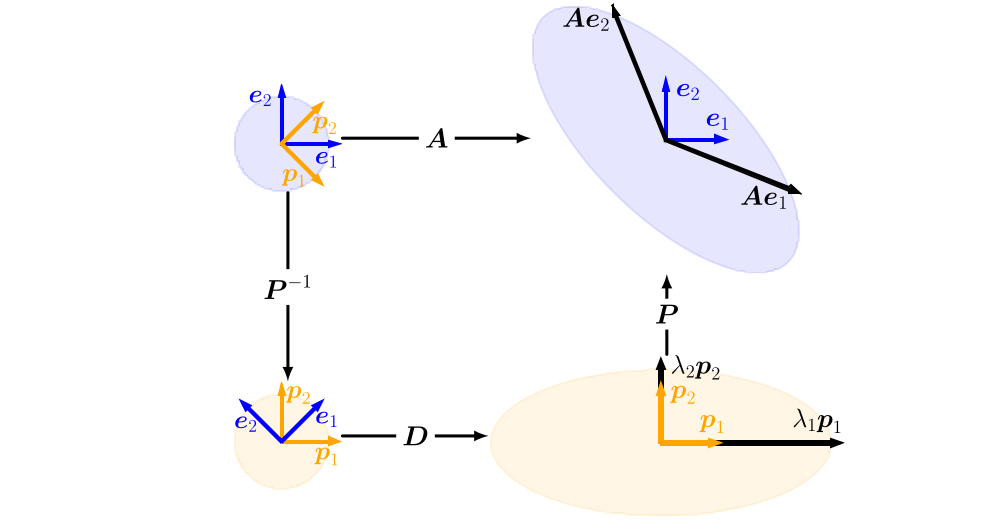
\includegraphics[width=10cm]{20}\\
\centering
\begin{itemize}
\item First $\bm{P}^{-1}$ performs a basis change from the standard basis into the eigenbasis. 
\item Then, the diagonal matrix $\bm{D}$ scales the vectors along these axes by the eigenvalues $\lambda_i$. 
\item Finally, $\bm{P}$ transforms these
scale vectors back into the standard/canonical coordinates.\\
\end{itemize}
\end{figure}\\
\textbf{Example}\\
Consider computing the eigendecomposition of $\bm{A}=
\frac{1}{2}\begin{bmatrix}
5&-2\\-2&5\end{bmatrix}$\\
\textbf{Step 1: Compute eigenvalues and eigenvectors}\\
The characteristic polynomal of $\bm{A}$ is 
\begin{align*}
\text{det}(\bm{A}-\lambda\bm{I})=\text{det}\left(\begin{bmatrix}
\frac{5}{2}-\lambda&-1\\-1&\frac{5}{2}-\lambda
\end{bmatrix}\right)
=\left(\lambda-\frac{7}{2}\right)\left(\lambda-\frac{3}{2}\right)
\end{align*}
The eigenvalues of $\bm{A}$ are $\lambda_1=\frac{7}{2}$ and $\lambda_2=\frac{3}{2}$ (the roots of the characteristic
polynomial). The associated normalised eigenvectors can then be obtained:
\begin{equation*}
\bm{p}_1=\frac{1}{\sqrt{2}}\begin{bmatrix}1\\-1\end{bmatrix},\quad
\bm{p}_2=\frac{1}{\sqrt{2}}\begin{bmatrix}1\\1\end{bmatrix}
\end{equation*}
Note that because of the spectral theorem an orthonormal basis exists. (normalisation or projection methods
may be required)\\
(next page)
\newpage
\noindent\textbf{Step 2: Check for existence}\\
The eigenvectors $\bm{p}_1,\bm{p}_2$ form a basis of 
$\mathbb{R}^2$. Therefore, $\bm{A}$ can be diagonalised.
(in this case the spectral theorem also gaurantees the existence of eigenvalues forming an ONB)\\
\vspace{1mm}\\
\textbf{Step 3: Construct the matrix $\bm{P}$ to diagonalise $\bm{A}$}\\
We collect the eigenvectors of $\bm{A}$ in $\bm{P}$:
\begin{equation*}
\bm{P}=[\bm{p}_1,\bm{p}_2]=\frac{1}{\sqrt{2}}
\begin{bmatrix}
1&1\\-1&1\end{bmatrix}
\end{equation*}
we also have our diagonal matrix where the diagonal elements are the eigenvalues:
\begin{equation*}
\bm{D}=\begin{bmatrix}
\frac{7}{2}&0\\0&\frac{3}{2}\end{bmatrix}
\end{equation*}
We now have our eigendecomposition $\bm{A}=\bm{PDP}^{-1}$:
\begin{equation*}
\underbrace{\frac{1}{2}\begin{bmatrix}5&-2\\-2&5\end{bmatrix}}_{\bm{A}}
=\underbrace{\frac{1}{\sqrt{2}}\begin{bmatrix}1&1\\-1&1\end{bmatrix}}_{\bm{P}}
\underbrace{\begin{bmatrix}\frac{7}{2}&0\\0&\frac{3}{2}\end{bmatrix}}_{\bm{D}}
\underbrace{\frac{1}{\sqrt{2}}\begin{bmatrix}1&-1\\1&1\end{bmatrix}}_{\bm{P}^{-1}}
\end{equation*}
\textbf{Significance of Eigendecomposition}\\
The value of Eigendecompostion comes from the ease of computation of diagonal matrices:
\begin{itemize}
\item Diagonal matrices $\bm{D}$ can efficiently be raised to a power. This allows us to easily find the matrix
power for a matrix $\bm{A}\in\mathbb{R}^{n\times n}$ via
eigendecomposition (since taking the power of a diagonal matrix is just the power of the diagonal elements):
\begin{equation*}
\bm{A}^k=(\bm{PDP}^{-1})^k=\bm{PD}^k\bm{P}^{-1}
\end{equation*}
Since computing $\bm{D}^k$ is efficient.
\item Assuming that the eigendecomposition $\bm{A}=\bm{PDP}^{-1}$ exists, then
\begin{align*}
\text{det}(\bm{A})&=\text{det}(\bm{PDP}^{-1})=\text{det}(\bm{P})\,\text{det}(\bm{D})\,\text{det}(\bm{P}^{-1})\\
&=\text{det}(\bm{D})=\prod_{i}d_{ii}
\end{align*}
Since det$(\bm{P}^{-1})=\frac{1}{\text{det}(\bm{P})}$ and the determinant of a diagonal matrix is just the product
down the diagonal.
\end{itemize}
Note that eigenvalue decomposition requires square matrices. 
\newpage

\subsection{Singular Value Decomposition I}%090824
\textbf{Theorem} \textit{Let $\bm{A}=\in\mathbb{R}^{m\times n}$ be a rectangular matrix of rank 
$r\in[0,\text{min}(m,n)]$. The SVD of $\bm{A}$ is the decomposition of the form}
\begin{figure}[h]

\includegraphics[width=10cm]{21}\\
\centering
\begin{equation*}
\underbrace{\bm{A}}_{m\times n}=\underbrace{\bm{U}}_{m\times m}
\underbrace{\bm{\Sigma}}_{m\times n}\underbrace{\bm{V}^T}_{n\times n}
\end{equation*}
\begin{itemize}
\item\textit{with an orthogonal matrix $\bm{U}\in\mathbb{R}^{m\times m}$ 
with column vectors\\ $\bm{u}_i,i=1,\ldots,m$,
\item an orthogonal matrix $\bm{V}\in\mathbb{R}^{n\times n}$ with column vectors\\ $\bm{v}_j,j=1,\ldots,n$,
\item and a $m\times n$ matrix $\bm{\Sigma}$ with $\Sigma_{ii}=\sigma_i\geq0$ and $\Sigma_{ij}=0,i\neq j$.}
\end{itemize}
\end{figure}\\
The diagonal entries $\sigma_{i},i=1,\ldots,r$, of $\bm{\Sigma}$ are called the \textit{singular values}. 
The column vectors $\bm{u}_i$ are called the \textit{left-singular vectors}. 
The column vectors $\bm{v}_j$ are called the \textit{right-singular vectors}. (by convention the singular values are
ordered, meaning $\sigma_1\geq\sigma_2\geq\sigma_r\geq0$)
\\(next page)
\newpage
\noindent\textbf{Structure of the Singular value matrix $\bm{\Sigma}$}\\
The \textit{Singular value matrix} $\bm{\Sigma}$ is unique; observe that $\Sigma\in\mathbb{R}^{n\times n}$ is
rectangular, being the same size as $\bm{A}$. This means that $\bm{\Sigma}$ has a diagonal submatrix that contains
the singular values and needs additional zero padding outside the diagonal: if
$m>n$, then the matrix $\bm{\Sigma}$ has diagonal structure up to row $n$ and then consists of $\bm{0}^T$
row vectors from row $n+1$ to $m$ below so that
\begin{equation*}
\begin{bmatrix}
\sigma_1&0&0\\0&\ddots&0\\0&0&\sigma_n\\
0&\cdots&0\\\vdots&&\vdots\\0&\cdots&0
\end{bmatrix}
\end{equation*}
If $m<n$, the matrix $\bm{\Sigma}$ has diagonal structure up till column $m$ and columns that consist of 
$\bm{0}$ from $m+1$ to $n$ so that
\begin{equation*}
\Sigma=\begin{bmatrix}
\sigma_1&0&0&0&\cdots&0\\0&\ddots&0&\vdots&&\vdots\\
0&0&\sigma_m&0&\cdots&0
\end{bmatrix}
\end{equation*}
The SVD exists for any matrix $\bm{A}\in\mathbb{R}^{m\times n}$.\\
(next page)
\newpage
\noindent\textbf{Geometric intuition for the SVD}\\
The SVD can be interpreted as a decomposition of a corresponding linear mapping $\Phi:\mathbb{R}^n\to\mathbb{R}^n$ 
into three operations. Assume we are given a transformation matrix of a linear mapping 
$\Phi:\mathbb{R}^n\to\mathbb{R}^m$ with respect to the standard bases $B$ and $C$ of $\mathbb{R}^n$ and 
$\mathbb{R}^m$ respectively; moreover, assume a second basis $\tilde{B}$ of $\mathbb{R}^n$ and $\tilde{C}$ of 
$\mathbb{R}^m$. Then
\begin{figure}[h]
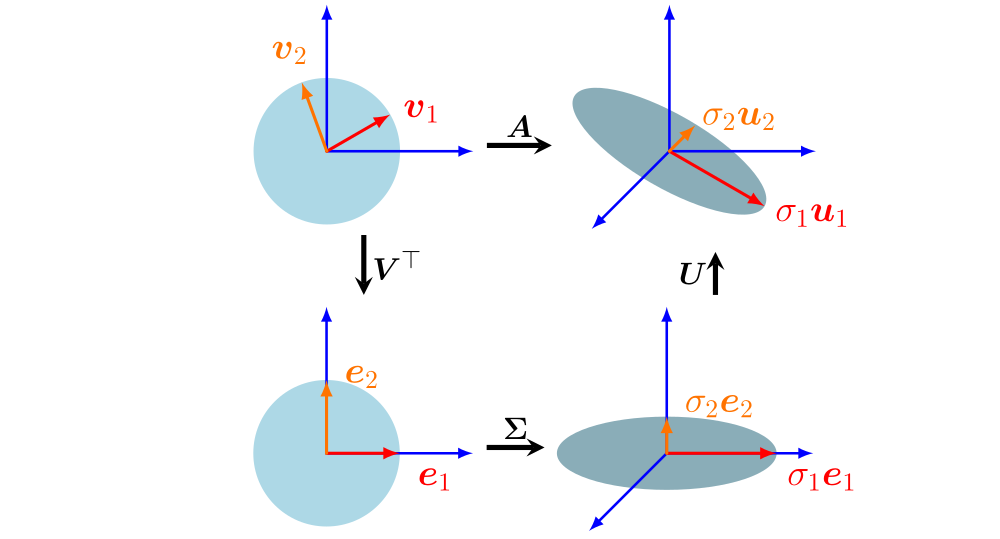
\includegraphics[width=10cm]{22}\\
\centering
\begin{enumerate}
\item The matrix $\bm{V}$ performs a basis change in the domain
$\mathbb{R}^n$ from $\tilde{B}$ (represented 
by the red and orange vectors $v_1$ and $v_2$ in the top-left figure) to the standard basis $B$ 
(since we set $B$ to be the standard basis).
$\bm{V}^T=\bm{V}^{-1}$ performs a basis change from $B$ to $\tilde{B}$. 
(since $\bm{V}$ is defined as an orthogonal matrix). (The red and orange vectors are now aligned with the
standard basis in the bottom left figure.)
\item Having changed the coordinate system to $\tilde{B}$, $\bm{\Sigma}$ scales the new coordinates by the singular
values $\sigma_i$ (and adds or deletes dimensions); as
with eigendecomposition, $\Sigma$ can be viewed as the transformation matrix of $\Phi$ with respect to $\tilde{B}$
and $\tilde{C}$ (represented by the red and orange vectors being stretched, lying in the $\bm{e}_1\bm{e}_2$ plane, 
which is now embedded in a third dimension (bottom right figure).
\item $\bm{U}$ performs a basis change in the codomain $\mathbb{R}^m$ from $\tilde{C}$ into the basis of 
$\mathbb{R}^m$, represented by the rotation of the red and orange vectors out of the $\bm{e}_1\bm{e}_2$ plane
(top right).
\end{enumerate}
\end{figure}\\
The SVD expresses a change of basis in both the domain and the codomain. This is in contrast with eigendecomposition
which operates within the same vector space, where the same basis change is applied and then undone.
What makes the SVD special is that these are two different bases linked by the singular value matrix $\Sigma$.\\
(next page)
\newpage
\noindent\textbf{Example}\\
Consider the mapping of a square grid of vectors $\bm{\chi}\in\mathbb{R}^2$ that fit a box centered at the origin.
Using the standard basis, we map these vectors using
\begin{align*}
\bm{A}&=\begin{bmatrix}1&-0.8\\0&1\\1&0\end{bmatrix}
=\bm{U\Sigma V}^T\\
&=\begin{bmatrix}-0.79&0&-0.62\\0.38&-0.78&-0.49\\
-0.48&-0.62&0.62\end{bmatrix}\begin{bmatrix}
1.62&0\\0&1.0\\0&0\end{bmatrix}\begin{bmatrix}
-0.78&0.62\\-0.62&-0.78\end{bmatrix}
\end{align*}
\begin{figure}[h]
\begin{center}
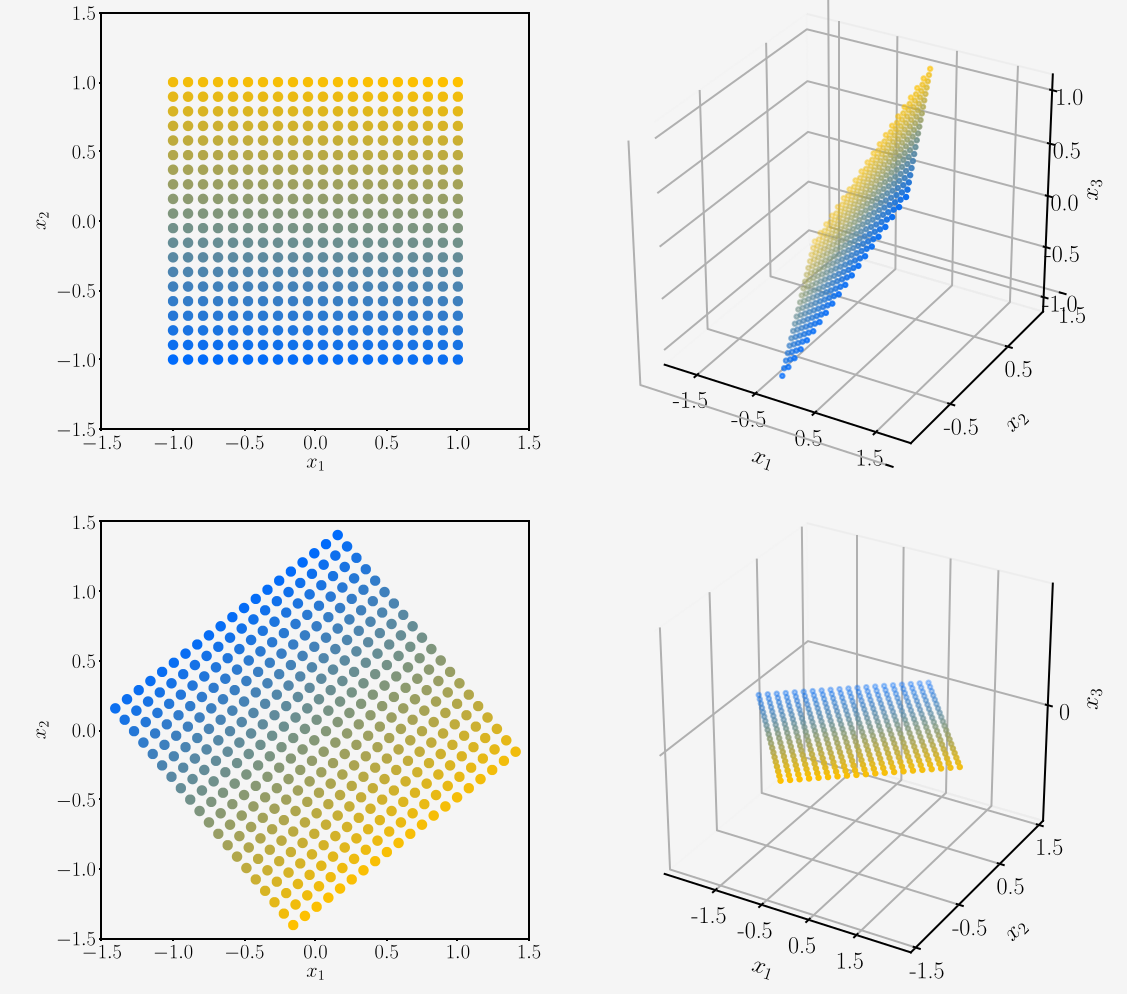
\includegraphics[width=10cm]{23}\\
\end{center}
We start with a set of vectors $\bm{\chi}$ (top left, arranged in a grid). Applying 
$\bm{V}^T\in\mathbb{R}^{2\times2}$ rotates $\bm{\chi}$
(bottom left). The singular value matrix $\bm{\Sigma}$
then
maps these vectors to the codomain $\mathbb{R}^3$ (bottom right); note that up till now all these vectors lie in the
$x_1x_2$ plane; the third coordinate is always zero, and the vectors in the $x_1x_2$ plane have been stretched by
the singular values.\\
\vspace{1mm}\\
Finally $\bm{U}$ performs a rotation within the codomain $\mathbb{R}^3$; now the mapped vectors are no longer
restricted to the $x_1x_2$ plane, but instead a different plane (top right).
\end{figure}
\newpage

\subsection{Singular Value Decomposition II} %120824
\textbf{SVD and Eigendecomposition}\\
Compare the eigendecomposition of an SPD (symmetric positive definite) matrix
\begin{equation*}
\bm{S}=\bm{S}^T=\bm{PDP}^T
\end{equation*}
with the corresponding SVD
\begin{equation*}
\bm{S}=\bm{U\Sigma V}^T
\end{equation*}
see that if we set
\begin{equation*}
\bm{U}=\bm{P}=\bm{V},\quad\bm{D}=\bm{\Sigma} 
\end{equation*}
the SVD of the SPD matrix is its eigendecomposition.\\
\vspace{1mm}\\
\textbf{Construction of the SVD (intuition)}\\
We begin with constructing the right-singular vectors. The spectral theorem tells us that the eigenvectors of a
symmetric matrix form an ONB (which is also non-defective and therefore can undergo eigendecomposition). 
Since we can always construct a symmetric, positive semidefinite matrix $\bm{A}^T\bm{A}\in\mathbb{R}^{n\times n}$ 
from any rectangular matrix $\bm{A}\in\mathbb{R}^{m\times n}$, we can always diagonalise
$\bm{A}^T\bm{A}$ and obtain
\begin{equation*}
\bm{A}^T\bm{A}=\bm{PDP}^T=\bm{P}\begin{bmatrix}
\lambda_1&\cdots&0\\\vdots&\ddots&\vdots\\0&\cdots
&\lambda_n
\end{bmatrix}\bm{P}^T
\end{equation*}
Where $\bm{P}$ is an orthogonal matrix (because $\bm{A}^T\bm{A}$ is symmetric and has eigenvalues that can form
an ONB). The $\lambda_i\geq0$ are the eigenvalues of $\bm{A}^T\bm{A}$; assuming that the SVD of $\bm{A}$
exists:
\begin{equation*}
\bm{A}^T\bm{A}=(\bm{U}\bm{\Sigma}\bm{V}^T)^T(\bm{U}\bm{\Sigma}\bm{V}^T)
=\bm{V}\bm{\Sigma}^T\bm{U}^T\bm{U}\bm{\Sigma}\bm{V}^T
\end{equation*}
Where $\bm{U},\bm{V}$ are orthogonal matrices (as defined in the SVD); therefore with $\bm{U}^T\bm{U}=\bm{I}$ we
obtain
\begin{equation*}
\bm{A}^T\bm{A}=\bm{V}\bm{\Sigma}^T\bm{\Sigma}\bm{V}^T
=\bm{V}\begin{bmatrix}
\sigma^2_1&\cdots&0\\\vdots&\ddots&\vdots\\0&\cdots&
\sigma^2_n
\end{bmatrix}\bm{V}^T
\end{equation*}
Comparing the two equations we get
\begin{align*}
\bm{V}^T&=\bm{P}^T\\
\sigma_i^2&=\lambda_i
\end{align*}
Therefore, the eigenvectors of $\bm{A}^T\bm{A}$ that compose $\bm{P}$ are the right-singular vectors $\bm{V}$ of
$\bm{A}$; the eigenvalues of $\bm{A}^T\bm{A}$ are the squared singular values of $\bm{\Sigma}$.\\
(next page)
\newpage
\noindent\textbf{Construction of the SVD (cont.)}\\
To obtain the left-singular vectors $\bm{U}$, we follow a similar procedure; notice that for
a different symmetric matrix $\bm{AA}^T\in\mathbb{R}^{m\times m}$ (instead of the previous 
$\bm{A}^T\bm{A}\in\mathbb{R}^{n\times n}$), we have
\begin{align*}
\bm{AA}^T&=(\bm{U}\bm{\Sigma}\bm{V}^T)(\bm{U}\bm{\Sigma}\bm{V}^T)^T=
\bm{U}\bm{\Sigma}\bm{V}^T\bm{V\Sigma}^T\bm{U}^T\\
&=\bm{U}\begin{bmatrix}
\sigma^2_1&\cdots&0\\\vdots&\ddots&\vdots\\0&\cdots&
\sigma^2_m
\end{bmatrix}\bm{U}^T
\end{align*}
since $\bm{AA}^T$ is also a symmetric matrix (different from $\bm{A}^T\bm{A}$, notice they have different sizes 
for $m\neq n$), the spectral theorem tells us that as before, it can be diagonalised and an ONB of eigenvectors
of $\bm{AA}^T=\bm{SDS}^T$ can be found and collected in $\bm{S}$; the orthonormal eigenvectors of $\bm{AA}^T$ are
the left-singular vectors $\bm{U}$ and form an orthonormal basis in the codomain of the SVD.\\
\vspace{1mm}\\
Also notice that $\bm{\Sigma}$ remains the same for both cases (since we use the SVD of $\bm{A}$), thus the nonzero
entries $\sigma_i$ in both cases are the same.\\
\vspace{1mm}\\
We finish the construction of the SVD by connecting the basis $\bm{U}$ to $\bm{V}$ using the fact that 
the images of the $\bm{v}_i$ under $\bm{A}$ have to be \textit{orthogonal}.
The inner product between $\bm{Av}_i$ and $\bm{Av}_j$ is 0 for $i\neq j$; for any two orthogonal eigenvectors
$\bm{v}_i,\bm{v}_j,\,i\neq j$, see that
\begin{equation*}
(\bm{Av}_i)^T(\bm{Av}_j)=\bm{v}_i^T(\bm{A}^T\bm{A})\bm{v}_j=
\bm{v}_i^T(\lambda_j\bm{v}_j)=\lambda_j\bm{v}_i^T\bm{v}_j=0
\end{equation*}
We need left-singular values that are \textit{orthonormal}, so we normalise the
images of the right-singular vectors $\bm{Av}_i$ and obtain (since the images of $\bm{v}_i$ under $\bm{A}$ are
orthogonal their normalisations are orthonormal)
\begin{equation*}
\bm{u}_i:=\frac{\bm{Av}_i}{||\bm{Av}_i||}=\frac{1}{\sqrt{\lambda_i}}\bm{Av}_i
=\frac{1}{\sigma_i}\bm{Av}_i
\end{equation*}
the last equality comes from the earlier finding that 
$\sigma_i^2=\lambda_i$. (point is that the normalisation factors turn out to be the singular values, 
connecting the orthonormal bases $\bm{U}$ and $\bm{V}$)\\
(next page)
\newpage
\noindent\textbf{Construction of the SVD (cont.)}\\
We had
\begin{equation*}
\bm{u}_i=\frac{1}{\sigma_i}\bm{Av}_i
\end{equation*}
which can be rearranged into the \textit{singular value equation}
\begin{equation*}
\bm{Av}_i=\sigma_i\bm{u}_i,\quad i=1,\ldots,r
\end{equation*}
(this equation closely resembles the eigenvalue equation, but the vectors on the left and right hand sides are not
the same)\\
\vspace{1mm}\\
Note that for $n<m$, this equation holds only for $i\leq n$, and says nothing about the $\bm{u}_i$ for $i>n$;
(since $\bm{u}_i$ where $i>n$ get scaled to 0)
however we know by construction that they are orthonormal.
Conversely, for $m<n$, the equation holds only for $i\leq m$; for $i>m$, we have $\bm{Av}_i=\bm{0}$ (as defined)
since $\bm{v}_i$ form an orthonormal set; this means that
the SVD also supplies an orthonormal basis of the kernel
of $\bm{A}$.
\newpage

\subsection{Computing the SVD (Example)}%130824
Consider finding the singular value decomposition of
\begin{equation*}
\bm{A}=\begin{bmatrix}1&0&1\\
-2&1&0\end{bmatrix}
\end{equation*}
the SVD requires us to compute the right-singular vectors $\bm{v}_j$, the singular values $\sigma_k$, and the
left-singular vectors $\bm{u}_i$.\\
\vspace{1mm}\\
\textbf{Step 1: Right-singular vectors as the eigenbasis of $\bm{A}^T\bm{A}$}\\
We start by computing 
\begin{equation*}
\bm{A}^T\bm{A}=\begin{bmatrix}
1&-2\\0&1\\1&0
\end{bmatrix}\begin{bmatrix}
1&0&1\\-2&1&0\end{bmatrix}=\begin{bmatrix}
5&-2&1\\-2&1&0\\1&0&1
\end{bmatrix}
\end{equation*}
Now we compute the singular values and right-singular values through eigendecomposition of $\bm{A}^T\bm{A}$,
given as
\begin{equation*}
\bm{A}^T\bm{A}=\begin{bmatrix}
\frac{5}{\sqrt{30}}&0&\frac{-1}{\sqrt{6}}\\
\frac{-2}{\sqrt{30}}&\frac{1}{\sqrt{5}}&\frac{-2}{\sqrt{6}}\\
\frac{1}{\sqrt{30}}&\frac{2}{\sqrt{5}}&\frac{1}{\sqrt{6}}
\end{bmatrix}\begin{bmatrix}6&0&0\\0&1&0\\0&0&0
\end{bmatrix}\begin{bmatrix}
\frac{5}{\sqrt{30}}&\frac{-2}{\sqrt{30}}&\frac{1}{\sqrt{30}}\\
0&\frac{1}{\sqrt{5}}&\frac{2}{\sqrt{5}}\\
\frac{-1}{\sqrt{6}}&\frac{-2}{\sqrt{6}}&\frac{1}{\sqrt{6}}
\end{bmatrix}=\bm{PDP}^T
\end{equation*}
We obtain the right singular vectors as the columns of $\bm{P}$ so that
\begin{equation*}
\bm{V}=\bm{P}=\begin{bmatrix}
\frac{5}{\sqrt{30}}&0&\frac{-1}{\sqrt{6}}\\
\frac{-2}{\sqrt{30}}&\frac{1}{\sqrt{5}}&\frac{-2}{\sqrt{6}}\\
\frac{1}{\sqrt{30}}&\frac{2}{\sqrt{5}}&\frac{1}{\sqrt{6}}
\end{bmatrix}
\end{equation*}
\textbf{Step 2: Singular value matrix}\\
As the singular values $\sigma_i$ are the square roots of the eigenvalues of 
$\bm{A}^T\bm{A}$ we obtain them straight from $\bm{D}$.
Since rk($\bm{A}=2$), there are only two nonzero singular values $\sigma_1=\sqrt{6}$ and $\sigma_2=1$.
The singular value matrix must be the same size as $\bm{A}$, and we obtain
\begin{equation*}
\bm{\Sigma}=\begin{bmatrix}
\sqrt{6}&0&0\\0&1&0
\end{bmatrix}
\end{equation*}
(next page)
\newpage
\noindent\textbf{Step 3: Left-singular vectors as normalised image of right singular vectors}\\
We find the left-singular vectors by computing the image of the right-singular vectors under $\bm{A}$ and
normalising them by dividing them by their corresponding singular value; we obtain
\begin{align*}
\bm{u}_1&=\frac{1}{\sigma_1}\bm{Av}_1=\frac{1}{\sqrt{6}}
\begin{bmatrix}1&0&1\\
-2&1&0\end{bmatrix}\begin{bmatrix}
\frac{5}{\sqrt{30}}\\\frac{-2}{\sqrt{30}}\\\frac{1}{\sqrt{30}}
\end{bmatrix}=\begin{bmatrix}
\frac{1}{\sqrt{5}}\\\frac{-2}{\sqrt{5}}\end{bmatrix}\\
\bm{u}_2&=\frac{1}{\sigma_2}\bm{Av}_2=\frac{1}{1}
\begin{bmatrix}1&0&1\\
-2&1&0\end{bmatrix}\begin{bmatrix}
0\\\frac{1}{\sqrt{5}}\\\frac{2}{\sqrt{5}}\end{bmatrix}
=\begin{bmatrix}
\frac{2}{\sqrt{5}}\\\frac{1}{\sqrt{5}}\end{bmatrix}\\
\bm{U}&=[\bm{u}_1,\bm{u}_2]=\frac{1}{\sqrt{5}}
\begin{bmatrix}1&2\\-2&1\end{bmatrix}
\end{align*}
(On a computer the approach illustrated here has poor numerical behaviour, and the SVD of $\bm{A}$ is normally
computed without resorting to eigenvalue decomposition of 
$\bm{A}^T\bm{A}$.)
\newpage

\subsection{$\bm{A}^T\bm{A}$ and $\bm{AA}^T$ possess the
same nonzero eigenvalues}
Show that for any $\bm{A}\in\mathbb{R}^m\times n$ the matrices $\bm{A}^T\bm{A}$ and $\bm{AA}^T$ possess the
same nonzero eigenvalues. Consider an eigenvalue 
$\lambda\neq0$ of $\bm{A}^T\bm{A}$; meaning there exists
$\bm{x}\in\mathbb{R}^n$ such that
\begin{equation*}
\bm{A}^T\bm{A}\bm{x}=\lambda\bm{x}
\end{equation*}
now see that
\begin{equation*}
\bm{A}\bm{A}^T\bm{A}\bm{x}=\lambda\bm{A}\bm{x}
\end{equation*}
the eigenvector changed but the eigenvalue did not. 
\newpage

\subsection{Eigenvalue Decomposition vs. \\Single Value Decomposition---Summary}%130824
Here we review the core elements of the eigendecomposition
$\bm{A}=\bm{PDP}^{-1}$ and the SVD $\bm{A}=\bm{U\Sigma V}^T$.
\begin{itemize}
\item The SVD always exists for any matrix $\mathbb{R}^{m\times n}$. The eigendecomposition is only defined for
square matrices $\mathbb{R}^{n\times n}$ and only exists if we can find a basis of eigenvectors of $\mathbb{R}^n$.
\item The vectors in the eigendecomposition matrix $\bm{P}$ are not necessarily orthogonal (the change of
nasis is not a simple rotation and scaling). On the other hand, the vectors in the matrices $\bm{U}$ and $\bm{V}$
in the SVD are orthonormal, so they represent rotations.
\item Both the eigendecomposition and the SVD are compositions of three linear mappings:
\begin{enumerate}
\item Change of basis in the domain
\item Independent scaling of each new basis vector and mapping from domain to codomain
\item Change of basis in the codomain
\end{enumerate}
The difference here is that in the SVD, domain and codomain can be vector spaces of different dimensions.
\item In the SVD, the left and right singular vector matrices $\bm{U}$ and $\bm{V}$ are generally not inverse of
each other (since they perform basis changes in different vector spaces, and are of different sizes). 
In the eigendecomposition, the basis change matrices $\bm{P}$ and $\bm{P}^{-1}$ are inverses of each other.
\item In the SVD, the entries in the diagonal matrix $\bm{\Sigma}$ are all real and non-negative
(due to the spectral theorem and the symmetry of $\bm{A}^T
\bm{A}$), which is
generally not true for the diagonal matrix in eigendecompostion.
\item The SVD and the eigendecomposition are closely related through their projections:
\begin{itemize}
\item The left singular vectors of $\bm{A}$ are the eigenvectors of $\bm{AA}^T$
\item The right singular vectors of $\bm{A}$ are eigenvectors of $\bm{A}^T\bm{A}$
\item The nonzero singular values of $\bm{A}$ are the square roots of the nonzero eigenvalues of both
$\bm{AA}^T$ and $\bm{A}^T\bm{A}$.
\end{itemize}
\item For symmetric matrices matrices $\bm{A}=\in\mathbb{R}^{n\times n}$, the eigenvalue decomposition and the SVD
are one and the same, which follows from the spectral theorem.
\end{itemize}
\newpage

\subsection{Matrix Approximation}%140824
\textbf{Intuituion}\\
The SVD allows for factorisation of $\bm{A}\in\mathbb{R}^{m\times n}$ into the product of three matrices 
\begin{equation*}
\bm{A}=\bm{U\Sigma V}^T
\end{equation*}
where $\bm{U}\in\mathbb{R}^{m\times m}$ and $\bm{V}\in\mathbb{R}^{n\times n}$ are orthogonal and 
$\bm{\Sigma}$ contains the singular values on its main diagonal.\\
\vspace{1mm}\\
\textbf{Rank-1 Matrices}\\
We can construct a rank-1 matrix $\bm{A}_i\in\mathbb{R}^{m\times n}$ as 
\begin{equation*}
\bm{A}_i:=\bm{u}_i\bm{v}_i^T
\end{equation*}
which is formed by the outer product of the $i$th orthogonal column vector of $\bm{U}$ and $\bm{V}$. Now see that,
corresponding with the SVD, a matrix $\bm{A}\in\mathbb{R}^{m\times n}$ of rank $r$ can be written as a sum of
rank-1 matrices $\bm{A}_i$ so that 
\begin{equation*}
\bm{A}=\sum^r_{i=1}\sigma_i\bm{u}_i\bm{v}_i^T=
\sum^r_{i=1}\sigma_i\bm{A}_i
\end{equation*}
(visualise the SVD and notice that this is essentially the same)
where the outer-product matrices $\bm{A}_i$ are weighted by the $i$th singular value $\sigma_i$; the diagonal
structure of the singular value matrix $\bm{\Sigma}$ multiplies only matching left and right singular vectors
$\bm{u}_i\bm{v}_i^T$ and scales them by their corresponding singular value $\sigma_i$. Illustrated:
\begin{figure}[h]
\begin{center}

\includegraphics[width=9.5cm]{24}\\
\end{center}
The original greyscale image is a $1432\times1910$ matrix of values between 0 (black) and 1 (white). 
(b) to (f) illustrate a few rank-1 matrices $\bm{A}_1,\ldots,\bm{A}_5$ and their corresponding singular values
$\sigma_1,\ldots,\sigma_5$. Each matrix is formed by the outer-product of the left and right singular vectors.\\
(next page)
\end{figure}
\newpage
\noindent\textbf{Approximation}\\
Since summing up the $r$ individual rank-1 matrices gives the rank-$r$ matrix $\bm{A}$, 
if the sum dows not run over all matrices $\bm{A}_i,i=1,\ldots,r$, but only up to an intermediate value $k<r$, 
we obtain a \textit{rank-k approximation}
\begin{equation*}
\widehat{\bm{A}}(k):=\sum^k_{i=1}\sigma_i\bm{u}_i\bm{v}_i^T=\sum^k_{i=1}\sigma_i\bm{A}_i
\end{equation*}
of $\bm{A}$ with rk$(\widehat{\bm{A}}(k))=k$.\\
\vspace{1mm}\\
Applied:
\begin{figure}[h]
\begin{center}

\includegraphics[width=10cm]{25}\\
\end{center}
Illustrated are low-rank approximations $\widehat{\bm{A}}(k)$ of an original image $\bm{A}$. The details of
the image become increasingly recognisable in the rank-5
approximation. While the original image requires storage of $1432\cdot1910=2735120$ numbers, the rank-5
approximation only requires the storage of the five singular values and the five left and right singular vectors
($1432\times1$ and $1\times1910$ each) for a total of 
$5\cdot(1432+1910+1)=16715$ numbers---about $0.6\%$ of the original.
\end{figure}
\newpage

\subsection{Spectral Norm, Eckart-Young theorem}
\textbf{Spectral Norm}\\
For $\bm{x}\in\mathbb{R}^n\backslash\{\bm{0}\}$, the \textit{spectral norm} of a matrix 
$\bm{A}\in\mathbb{R}^{m\times n}$ is defined as
\begin{equation*}
||\bm{A}||_2:=\max_{\bm{x}}\frac{||\bm{Ax}||_2}{||\bm{x}||_2}
\end{equation*}
The spectral norm essentially determines how long any vector $\bm{x}$ can at most become when 
multiplied by $\bm{A}$.\\
\vspace{1mm}\\
\textbf{Spectral norm and Singular values}\\
Theorem: \textit{The spectral norm of $\bm{A}$ is its largest singular value $\sigma_1$.}\\
\vspace{1mm}\\
This can be seen from the SVD formula, where 
\begin{equation*}
\bm{Ax}=\bm{U\Sigma V}^T\bm{x}
\end{equation*}
$\bm{U}$ and $\bm{V}^T$ are orthogonal matrices and therefore leave the norm unchanged. 
This leaves the `scaling matrix' $\bm{\Sigma}$, where (by convention all $\sigma_i\geq0$) the 
largest scaling factor is the largest singular value $\sigma_1$.\\
\vspace{1mm}\\
\textbf{Eckart-Young Theorem}\\
Theorem: \textit{Consider a matrix $\bm{A}\in\mathbb{R}^{m\times n}$ of rank $r$ and let 
$\bm{B}\in\mathbb{R}^{m\times n}$ be a matrix of rank $k$.
For any $k\leq r$ with $\widehat{\bm{A}}(k)=
\sum^k_{i=1}\sigma_i\bm{u}_i\bm{v}_i^T$ it holds that}
\begin{align*}
\widehat{\bm{A}}(k)&=\text{argmin}_{\text{rk}(\bm{B})=k}
||\bm{A}-\bm{B}||_2\\
||\bm{A}-\widehat{\bm{A}}(k)||_2&=\sigma_{k+1}
\end{align*}
The Eckart-Young theorem states explicitly how much error we introduce by approximating $\bm{A}$ using a rank-$k$
approximation; we can interpret the rank-k approximation obtained with the SVD as a projection of the full rank
matrix $\bm{A}$ onto a lower-dimensional space of rank-at-most-$k$ matrices. Of all possible projections, the 
SVD minimises the error rate (with respect to the spectral norm) between $\bm{A}$ and any rank-k approximation.\\
\vspace{1mm}\\
\textbf{Intuition for formula}\\
Observe that the difference $\bm{A}-\widehat{\bm{A}}(k)$ is a matrix containing the sum of the remaining rank-1 
matrices
\begin{equation*}
\bm{A}-\widehat{\bm{A}}(k)=\sum^r_{i=k+1}\sigma_i\bm{u}_i\bm{v}_i^T
\end{equation*}
We immediately obtain $\sigma_{k+1}$ as the spectral norm of the difference matrix.\\
(next page)
\newpage
\noindent\textbf{More intuition}\\
Of all possible projections, the SVD minimises the error rate (with respect to the spectral norm)
between $\bm{A}$ and any rank-k approximation. Say that this isn't the case and there is 
another matrix $\bm{B}$ with $\text{rk}(\bm{B})\leq k$, such that
\begin{equation*}
||\bm{A}-\bm{B}||<||\bm{A}-\widehat{\bm{A}}(k)||_2
\end{equation*}
(meaning that there exists an approximation with less error than the matrix approximation) then there exists 
an at least $(n-k)$-dimensional null space $Z\subseteq\mathbb{R}^n$, such that $\bm{x}\in Z$ implies that
$\bm{Bx}=\bm{0}$. Then it follows that
\begin{equation*}
||\bm{Ax}||_2=||(\bm{A}-\bm{B})\bm{x}||_2
\end{equation*}
by using a version of the Cauchy-Schwartz inequality that encompasses norms of matrices, we obtain
\begin{equation*}
||\bm{Ax}||_2=\underbrace{||(\bm{A}-\bm{B})\bm{x}||_2
<||(\bm{A}-\bm{B})||_2\,||\bm{x}||_2}_{\text{Cauchy-Schwartz}}<\sigma_{k+1}||\bm{x}||_2
\end{equation*}
(the last inequality comes from our assumption that 
$||\bm{A}-\bm{B}||<||\bm{A}-\widehat{\bm{A}}(k)||_2=\sigma_{k+1}$)\\
\vspace{1mm}\\
However, there exists a $(k+1)$-dimensional subspace where
$||\bm{Ax}||_2\geq\sigma_{k+1}||\bm{x}||_2$, which is 
spanned by the right-singular vectors $\bm{v}_j,j\leq
k+1$ of $\bm{A}$. Adding up the dimensions of these two spaces yields a number greater than $\bm{n}$, which is a 
contradiction of the rank-nullity theorem.\\
\vspace{1mm}\\
\textbf{Significance of Eckart-Young Theorem}\\
The Eckart-Young Theorem implies that we can use the SVD to reduce a rank-$r$ matrix $\bm{A}$ to a rank-$k$ matrix
in a principled, optimal manner. We can interpret the approximation of $\bm{A}$ by a rank-$k$ matrix as a form of
lossy compression.
\newpage

\subsection{Matrix Phylogeny (Summary of Chapters)}%180824
Illustrated is a fundamental phylogenic tree of matrices and linear mappings:
\begin{figure}[h]
\begin{center}
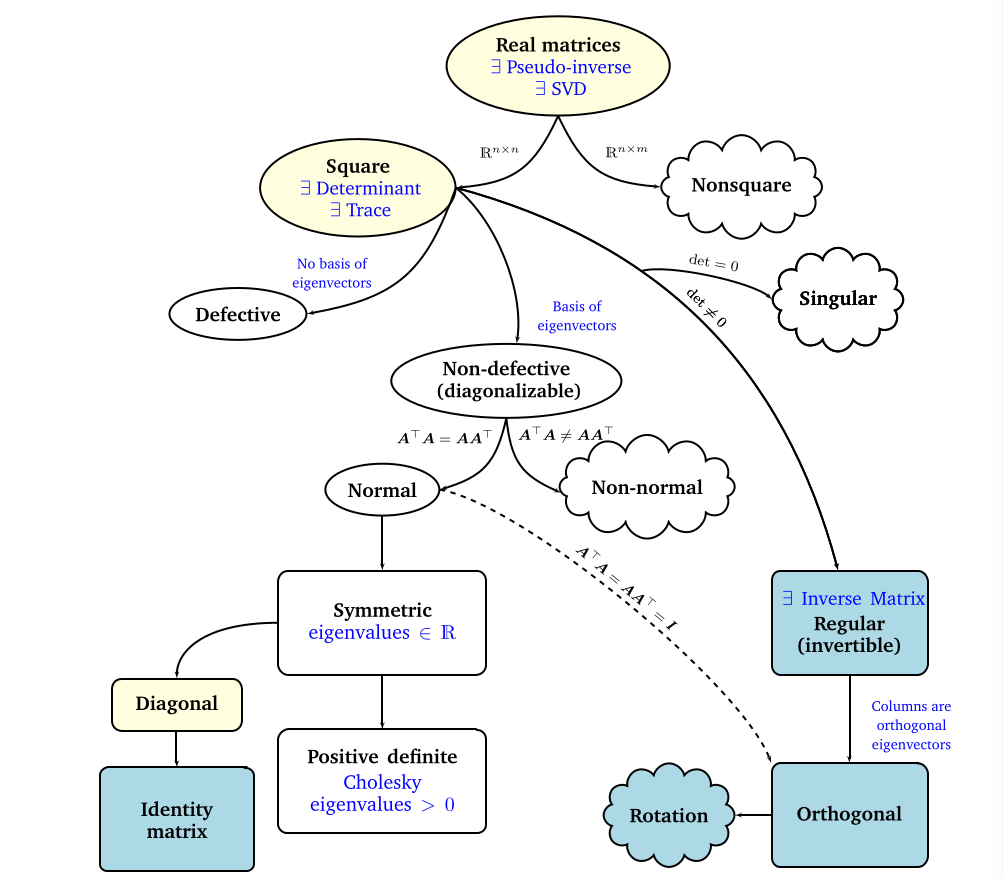
\includegraphics[width=10cm]{26}\\
\end{center}
We consider all \textit{real matrices} $\bm{A}\in\mathbb{R}^{n\times m}$; for non-square matrices the SVD always exists.\\
\vspace{1mm}\\
\textbf{Square matrices}\\
Focusing on \textit{square matrices} $\bm{A}\in\mathbb{R}^{n\times n}$ the \textit{determinant} tells one whether 
a square matrix possesses an \textit{inverse matrix}. 
If the square $n\times n$ matrix possesses $n$ linearly independent eigenvectors, then the matrix is non-defective
and an \textit{eigendecomposition} exists. We know that repeated eigenvalues may result in defective matrices,
which cannot be diagonalised. (note that non-singular/non-invertible matrices and non-defective matrices are not
the same)\\
(next page)
\end{figure}
\newpage
\noindent\textbf{Normal, Orthogonal matrices}\\
For non-defective square $n\times n$ matrices, $\bm{A}$ is \textit{normal} if the contition 
$\bm{A}^T\bm{A}=\bm{AA}^T$ holds. Moreover, if the more restrictive condition holds that $\bm{A}^T\bm{A}=\bm{AA}^T
=\bm{I}$, then $\bm{A}$ is called \textit{orthogonal}; the set of orthogonal matrices is a subset of the regular
(invertible) matrices and satisfy $\bm{A}^T=\bm{A}^{-1}$.
\\
\vspace{1mm}\\
\textbf{Symmetric Matrices, Symmetric Positive definite Matrices}\\
Normal matrices have a frequently encountered subset---the symmetric matrices $\bm{S}\in\mathbb{R}^n\times n$,
which satisfy $\bm{S}=\bm{S}^T$. Symmetric matrices have 
only real eigenvalues (spectral theorem). A subset of the symmetric matrices consists of the positive definite
matrices $\bm{P}$ which satisfy the condition of $\bm{x}^T\bm{Px}>0$ for all $\bm{x}\in\mathbb{R}^n\backslash\{\bm{0}\}$; in this case, a unique 
\textit{Cholesky decomposition} exists. Positive definite matrices have only positive eigenvalues and are always
invertible.\\
\vspace{1mm}\\
\textbf{Diagonal matrices}\\
Another subset of symmetric matrices consists of the \textit{diagonal matrices} $\bm{D}$; diagonal matrices are
closed under multiplication and addition, but do not necessarily form a group. A special diagonal matrix is the
identity $\bm{I}$.
\newpage

\section{Vector Calculus}
\subsection{Partial Differentiation and Gradients}%290824
\textbf{Definition}\\
The generalisaion of the derivative to functions of several variables is the \textit{gradient}; the gradient of
function $f$ with respect to $x$ is found by \textit{varying one variable at a time} and keeping others constant. 
The gradient is then the collection of these \textit{partial derivatives}.\\
\vspace{1mm}\\
For a function $f:\mathbb{R}^n\to\mathbb{R},\,\bm{x}\mapsto f(x),\,\bm{x}\in\mathbb{R}^n$ we
define the \textit{partial derivatives} as
\begin{align*}
\frac{\partial f}{\partial x_1}&=\lim_{h\to0}
\frac{f(x_1+h,x_2,\ldots,x_n)-f(\bm{x})}{h}\\
&\vdots\\
\frac{\partial f}{\partial x_n}&=\lim_{h\to0}
\frac{f(x_1,\ldots,x_{n-1},x_n+h)-f(\bm{x})}{h}
\end{align*}
collecting them in a row vector we get
\begin{equation*}
\nabla_xf=\text{grad}f=\frac{df}{d\bm{x}}=
\begin{bmatrix}\frac{\partial f(\bm{x})}{\partial x_1}&
\frac{\partial f(\bm{x})}{\partial x_2}&\cdots&
\frac{\partial f(\bm{x})}{\partial x_n}
\end{bmatrix}\in\mathbb{R}^{1\times n}
\end{equation*}
this is called the \textit{gradient} of $f$ (it is also the \textit{Jacobian}, but note that this is a particular
case of the Jacobian, whose definition can apply more generally to vector-valued functions).
\newpage

\subsection{Chain Rule}%290824
\textbf{Definition and Vector notation}\\
Considering a function $f:\mathbb{R}^2\to\mathbb{R}$ of two variables $x_1x_2$, where $x_1(t)$ and $x_2(t)$ are
themselves functions of $t$, to compute the gradient of $f$ with respect to $t$ we apply the chain rule
for multivariate functions as
\begin{equation*}
\frac{df}{dt}=\begin{bmatrix}
\frac{\partial f}{\partial x_1}&\frac{\partial f}{\partial x_2}\end{bmatrix}
\begin{bmatrix}\frac{\partial x_1(t)}{\partial t}\\\frac{\partial x_2(t)}{\partial t}\end{bmatrix}
=\frac{\partial f}{\partial x_1}\frac{\partial x_1}{\partial t}+
\frac{\partial f}{\partial x_2}\frac{\partial x_2}{\partial t}
\end{equation*}
Consider another case where $f(x_1,x_2)$ is a function of $x_1$ and $x_2$, where $x_1(s,t)$ and $x_2(s,t)$ are
themselves functions of two variables $s$ and $t$, the chain rule yields
\begin{align*}
\frac{df}{ds}=\frac{\partial f}{\partial x_1}\frac{\partial x_1}{\partial s}+
\frac{\partial f}{\partial x_2}\frac{\partial x_2}{\partial s}\\
\frac{df}{dt}=\frac{\partial f}{\partial x_1}\frac{\partial x_1}{\partial t}+
\frac{\partial f}{\partial x_2}\frac{\partial x_2}{\partial t}
\end{align*}
expressed compactly in matrix notation we have
\begin{equation*}
\frac{df}{d(s,t)}=\frac{\partial f}{\partial\bm{x}}\frac{\partial\bm{x}}{\partial(s,t)}
=\underbrace{\begin{bmatrix}\frac{\partial f}{\partial x_1}&\frac{\partial f}{\partial x_2}\end{bmatrix}}_{=\frac{\partial f}{\partial\bm{x}}}
\underbrace{\begin{bmatrix}\frac{\partial x_1}{\partial s}&\frac{\partial x_1}{\partial t}\\
\frac{\partial x_2}{\partial s}&\frac{\partial x_2}{\partial t}
\end{bmatrix}}_{=\frac{\partial\bm{x}}{\partial(s,t)}}
\end{equation*}
\newpage

\subsection{Gradients of Vector-Valued Functions, the Jacobian}%290824
\textbf{Intuition}\\
Here we generalise the concept of the gradient to vector valued functions $\bm{f}:\mathbb{R}^n\to\mathbb{R}^m$, 
where $n\geq1$ and $m>1$. Considering a function $\bm{f}:\mathbb{R}^n\to\mathbb{R}^m$ and a vector
$\bm{x}=[x_1,\ldots,x_n]^T\in\mathbb{R}^n$, the corresponding vector of function values is given as
\begin{equation*}
\bm{f}(\bm{x})=\begin{bmatrix}f_1(\bm{x})\\\vdots\\
f_m(\bm{x})\end{bmatrix}\in\mathbb{R}^m
\end{equation*}
Writing the vector-valued function in this way allows us to view a vector-valued function $\bm{f}:\mathbb{R}^n
\to\mathbb{R}^m$ as a vector of functions $[f_1,\ldots,f_m]^T,\,f_i:\mathbb{R}^n\to\mathbb{R}$ that map 
onto $\mathbb{R}$.\\
\vspace{1mm}\\
Therefore, the partial derivative of a vector-valued function $\bm{f}:\mathbb{R}^n\to\mathbb{R}^m$ with respect 
to $x_i\in\mathbb{R},\,i=1,\ldots,n$, is given as the vector
\begin{equation*}
\frac{\partial\bm{f}}{\partial x_i}=\begin{bmatrix}
\frac{\partial f_1}{\partial x_i}\\\vdots\\
\frac{\partial f_m}{\partial x_i}\end{bmatrix}=
\begin{bmatrix}
\lim_{h\to0}\frac{f_1(x_1,\ldots,x_{i-1},x_i+h,x_{i+1},\ldots,x_n)-f_1(\bm{x})}{h}\\\vdots\\
\lim_{h\to0}\frac{f_m(x_1,\ldots,x_{i-1},x_i+h,x_{i+1},\ldots,x_n)-f_m(\bm{x})}{h}
\end{bmatrix}\in\mathbb{R}^m
\end{equation*}
The gradient of $\bm{f}$ with respect to a vector is the row vector of the partial derivatives, and every partial
derivative $\partial\bm{f}/\partial x_i$ is itself a column vector. Therefore we obtain the gradient of 
$\bm{f}:\mathbb{R}^n\to\mathbb{R}^m$ with respect to $\bm{x}\in\mathbb{R}^n$ by collecting these 
partial derivatives:
\begin{align*}
\frac{d\bm{f}(x)}{d\bm{x}}&=\begin{bmatrix}
\frac{\partial\bm{f}(\bm{x})}{\partial x_1}&\cdots&
\frac{\partial\bm{f}(\bm{x})}{\partial x_n}\end{bmatrix}\\
&=\begin{bmatrix}
\frac{\partial f_1(\bm{x})}{\partial x_1}&\cdots&
\frac{\partial f_1(\bm{x})}{\partial x_n}\\
\vdots&&\vdots\\
\frac{\partial f_m(\bm{x})}{\partial x_1}&\cdots&
\frac{\partial f_m(\bm{x})}{\partial x_n}
\end{bmatrix}\in\mathbb{R}^{m\times n}
\end{align*}
(next page)
\newpage
\noindent\textbf{The Jacobian}\\
The collection of all first-order partial derivatives of a vector-valued function 
$\bm{f}:\mathbb{R}^n\to\mathbb{R}^m$ is called the \textit{Jacobian}. The Jacobian $\bm{J}$ is an $m\times n$ 
matrix, which we define and arrange as follows:
\begin{align*}
\bm{J}&=\nabla_{\bm{x}}\bm{f}=\frac{d\bm{f}(x)}{d\bm{x}}=
\begin{bmatrix}\frac{\partial\bm{f}(\bm{x})}{\partial x_1}&\cdots&
\frac{\partial\bm{f}(\bm{x})}{\partial x_n}\end{bmatrix}\\
&=\begin{bmatrix}
\frac{\partial f_1(\bm{x})}{\partial x_1}&\cdots&
\frac{\partial f_1(\bm{x})}{\partial x_n}\\
\vdots&&\vdots\\
\frac{\partial f_m(\bm{x})}{\partial x_1}&\cdots&
\frac{\partial f_m(\bm{x})}{\partial x_n}
\end{bmatrix}\\
\text{where }\bm{x}&=\begin{bmatrix}x_1\\\vdots\\x_n
\end{bmatrix},\quad J(i,j)=\frac{\partial f_i}{\partial x_i}
\end{align*}
(see that a particular case of the Jacobian is that for a function $f:\mathbb{R}^n\to\mathbb{R}^1$, which 
possesses a Jacobian that is a row vector)\\
\vspace{1mm}\\
(Also note that the above notation of the Jacobian is termed the 
\textit{numerator layout} of the derivative, where the elements of $\bm{f}$ define the rows while the elements of 
$\bm{x}$ define the columns. There exists also a \textit{denominator layout}, which is the transpose of the
numerator layout.)\\
\vspace{1mm}\\
\textbf{Approaches to identifying basis change matrices}\\
Consider a basis change from $(\bm{b}_1,\bm{b}_2)$ to
$(\bm{c}_1,\bm{c}_2)$, say $\bm{b}_1=[1,0]^T,\bm{b}_2=[0,1]^T$ and $\bm{c}_1=[-2,1]^T,\bm{c}_2=[1,1]^T$,
by expressing the new basis in terms of the old basis we can compute the basis change matrix. 
Here we show (intuitively) that partial derivatives can also provide a general approach to finding such mappings.\\
\vspace{1mm}\\
\textit{Approach 1:} Using the aforementioned method we can identify the desired basis change matrix as 
\begin{equation*}
\bm{J}=\begin{bmatrix}-2&1\\1&1\end{bmatrix}
\end{equation*}
such that $\bm{Jb}_1=\bm{c}_1$ and $\bm{Jb}_2=\bm{c}_2$. (The mapping has a determinant of absolute value 3; in
this case, since the old basis cover a square of area 1, we can conclude that the area spanned
by the new basis is three times greater than that of the old basis)\\
(next page)
\newpage
\noindent\textit{Approach 2:} Consider a function $\bm{f}:\mathbb{R}^2\to\mathbb{R}^2$ that performs a variable transformation; in this case it maps the coordinate
representation pf any vector $\bm{x}\in\mathbb{R}^2$ with respect to $(\bm{b}_1,\bm{b}_2)$ to
the coordinate representaton $\bm{y}$ with respect to $(\bm{c}_1,\bm{c}_2)$.\\
\vspace{1mm}\\
We want to identify themapping so that we can compute how an area/volume changes under transformation by $\bm{f}$. 
For this we need to find out how $\bm{f}(\bm{x})$ changes under small changes to $\bm{x}$, 
leading us to take partial derivatives; since we can write
\begin{align*}
y_1&=-2x_1+x_2\\
y_2&=x_1+x_2
\end{align*}
we obtain the partial derivatives---the functional relationship between $\bm{x}$ and $\bm{y}$:
\begin{equation*}
\frac{\partial y_1}{\partial x_1}=-2,\quad
\frac{\partial y_1}{\partial x_2}=1,\quad
\frac{\partial y_2}{\partial x_1}=1,\quad
\frac{\partial y_2}{\partial x_2}=1
\end{equation*}
and compose the Jacobian as
\begin{equation*}\bm{J}=
\begin{bmatrix}
\frac{\partial y_1}{\partial x_1}&\frac{\partial y_1}{\partial x_2}\\
\frac{\partial y_2}{\partial x_1}&\frac{\partial y_2}{\partial x_2}\end{bmatrix}=\begin{bmatrix}
-2&1\\1&1\end{bmatrix}
\end{equation*}
see that the Jacobian represents the coordinate transformation exactly if the transformation is linear (as in
this case), and thus recovers the basis change matrix. Also notice therefore
the significance of the \textit{Jacobian determinant} 
$|\text{det}(\bm{J})|$ (as in the first approach).
\newpage

\subsection{Gradient of Least-Squares Loss in a Linear Model}
Consider the linear model
\begin{equation*}
\bm{y}=\bm{\Phi\theta}
\end{equation*}
where $\bm{\theta}\in\mathbb{R}^D$ is a parameter vector, $\Phi\in\mathbb{R}^{N\times D}$ are input features and $\bm{y}
\in\mathbb{R}^N$ are the corresponding observations. We define the functions
\begin{align*}
L(e)&:=||\bm{e}||^2\\
\bm{e}(\bm{\theta})&:=\bm{y}-\bm{\Phi\theta}
\end{align*}
(We want to optimise for minimal loss) $L$ is called a \textit{least squares loss} function; 
we seek $\partial L/\partial\bm{\theta}$. First we determine its dimensionality:
\begin{equation*}
\frac{\partial L}{\partial\bm{\theta}}\in\mathbb{R}^{1\times D}
\end{equation*}
using the chain rule we can compute the gradient as
\begin{equation*}
\frac{\partial L}{\partial\bm{\theta}}=\underbrace{\frac{\partial L}{\partial\bm{e}}}_{1\times N}
\underbrace{\frac{\partial{\bm{e}}}{\partial\bm{\theta}}}_{N\times D}
\end{equation*}
where the $d$th element is given by
\begin{equation*}
\frac{\partial L}{\partial\bm{\theta}}[1,d]=
\sum^N_{n=1}\frac{\partial L}{\partial\bm{e}}[n]\frac{\partial{\bm{e}}}{\partial\bm{\theta}}[n,d]
\end{equation*}
assuming the euclidean norm we have the function $L=||\bm{e}||^2=\bm{e}^T\bm{e}$; we can therefore determine
\begin{equation*}
\frac{\partial L}{\partial\bm{e}}=2\bm{e}^T\in\mathbb{R}^{1\times N}
\end{equation*}
from the second equation we can also obtain
\begin{equation*}
\frac{\partial\bm{e}}{\partial\bm{\theta}}=-\bm{\Phi}\in\mathbb{R}^{N\times D}
\end{equation*}
With that our desired derivative is
\begin{equation*}
\frac{\partial L}{\partial\bm{\theta}}=-2\bm{e}^T\bm{\Phi}=
-2(\bm{y}^T-\bm{\theta}^T\bm{\Phi}^T)\Phi\in\mathbb{R}^{1\times D}
\end{equation*}
\newpage

\subsection{Gradients of Matrices, Tensors}%040924
Should we require the gradient of matrices with respect to vectors (or other matrices), this leads to a multidimensional
tensor; we can think of a tensor as a multidimensional array that collects partial derivatives.\\
\vspace{1mm}\\
For instance consider computing the gradient of an $m\times n$ matrix $\bm{A}$ with respect to a $p\times q$
matrix $\bm{B}$; the resulting jacobian would have dimension
$(m\times n)\times(p\times q)$ (a four dimensional tensor), whose entries are given as 
$J_{ijkl}=\partial A_{ij}/\partial B_{kj}$.\\
\vspace{1mm}\\
Notice, however, that since matrices represent linear mappings, we can exploit the fact that there is a vector-space
isomorphism (a linear, invertible mapping) between the space
$\mathbb{R}^{m\times n}$ and $\mathbb{R}^{mn}$---we can reshape the matrices into vectors of lengths $mn$ and $pq$
respectively to obtain a jacobian of $mn\times pq$ (illustrated on the next page). \\
(next page)
\newpage
\begin{figure}
\begin{center}
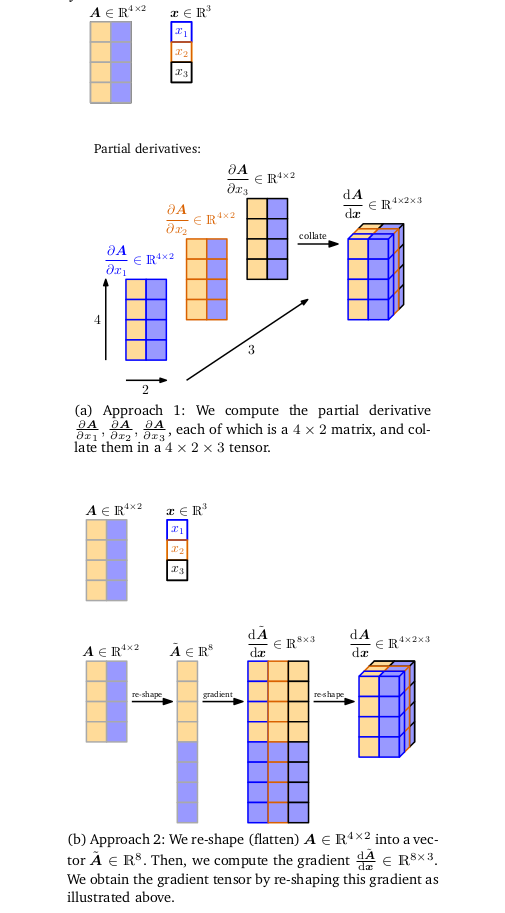
\includegraphics[width=10cm]{27}\\
\end{center}
\end{figure}
\clearpage

\subsection{Gradients of Matrices---Examples}
\textbf{Example 1---Vector and Matrix}\\
Given
\begin{equation*}
\bm{f}=\bm{Ax},\quad\bm{f}\in\mathbb{R}^{M},\quad\bm{A}\in\mathbb{R}^{M\times N},\quad\bm{x}\in\mathbb{R}^{N}
\end{equation*}
should we want to find $d\bm{f}/d\bm{A}$ the dimension of our gradient would be
\begin{equation*}
\frac{d\bm{f}}{d\bm{A}}\in\mathbb{R}^{M\times(M\times N)}
\end{equation*}
By definition, the gradient is a collection of partial derivatives, where
\begin{equation*}
\frac{d\bm{f}}{d\bm{A}}=\begin{bmatrix}
\frac{\partial f_1}{\partial\bm{A}}\\\vdots\\\frac{\partial f_M}{\partial\bm{A}}
\end{bmatrix},\quad\frac{\partial f_i}{\partial\bm{A}}\in\mathbb{R}^
{1\times(M\times N)}
\end{equation*}
To compute the partial derivatives (we require expressions for each function) it helps to explicitly write out
the matrix vector multiplication:
\begin{equation*}
f_i=\sum^{N}_{j=1}A_{ij}x_j,\quad i=1,\ldots,M
\end{equation*}
with that the partial derivatives are given as
\begin{equation*}
\frac{\partial f_i}{\partial A_{iq}}=x_q
\end{equation*}
written with respect to a row:
\begin{align*}
\frac{\partial f_i}{\partial A_{i,:}}=\bm{x}^T\in\mathbb{R}^
{1\times1\times N}\\
\frac{\partial f_i}{\partial A_{k\neq i,:}}=
\bm{0}^T\in\mathbb{R}^{1\times1\times N}
\end{align*}
where we obtain a $1\times1\times N$ sized tensor as the partial derivative of $f_i$ with respect to a row of $\bm{A}$.
Stacking the partial derivatives of the rows we get the desired
gradient
\begin{equation*}
\frac{\partial f_i}{\partial\bm{A}}=\begin{bmatrix}
\bm{0}^T\\\vdots\\\bm{0}^T\\\bm{x}^T\\\bm{0}^T\\\vdots\\\bm{0}^T
\end{bmatrix}\in\mathbb{R}^{1\times(M\times N)}
\end{equation*}
(next page)
\newpage
\noindent\textbf{Example 2---Matrix and Matrix}\\
Considering a matrix $\bm{R}\in\mathbb{R}^{M\times N}$ and
$\bm{f}:\mathbb{R}^{M\times N}\to\mathbb{R}^{N\times N}$ with
\begin{equation*}
\bm{f}(\bm{R})=\bm{R}^T\bm{R}=:\bm{K}\in\mathbb{R}^{N\times N}
\end{equation*}
where we seek the gradient $d\bm{K}/d\bm{R}$.\\
\vspace{1mm}\\
The gradient has dimensionality
\begin{equation*}
\frac{d\bm{K}}{d\bm{R}}\in\mathbb{R}^{(N\times N)\times(M\times N)}
\end{equation*}
which is a tensor, where
\begin{equation*}
\frac{dK_{pq}}{d\bm{R}}\in\mathbb{R}^{1\times(M\times N)}
\end{equation*}
for $p,q=1,\ldots,N$; where $K_{pq}$ is the $(p,q)$th entry of $\bm{K}=\bm{f}(\bm{R})$, denoting the $i$th column of $\bm{R}$
by $\bm{r}_i$, every entry of $\bm{K}$ is given by the dot product of two columns of $\bm{R}$:
\begin{equation*}
K_{pq}=\bm{r}^T_p\bm{r}_q=\sum^M_{m=1}R_{mp}R_{mq}
\end{equation*}
now we compute the partial derivative $\frac{\partial K_{pq}}{\partial R_{ij}}$ and obtain
\begin{equation*}
\frac{\partial K_{pq}}{\partial R_{ij}}=\sum^M_{m=1}
\frac{\partial}{\partial R_{ij}}R_{mp}R_{mq}=\partial_{pqij}
\end{equation*}
where
\begin{align*}
\partial_{pqij}=\begin{cases}
R_{iq}&\text{if }j=p,p\neq q\\
R_{ip}&\text{if }j=q,p\neq q\\
2R_{iq}&\text{if }j=p,p=q\\
0&\text{otherwise}
\end{cases}
\end{align*}
the desired gradient has the dimension $(N\times N)\times(M\times N)$, and every single entry of this tensor is given
by $\partial_{pqij}$, where $p,q,j=1,\ldots,N$ and $i=1,\ldots,M$.
\newpage

\subsection{Backpropagation}
\textbf{Motivation}\\
Given a function
\begin{equation*}
f(x)=\sqrt{x^2+\text{exp}(x^2)}+\cos(x^2+\text{exp}(x^2))
\end{equation*}
By application of the chain rule, and noting that differentiation is linear, we can compute the gradient as
\begin{equation*}
\frac{df}{dx}=2x\left(\frac{1}{2\sqrt{x^2+\text{exp}(x^2)}}-\sin(x^2+\text{exp}(x^2))\right)(1+\text{exp}(x^2))
\end{equation*}
Writing out the gradient in this explicit way is often impractical, and could be computationally expensive. 
When training neural network models, the \textit{backpropagation algorithm} is an effivient way to compute
the gradient of an error function with respect to parameters we want to optimise over.\\
\vspace{1mm}\\
\textbf{Backpropagation}\\
In deep learning, a function value $\bm{y}$ is computed as a many-level function composition:
\begin{equation*}
\bm{y}=(f_K\circ f_{K-1}\circ\cdots\circ f_1)(\bm{x})
=f_K(f_{K-1}(\cdots(f_1(\bm{x}))\cdots))
\end{equation*}
where $\bm{x}$ are the inputs and $\bm{y}$ are the observations, with every function $f_i$ possessing its own parameters.\\
\vspace{1mm}\\
The sequential application of such functions are organised into multiple layers:
\begin{figure}[h]
\begin{center}
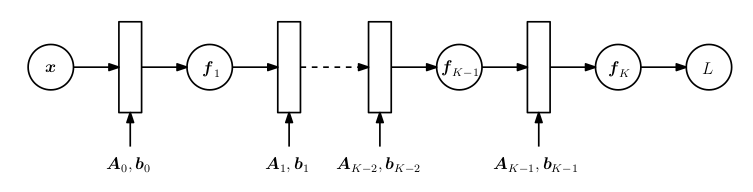
\includegraphics[width=10cm]{28}\\
\end{center}
we have functions $f_i(x_{i-1})=\sigma(\bm{A}_{i-1}\bm{x}_{i-1}+\bm{b}_{i-1})$ in the $i$th layer, where 
$\bm{x}_{i-1}$ is the output of the layer $i-1$ and $\sigma$ an activation function like the logistic sigmoid $\frac{
1}{1+e^{-x}}$. To train these models we require a gradient of the loss function with respect to all model parameters
$\bm{A}_j,\bm{b}_j$ where $j=1,\ldots,K$; thus we need to compute the gradients with respect to each layer.
\end{figure}\\
(next page)
\newpage
\noindent(cont.) Say we have inputs $\bm{x}$ and observations $\bm{y}$ and a network structure defined by
\begin{align*}
\bm{f}_0&:=\bm{x}\\
\bm{f}_i&:=\sigma_i(\bm{A}_{i-1}\bm{f}_{i-1}+\bm{b}_{i-1}),\quad
i=1,\ldots,K
\end{align*}
we may be interested in finding $\bm{A}_j,\bm{b}_j$ for $j=0,\ldots,K-1$ such that the squared loss
\begin{equation*}
L(\bm{\theta})=||\bm{y}-\bm{f}_K(\bm{\theta},\bm{x})||^2
\end{equation*}
is minimised, where $\bm{\theta}=\{\bm{A}_0,\bm{b}_0,\ldots,
\bm{A}_{K-1},\bm{b}_{K-1}\}$.\\
\vspace{1mm}\\
To obtain the gradients with respect to the parameter set $\bm{\theta}$, we require the partial derivatives of L with
respect to the parameters $\bm{\theta}_j=\{\bm{A}_j,\bm{b}_j\}$
of each layer $j=0,\ldots,K-1$. The chain rule allows us to determine the partial derivatives as
\begin{align*}
\frac{\partial L}{\partial\bm{\theta}_{K-1}}&=
\frac{\partial L}{\partial\bm{f}_K}\frac{\partial\bm{f}_K}{\partial\bm{\theta}_{K-1}}\\
\frac{\partial L}{\partial\bm{\theta}_{K-2}}&=
\frac{\partial L}{\partial\bm{f}_K}\frac{\partial\bm{f}_K}{\partial\bm{f}_{K-1}}
\frac{\partial\bm{f}_{K-1}}{\partial\bm{\theta}_{K-2}}\\
\frac{\partial L}{\partial\bm{\theta}_{K-3}}&=
\frac{\partial L}{\partial\bm{f}_K}\frac{\partial\bm{f}_K}{\partial\bm{f}_{K-1}}
\frac{\partial\bm{f}_{K-1}}{\partial\bm{f}_{K-2}}
\frac{\partial\bm{f}_{K-2}}{\partial\bm{\theta}_{K-3}}\\
\frac{\partial L}{\partial\bm{\theta}_i}&=
\frac{\partial L}{\partial\bm{f}_K}
\frac{\partial\bm{f}_K}{\partial\bm{f}_{K-1}}\cdots
\frac{\partial\bm{f}_{i+2}}{\partial\bm{f}_{i+1}}
\frac{\partial\bm{f}_{i+1}}{\partial\bm{\theta}_{i}}
\end{align*}
see that, assuming one has already computed the partial derivatives $\partial L/\partial\bm{\theta_}{i+1}$, then most 
of the computation can be reused to compute $\partial L/\partial\bm{\theta_}{i}$.
\newpage

\subsection{Automatic Differentiation}
Backpropagation is really a special case of a general technique of numerical analysis called 
\textit{automatic differentiaton}. We can think of automatic
differentiation as a set of techniques to numerically evaluate the gradient of a function by working with intermediate
variables and applying the chain rule.\\
\vspace{1mm}\\
Consider data flow from inputs $x$ to $y$ via some intermediate variables $a,b$; if we were to compute the derivative $dy/dx$,
we would apply the chain rule and obtain
\begin{equation*}
\frac{dy}{dx}=\frac{dy}{db}\frac{db}{da}\frac{da}{dx}
\end{equation*}
Also see that due to the associativity of matrix multiplication, we can choose between \textit{forward mode} and
\textit{reverse mode}:
\begin{align*}
\frac{dy}{dx}=\left(\frac{dy}{db}\frac{db}{da}\right)\frac{da}{dx}\\
\frac{dy}{dx}=\frac{dy}{db}\left(\frac{db}{da}\frac{da}{dx}\right)
\end{align*}
Where the first equation would be reverse mode since the gradients are propagated backward through the graph; while the 
second being forward mode.\\
\vspace{1mm}\\
\textbf{Formalisation}\\
Let $x_1,\ldots,x_d$ be the input variables to a function, 
$x_{d+1},\ldots,x_{D-1}$ be the intermediate variables, and 
$x_D$ the output variable; then the computation graph can be 
expressed as follows
\begin{equation*}
\text{For }i=d+1,\ldots,D:\quad x_i=g_i(x_{\text{Pa}(x_i)})
\end{equation*}
where the $g_i(\cdot)$ are elementary functions and $x_{\text{Pa}(x_i)}$ are the parent nodes of the variable $x_i$ in 
the computation graph. Given a function defined this way
we can use the chain rule to compute the derivative of the function in a step-by-step fashion.
We have $f=x_D$ (as defined since $f$ is the output); for all other variables we apply the chain rule:
\begin{equation*}
\frac{\partial f}{\partial x_i}=\sum_{x_j:x_i\in\text{Pa}(x_j)}
\frac{\partial f}{\partial x_j}\frac{\partial x_j}{\partial x_i}=
\sum_{x_j:x_i\in\text{Pa}(x_j)}
\frac{\partial f}{\partial x_j}\frac{\partial g_j}{\partial x_i}
\end{equation*}
The automatic differentiation approach works whenever we have a function that can be expressed as a computation graph
with differentiable elementary functions.\\
(next page)
\newpage
\noindent\textbf{Example}\\
Automatic differentiation is essentially the formalisation of the following instructive example. Here we use reverse mode 
automatic differentiation (which in the context of neural networks is computationally significantly cheaper 
due to the tendency for high input dimensionality): Consider the function
\begin{equation*}
f(x)=\sqrt{x^2+\text{exp}(x^2)}+\cos(x^2+\text{exp}(x^2))
\end{equation*}
see that if we were to implement a function $f$ on a computer, we would be able to save some computation by using 
\textit{intermediate variables}:
\begin{align*}
a=x^2,\quad&\quad
b=\text{exp}(a)\\
c=a+b,\quad&\quad
d=\sqrt{c}\\
e=\cos(c),\quad&\quad
f=d+e
\end{align*}
Notice how the last variable is `connected' to the first variable by a sequence of intermediate variables (this is the same 
kind of thinking that occurs when applying the chain rule). 
Also note that the preceding set of equations requires fewer operations than a direct implementation of the function 
as fully defined in the beginning; the corresponding \textit{computation graph} shows the flow of data and 
computations required to obtain the final function output:
\begin{figure}[h]
\begin{center}
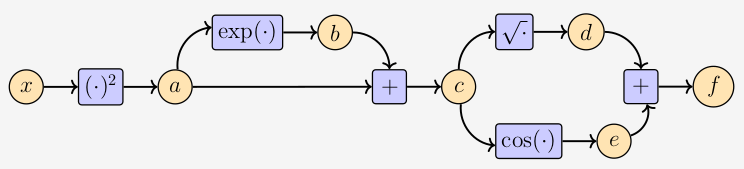
\includegraphics[width=10cm]{29}\\
\end{center}
computation graphs are representations that are widely used in implementation of neural network software libraries.
We can directly compute the derivatives of the intermediate variables with respect to their corresponding inputs 
(which is easy since they are elementary functions):
\begin{align*}
\frac{\partial a}{\partial x}=2x,\quad&\quad
\frac{\partial b}{\partial a}=\text{exp}(a)\\
\frac{\partial c}{\partial a}=1=\frac{\partial c}{\partial b},
\quad&\quad\frac{\partial d}{\partial c}=\frac{1}{2\sqrt{c}}\\
\frac{\partial e}{\partial c}=-\sin(c),\quad&\quad
\frac{\partial f}{\partial d}=1=\frac{\partial f}{\partial e}
\end{align*}
(next page)
\end{figure}
\newpage
\noindent and by looking at the computation graph we can compute $\partial f/\partial x$ by working backward from the output
to obtain
\begin{align*}
\frac{\partial f}{\partial c}&=\frac{\partial f}{\partial d}
\frac{\partial d}{\partial c}
+\frac{\partial f}{\partial e}\frac{\partial e}{\partial c}\\
\frac{\partial f}{\partial b}&=\frac{\partial f}{\partial c}
\frac{\partial c}{\partial b}\\
\frac{\partial f}{\partial a}&=\frac{\partial f}{\partial b}
\frac{\partial b}{\partial a}+\frac{\partial f}{\partial c}
\frac{\partial c}{\partial a}\\
\frac{\partial f}{\partial x}&=\frac{\partial f}{\partial a}
\frac{\partial a}{\partial x}
\end{align*}
where we think of each of the derivatives as a variable.
\newpage

\subsection{}




















\end{document}
